\documentclass[a4paper, 12pt, titlepage,oneside,drop]{kthesis}
\usepackage{a4wide}            
\usepackage[T1]{fontenc}
\usepackage{lmodern}
\usepackage[utf8]{inputenc}    
\usepackage[swedish,english]{babel}
\usepackage{cite}
\usepackage[pdftex]{rotating,graphicx}
\usepackage{epstopdf}
\usepackage{graphicx}   % For eps figures
\usepackage{csvsimple}
\usepackage{amsmath}
\usepackage{multirow}
\usepackage{rotating}
\usepackage{amsmath}
\usepackage{amsfonts}
\usepackage{amssymb}
\usepackage{amsbsy}
\pagestyle{headings}
\usepackage[table]{xcolor}% http://ctan.org/pkg/xcolor
\usepackage{color}
\usepackage{graphicx}
\usepackage{epsfig}
\usepackage{float}
\newtheorem{thm}{Theorem}
\usepackage{tikz}
\usetikzlibrary{shapes,arrows}
\usepackage[hang,indention=-0.5cm,width=14cm,font=small,labelfont=bf,labelsep=period]{caption}
\usepackage{palatino}
\usepackage{fixltx2e}
\usepackage{siunitx}
\usepackage{booktabs}
\usepackage{caption}
\usepackage{url}
\usepackage{pdfpages}
\usepackage{afterpage}
%\usepackage[width=1.2\textwidth]{caption}
\newcommand\blankpage{%
    \null
    \thispagestyle{empty}%
    \addtocounter{page}{-1}%
    \newpage}


\renewcommand{\thechapter}{\Roman{chapter}} 
 
\setlength{\parskip}{6pt}  % 12 pt = hopp mellan stycken
\setlength{\parindent}{0pt} % 0 pt  = indrag
\makeatletter
\newcommand{\rmnum}[1]{\romannumeral #1}
\newcommand{\Rmnum}[1]{\expandafter\@slowromancap\romannumeral #1@}
\makeatother

\usepackage{titlesec}
\titleformat{\chapter}[hang] 
{\normalfont\LARGE\bfseries}{\chaptertitlename\ \thechapter}{1em}{}


%And here the document begins!

\begin{document}




\bibliographystyle{ieeetr}

\def\hath{{H}}
\def\wf {\Psi(\{ {\textbf r}_{i}, {\textbf R}_{I} \})}
\def\wfbo{\Psi_{{BO}}({{\textbf r}_{{i}}},{\textbf R} )}
\def\wfh{\Psi^{{H}}(\{ {\textbf r}_{{i}}\})}
\def\wfks{\Psi^{{KS}}(\{ {\textbf r}_{{i}}\})}
\def\wfhit<#1>{\Psi_{{H}}^{#1}({{\textbf r}_{{i}}})}
\def\bwf<#1><#2>{\Psi_{#1}^{KS}({\textbf r}_{#2})}
\def\bwff<#1><#2>{\phi_{#1}({\textbf r}_{#2})}
\def\bwfn<#1><#2>{\phi_{#1}({\textbf r}{#2})}
\def\bwfnn<#1><#2>{\phi_{#1}({\textbf r}_{#2})}
\def\wfbloch<#1><#2>{\Psi_{#1,#2}({\textbf r})}
\def\ubloch<#1><#2>{u_{#1,#2}({\textbf r})}
\def\ebloch<#1><#2>{E_{#1,#2}}
\def\bwfc<#1><#2><#3>{\phi_{#1}^{#3}({\textbf r}_{#2})}
\def\sumi<#1> {\sum\limits_{ #1}}
\def\sumij<#1><#2> {\sum\limits_{ #1,#2}}
\def\suminj<#1><#2> {\sum\limits_{{#1} \neq {#2}}}
\def\coefkhe{-\frac{\hbar^2}{2 m_{e}}}
\def\coefkhn{-\frac{\hbar^2}{2 M_{I}}}
\def\nablaia<#1> {{\nabla}_{{#1}}^{2}}
\def\moperater{-i\hbar \nabla}
\def\sumg<#1>{{\sum\limits_{{#1}}}}    
\def\sumlm<#1><#2>{\sum\limits_{{#1}{#2}}}
\def\coeff<#1><#2><#3>{C_{#1,{\textbf k_0} +\textbf{#2}}^{#3}}      %C_{j,k_0+G}^{*}
\def\expkg<#1><#2>{e^{i(\textbf{#1}+\textbf{#2})\textbf{r}}}          %exp{i(k+G)r}
\def\expg<#1>{e^{i{\textbf #1} {\textbf r}}}                         %exp{iGr}
%\def\bwf<#1>{\phi_{\textbf{k_0}+\textbf{#1}}^{\textbf{APW}}(\textbf{r})}          %phi_{k_0+G}  
\def\chig<#1>{{\chi_{\textbf kk_0}(\textbf{#1})}}                  %chi_{kk_0}{G}
%\def\hath{ | \hat{H} | }           
\def\kplusg<#1><#2>{(\textbf{#1}+\textbf{#2})}                    % k+G 
\def\radiaf<#1><#2>{f_{{\ell}^{\prime}{m}^{\prime}} (r_{\alpha},\textbf{#1+#2})}    % f(r,k+G)
\def\radiafc<#1><#2><#3>{f_{{\ell}^{\prime}{m}^{\prime}}^{#3} (r_{\alpha},\textbf{#1+#2})}    % f(r,k+G)
\def\bradiaf{u^{\alpha}_{q,\ell^{\prime}}(r_{\alpha},E_{\ell^{\prime}})}              %u(r_\alpha) did not contain the Energy
\def\sphfr<#1><#2><#3> {{Y_{#1}^{#3}(\hat{\textbf{#2}}_{\alpha})}}                             %Y_{lm}(\hat{r})
\def\sphfq<#1><#2><#3> {{Y_{#1}^{#3}(\widehat{{\textbf{#2}}})}}                             %Y_{lm}(\hat{q})
\def\gaucoe{C_{{\ell{m}},{\ell^{\prime}m^{\prime}},{\ell^{\prime\prime}m^{\prime\prime}}}}  %Gaunt coefficient
\def\potvgir{V_{\textbf G^{\prime\prime} }}                                %V{G}
\def\potvmt{V^{\alpha}_{{\ell}^{\prime\prime}{m}^{\prime\prime}} (r_{\alpha})}  %V{lm,r}     
\def\fracatom<#1> {e^{i \textbf{#1} \textbf R^\alpha }}   % exp(iq\def\nablai2<#1> {{\nabla}_{\textit{#1}}^{2}}R)
\def\bessf<#1>{j_{\ell}({#1}r_{\alpha})}     %j_l(kr)
\def\dr{\mathrm{d}\textbf{r}}
\def\chikp<#1><#2>{{\chi_{#1,#2}(\textbf{r})}}  
\newcommand{\se}{Schrödinger equation}
\def\hm{Hamiltonian }
\def\cigs{\mathrm  { CuIn_{1-\textit{x}}Ga_\textit{x}Se_2}}
\def\czts{\mathrm {Cu_2ZnSnS_2} } 
\def\cztse{\mathrm { Cu_2ZnSnSe_2}}
\def\cztsse{\mathrm  { CuZnSn(S_{1-\textit{x}}Se_{\textit{x}})_4}}


\pagenumbering{roman}
\setcounter{page}{1}

\begin{center}




 
\epsfig{file=kth_svv_indu_eng_manage.eps,width=4 cm}
  \vspace{5 cm}





  \vspace{12pt}
  \textsc{\LARGE{\textbf{Exploring the electronic and optical properties of Cu(In,Ga)Se\textsubscript{2} }}}
  \vspace{12pt}

  \vspace{5 cm}

  \textsc{\large{Rongzhen Chen}}


  \vfill 

  \ 

  \large{Licentiate Thesis}
  \\
  \large{School of Industrial Engineering and Management,
  Department of Materials Science and Engineering,
  KTH, Sweden, 2015}

\end{center}

 \thispagestyle{empty}



\newpage
\setcounter{page}{2}
\thispagestyle{empty}
\
\vfill

\begin{flushright}
 Materialvetenskap\\
 KTH\\
\hfill SE-100 44 Stockholm\\ ISBN 978-91-7501-323-8  \hfill
Sweden\\
\end{flushright}


\vspace{5mm}

Akademisk avhandling som med tillstånd av Kungliga Tekniska
Högskolan framlägges till offentlig granskning för avläggande av
licentiatexamen fredagen den 13rd March 2015 kl 10:00 i konferensrummet, Materialvetenskap, Kungliga Tekniska
Högskolan,\linebreak Brinellvägen 23, Stockholm.

\vspace{5mm}

\copyright \hspace{3pt} {Rongzhen Chen, March, 2015}

\vspace{5mm}

Tryck: Universitetsservice US AB

\newpage


\begin{abstract}
 \addcontentsline{toc}{chapter}{Abstract}
\begin{comment}
In order to reduce the high dependence on fossil fuels and oil, solar energy is one of the alternatives. Thin film photovoltaic (PV) technology is one of the solar energy,  and there are several rather important absorber materials in the PV technology, such as the cadmium
telluride (CdTe) and chalcopyrite copper indium gallium diselenide (CIGS). The maximum conversion efficiency of CIGS had reached 23.3\% in the National Renewable Energy Laboratory, Golden, Colorado, U.S.A. Therefore,
the accurate information for this kind of absorber materials is of great importance in order to design the photovoltaic materials. 

In the licentiate thesis, two researches are investigated for CIGS. (1) Parameterization of the band dispersion for the uppermost three valence bands (VBs) and the lowest conduction
band (CB) for CuInSe\textsubscript{2}, CuIn\textsubscript{0.5}Ga\textsubscript{0.5}Se\textsubscript{2}, and CuGaSe\textsubscript{2} is modeled, which is based on the $\textbf{k} \cdot \textbf{p}$ method, but extended it up to high order.
It demonstrates that the VBs and CB are quite non-parabolic away from the $\Gamma$ point, which implies that the effective mass on $\Gamma$ point is not suitable to describe the materials properties such as 
band filling and strong excitation effects. (2) The dielectric function spectra of CuIn\textsubscript{0.5}Ga\textsubscript{0.5}Se\textsubscript2 is calculated. It is compared with the
experiment result based on CuIn\textsubscript{0.7}Ga\textsubscript{0.3}Se\textsubscript{2} at 40 K and 300 K, which demonstrates that the overall shape of dielectric function spectra is in good agreement for both of calculation and 
experiment.

\noindent Three uppermost VBs and the lowest CB of CIGS are parameterized in order to better understand and describe the anisotropy and non-parabolic of the energy dispersion.
In order to illustrate the non-parabolic of the band dispersion, the effective electron and hole mass tensors are obtained in four symmetry directions. To further illustrate
the non-parabolic, the constant energy surface are calculated for the three topmost VBs as well as the lowest CB. The density-of-states (DOS), Fermi energy and the carrier
concentrations are calculated and analyzed based on this parameterization as well. The results are compared with the parabolic band energy approximation. 


\noindent The dielectric function spectra of CuIn\textsubscript{0.5}Ga\textsubscript{0.5}Se\textsubscript{2} is determined by the all electron and full-potential linearized augmented plane wave calculations (FPLAPW). 
It shows a good agreement with the result from spectroscopic ellipsometry, which illustrates the results of CuIn\textsubscript{0.7}Ga\textsubscript{0.3}Se\textsubscript{2} at 40 K and 300 K. Furthermore, 
the probable electronic origins of observed interband critical points are discussed. The band to band analysis
of the contribution to the total imaginary part of dielectric function spectrum is explored as well.
\end{comment}

\noindent Chalcopyrite copper indium gallium diselenide (CuIn\textsubscript{1-x}Ga\textsubscript{x}Se\textsubscript{2})
is today a commercially important material in the thin-film solar cell technology, and it is also in many aspects a very interesting material from a scientifically point of view.

\noindent In this licentiate thesis, details in the electronic structure of CuIn\textsubscript{1-x}Ga\textsubscript{x}Se\textsubscript{2} alloy ($x$ = 0.0, 0.5, and 1.0) and its optical response are explored by means of the all-electron and full-potential linearized augmented plane wave method in conjunction with the density functional theory. 
The energy band dispersions are parameterized for the three uppermost valence bands (VBs;  $v$1 to $v$3) and the lowest conduction band (CB; $c$1), based on the $\mathbf k \cdot \mathbf p$ method but expanded up to high order. 
To illustrate the non-parabolic, the constant energy surfaces are presented for the three topmost VBs as well as for the lowest CB. 

It is demonstrated that the VBs and CB are anisotropic at the $\Gamma$-point, and even more anisotropic and non-parabolic away from the $\Gamma$-point. The effect originates from the crystal-field and the spin-orbit split-off energies. This implies that the $\Gamma$-point effective mass is not suitable to describe the materials properties such as band filling and strong excitation effects. 
Instead, the thesis provides the effective electron and hole mass tensors at the $\Gamma$-point in the Brillouin zone, 
but also an energy-dependent effective mass which can better describe both the transport and band filling effect
in further experimental and theoretical analyses of the materials.  

Based on the parametrized energy bands, the density-of-states as well as temperature dependence of the Fermi energy and carrier concentrations are determined for intrinsic and $p$-type CuIn\textsubscript{1-x}Ga\textsubscript{x}Se.
The results are compared with corresponding results for the commonly used parabolic approximation of the bands. 



Furthermore, the dielectric function of CuIn\textsubscript{0.5}Ga\textsubscript{0.5}Se\textsubscript{2} 
is calculated, and the band-to-band optical transitions are analyzed. The electronic origins of the observed interband critical points of the  optical response are discussed. 
The theoretical results are compared with the experiment data based on CuIn\textsubscript{0.7}Ga\textsubscript{0.3}Se\textsubscript{2} at the temperatures 40 and 300 K, demonstrating that the overall shapes of the calculated and measured dielectric function spectra are in good agreement. 
We find that $v$1$-c$1 and $v$2$-c$1 transitions in the Brillouin zone edge are responsible for the main absorption peaks
at 3.00 and 3.09 eV, where $v$1 and $v$2 represent the first uppermost valence band and the second uppermost valence band, respectively. However, also the energetically lower VBs contribute to the high absorption coefficient. 

\newpage
\end{abstract}


\blankpage


\setcounter{page}{5}

\section*{Preface} \addcontentsline{toc}{chapter}{Preface}

\subsection*{List of included publications:}

\begin{enumerate}
\renewcommand{\labelenumi}{\Roman{enumi}}
%\item{} \textbf{Parameterization of $CuIn_{1−x}Ga_{x}Se_2$ (x = 0, 0.5, and 1) energy bands}
\item{}  \textbf{Parameterization of $\mathbf {CuIn_{1-x}Ga_{x}Se_2}$ (x = 0, 0.5, and 1) energy bands}
\\\textbf{R. Chen} and C. Persson, \textit{Thin Solid Films} {\textbf {519}}, 7503 (2011).



\item{}\textbf{Band-edge density-of-states and carrier concentrations in intrinsic and $p$-type $\mathbf {CuIn_{1-x}Ga_{x}Se_2}$}
\\\textbf{R. Chen} and C. Persson, \textit{J. Appl. Phys.} {\textbf {112}}, 103708 (2012).

\item{} \textbf{Dielectric function spectra at 40 K and critical-point energies for $\mathbf {CuIn_{0.7}Ga_{0.3}Se_2}$}
\\ S.G. Choi, \textbf{R. Chen}, C. Persson, T.J. Kim, S.Y. Hwang, Y. D. Kim, and L. M. Mansfield,
\textit{Appl. Phys. Lett. } {\textbf {101}}, 261903 (2012).

\end{enumerate}
\subsection*{My contribution to the publications:}

\textbf{Paper I:} modeling, analysis of result, literature survey;
the manuscript was written jointly.\\
\textbf{Paper II:} modeling, analysis of result, literature survey; main part of the manuscript was written.\\
\textbf{Paper \Rmnum{3}:} all calculations, analysis of the theoretical part, part of literature survey;
the manuscript was written jointly.\\

\subsection*{Publications not included in the thesis:}
\begin{enumerate}
\renewcommand{\labelenumi}{\Roman{enumi}}
\setcounter{enumi}{3}

\subsubsection*{Book chapter:}
\item{}\textbf{Electronic structure and optical properties from first-principles modeling} \\
C. Persson, \textbf{R. Chen}, H. Zhao, M. Kumar, and D. Huang, Chapter in “Copper zinc tin sulphide-based thin film solar cells”,
edited by K. Ito ({\textit John Wiley $\&$ Sons}, 2014).


%\end{enumerate}

\subsubsection*{International conference contributions:}
%\begin{enumerate}
\renewcommand{\labelenumi}{\Roman{enumi}}
\setcounter{enumi}{4}

\item{} \textbf{Band structure and optical properties of CuInSe\textsubscript{2}}
\\ \textbf{R. Chen} and C. Persson, 
\textit{Advanced Materials Research Journal} {\textbf 894}, 254 (2014). \\
\textit{4th Int. Conf. on Adv. Mater. Res (ICAMR$-$4), Macao, China, 23$-$24 Jan. 2014.}


\item{} \textbf{Electronic modeling and optical properties of CuIn\textsubscript{0.5}Ga\textsubscript{0.5}Se\textsubscript{2} thin film solar cell}
\\ \textbf{R. Chen} and C. Persson,
\textit{J. Appl. Math. \& Phys.} {\textbf 2}, 41 (2014). \\
\textit{Conf. on New Adv. Cond, Matter Phys. (NACMP 2014), Shenzhen, 14$-$16 Jan 2014.}

\end{enumerate}

\newpage
\setcounter{page}{7}
\setcounter{secnumdepth}{3}
\setcounter{tocdepth}{3}
\renewcommand\contentsname{Table of Contents}

\tableofcontents



\newpage
\pagenumbering{arabic}
\renewcommand{\thesection}{\arabic{chapter}.\arabic{section}}  
\renewcommand{\thetable}{\arabic{chapter}.\arabic{table}}  
\renewcommand{\thefigure}{\arabic{chapter}.\arabic{figure}} 
\renewcommand{\theequation}{\arabic{chapter}.\arabic{equation}} 
\renewcommand{\chaptername}{}



\chapter{INTRODUCTION}

With the increasing energy consumption, more and more energy or power is needed. According to the statistical review of world energy on 2014 \cite{bp} (\textbf{Fig. \ref{wpec}}),
the required energy is mainly satisfied by fossil fuels (mainly coal, petroleum, and natural gas), with a market share of around 87\%. The total energy consumption is between 12000 and 13000 million tonnes oil
equivalent (MTOE), which is equivalent to around 15 terawatts \cite{xie2014creating}. Normally, one light bulb at our homes consumes between 50 and 100 watts of energy, and 1 terawatt implies 10 billion of 100 watts light bulbs are lighted at the
same time. Unfortunately, fossil fuels are very limited energy and non-renewable resources. One day, which is not far from now, they will be dissipated due to the energy consumption growth.

\begin{figure}[H]
\centering
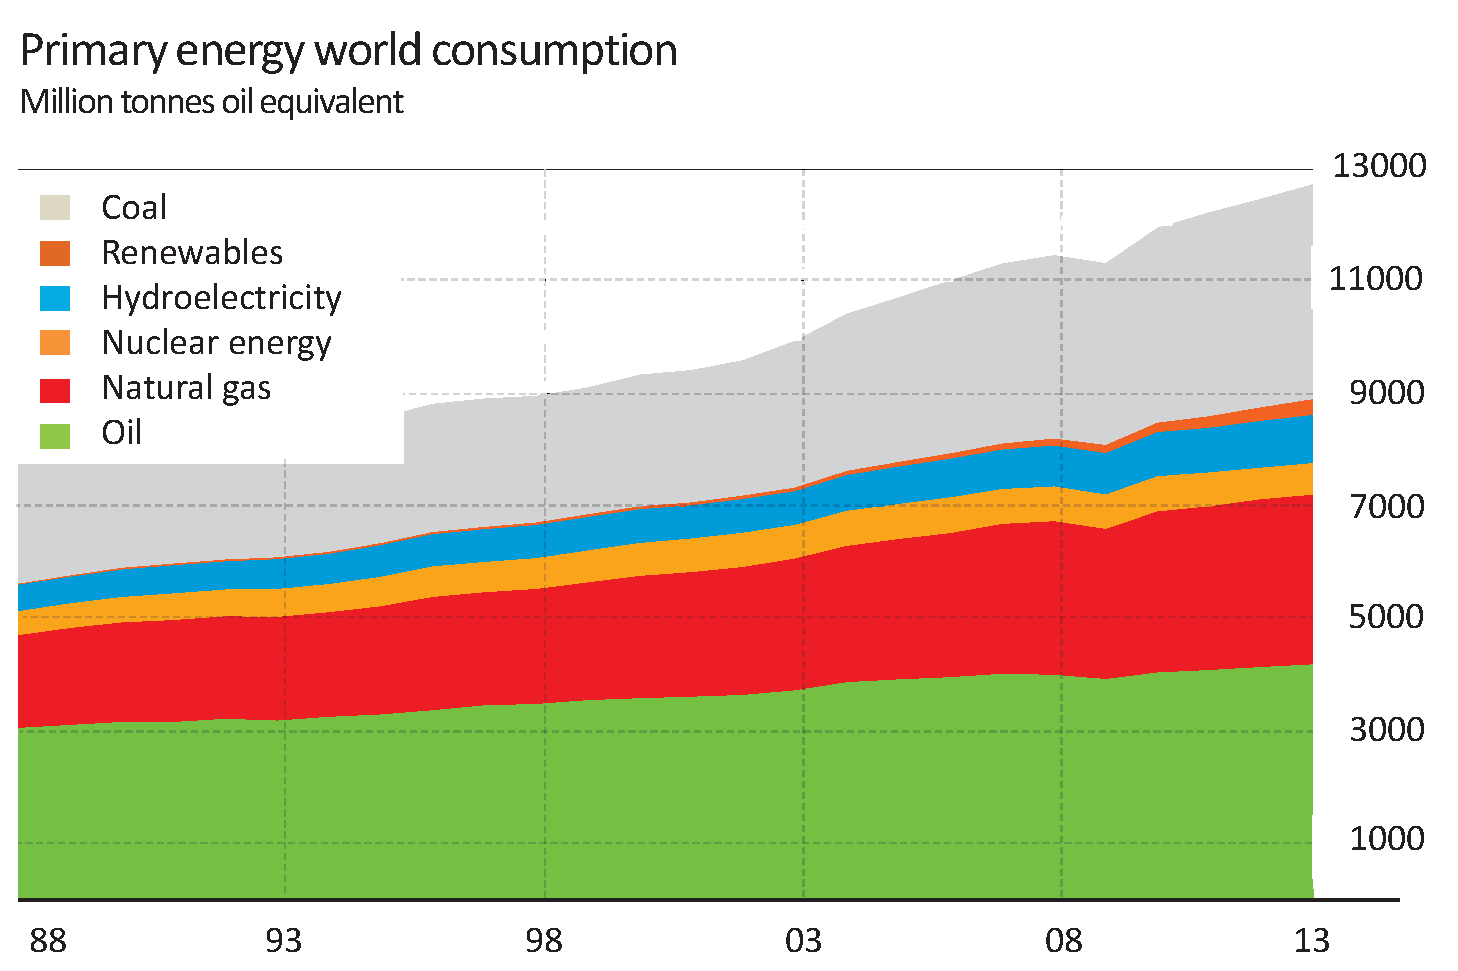
\includegraphics[scale=0.4]{energy.eps}
\caption{Primary energy world consumption in 2014 \cite{bp}.}
\label{wpec}
\end{figure}

By the year of 2050, the total world energy consumption will double \cite{iea}. Therefore, it is urgent to explore more sustainable and environmentally friendly energy sources. In \textbf{Fig. \ref{wpec}},
renewable energy (mainly solar energy, wind power, and geothermal energy) in 2013 accounts for around 2\% of the energy consumption globally. It is important to focus on renewable energy research from a 
long term point of view. Solar energy technologies are one of the hot topics among renewable energy research considering the point of CO\textsubscript{2} free, reliable energy supply, and operation in silence.

Solar energy technologies are a way to produce electricity from sunlight. Sunlight is a portion of radiation by the sun, such as ultraviolet, visible,
and infrared light. Spectrum of the sunlight is given in \textbf{Fig. \ref{spectrumsun}}. Solar spectrum is established
by air mass (AM) at the photovoltaic (PV) industry, which defines a direct optical path length through the Earth's atmosphere \cite{smestad2002optoelectronics}. AM1.5 and AM0 are two important references of spectra:
AM1.5 is the air mass at a solar zenith angle of 48.19 degree, and AM0 is the solar spectrum outside of the atmosphere. Generally, solar spectrum at AM1.5 is used in PV field in order to standardize solar cell measurements. 
In \textbf{Fig. \ref{spectrumsun}}, absorption in the atmosphere is quite strong by gases, dust, and aerosols, as well as scattering light from air molecules \cite{seinfeld2012atmospheric}.

\begin{figure}[H]
\centering
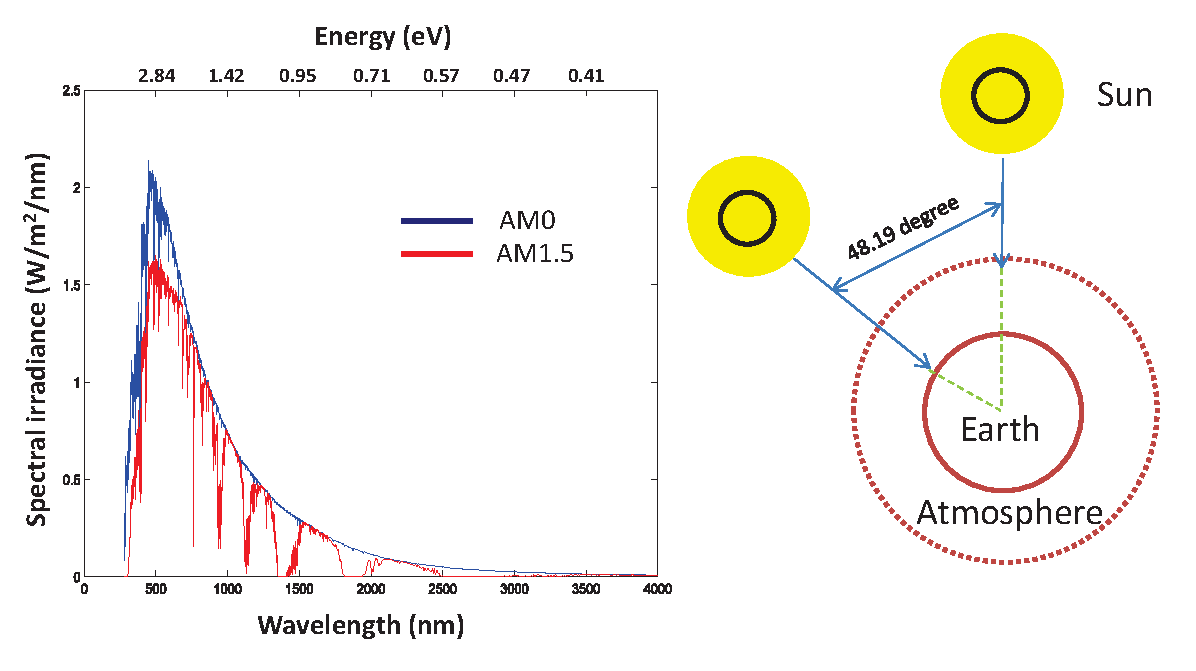
\includegraphics[scale=0.6]{spectrum.eps}
\caption{Spectral irradiance AM1.5 and AM0.}
\label{spectrumsun}
\end{figure}

There are three kinds of solar energy technologies \cite{boyle2004renewable,Chiras201007}. The first one is solar thermal technology, which utilizes flat sunlight collector plates to harness energy from sunlight to heat water
for use in industries, homes, and pools. The advantage of solar thermal technology is that the conversion efficiency is relatively higher compared with other solar energy technologies. The second one is 
solar chemical technology, which takes advantage of solar energy by absorbing sunlight in a chemical reaction. However, the conversion efficiency of this technology is quite low. The last one is solar photovoltaics (solar cell), which is a way
to utilize solar panels to convert sunlight into electricity. The installation of solar panel is easier, and it occupies less space and needs less maintenance compared with solar thermal technology.
The conversion efficiency of solar cell is higher than the one of solar chemical technology. However, all the three solar energy technologies are environmentally friendly.


\section{Solar cells}
In the worldwide, the conversion efficiencies in all different types of solar cells are improved remarkably \cite{nrel}. From \textbf{Fig. \ref{nrel}}, the highest efficiency for multijunction cells, crystalline silicon (c-Si) cells,
thin-film technologies, and new emerging cells are 44.7\%, 27.6\%, 23.3\%, and 20.1\% \cite{dimroth2014wafer, jones2009new, ward2014cu, green2015solar}. Therefore, solar cell is a very important and promising way to produce renewable energy.


\begin{sidewaysfigure}
\captionsetup{width=1\textwidth}
\centering
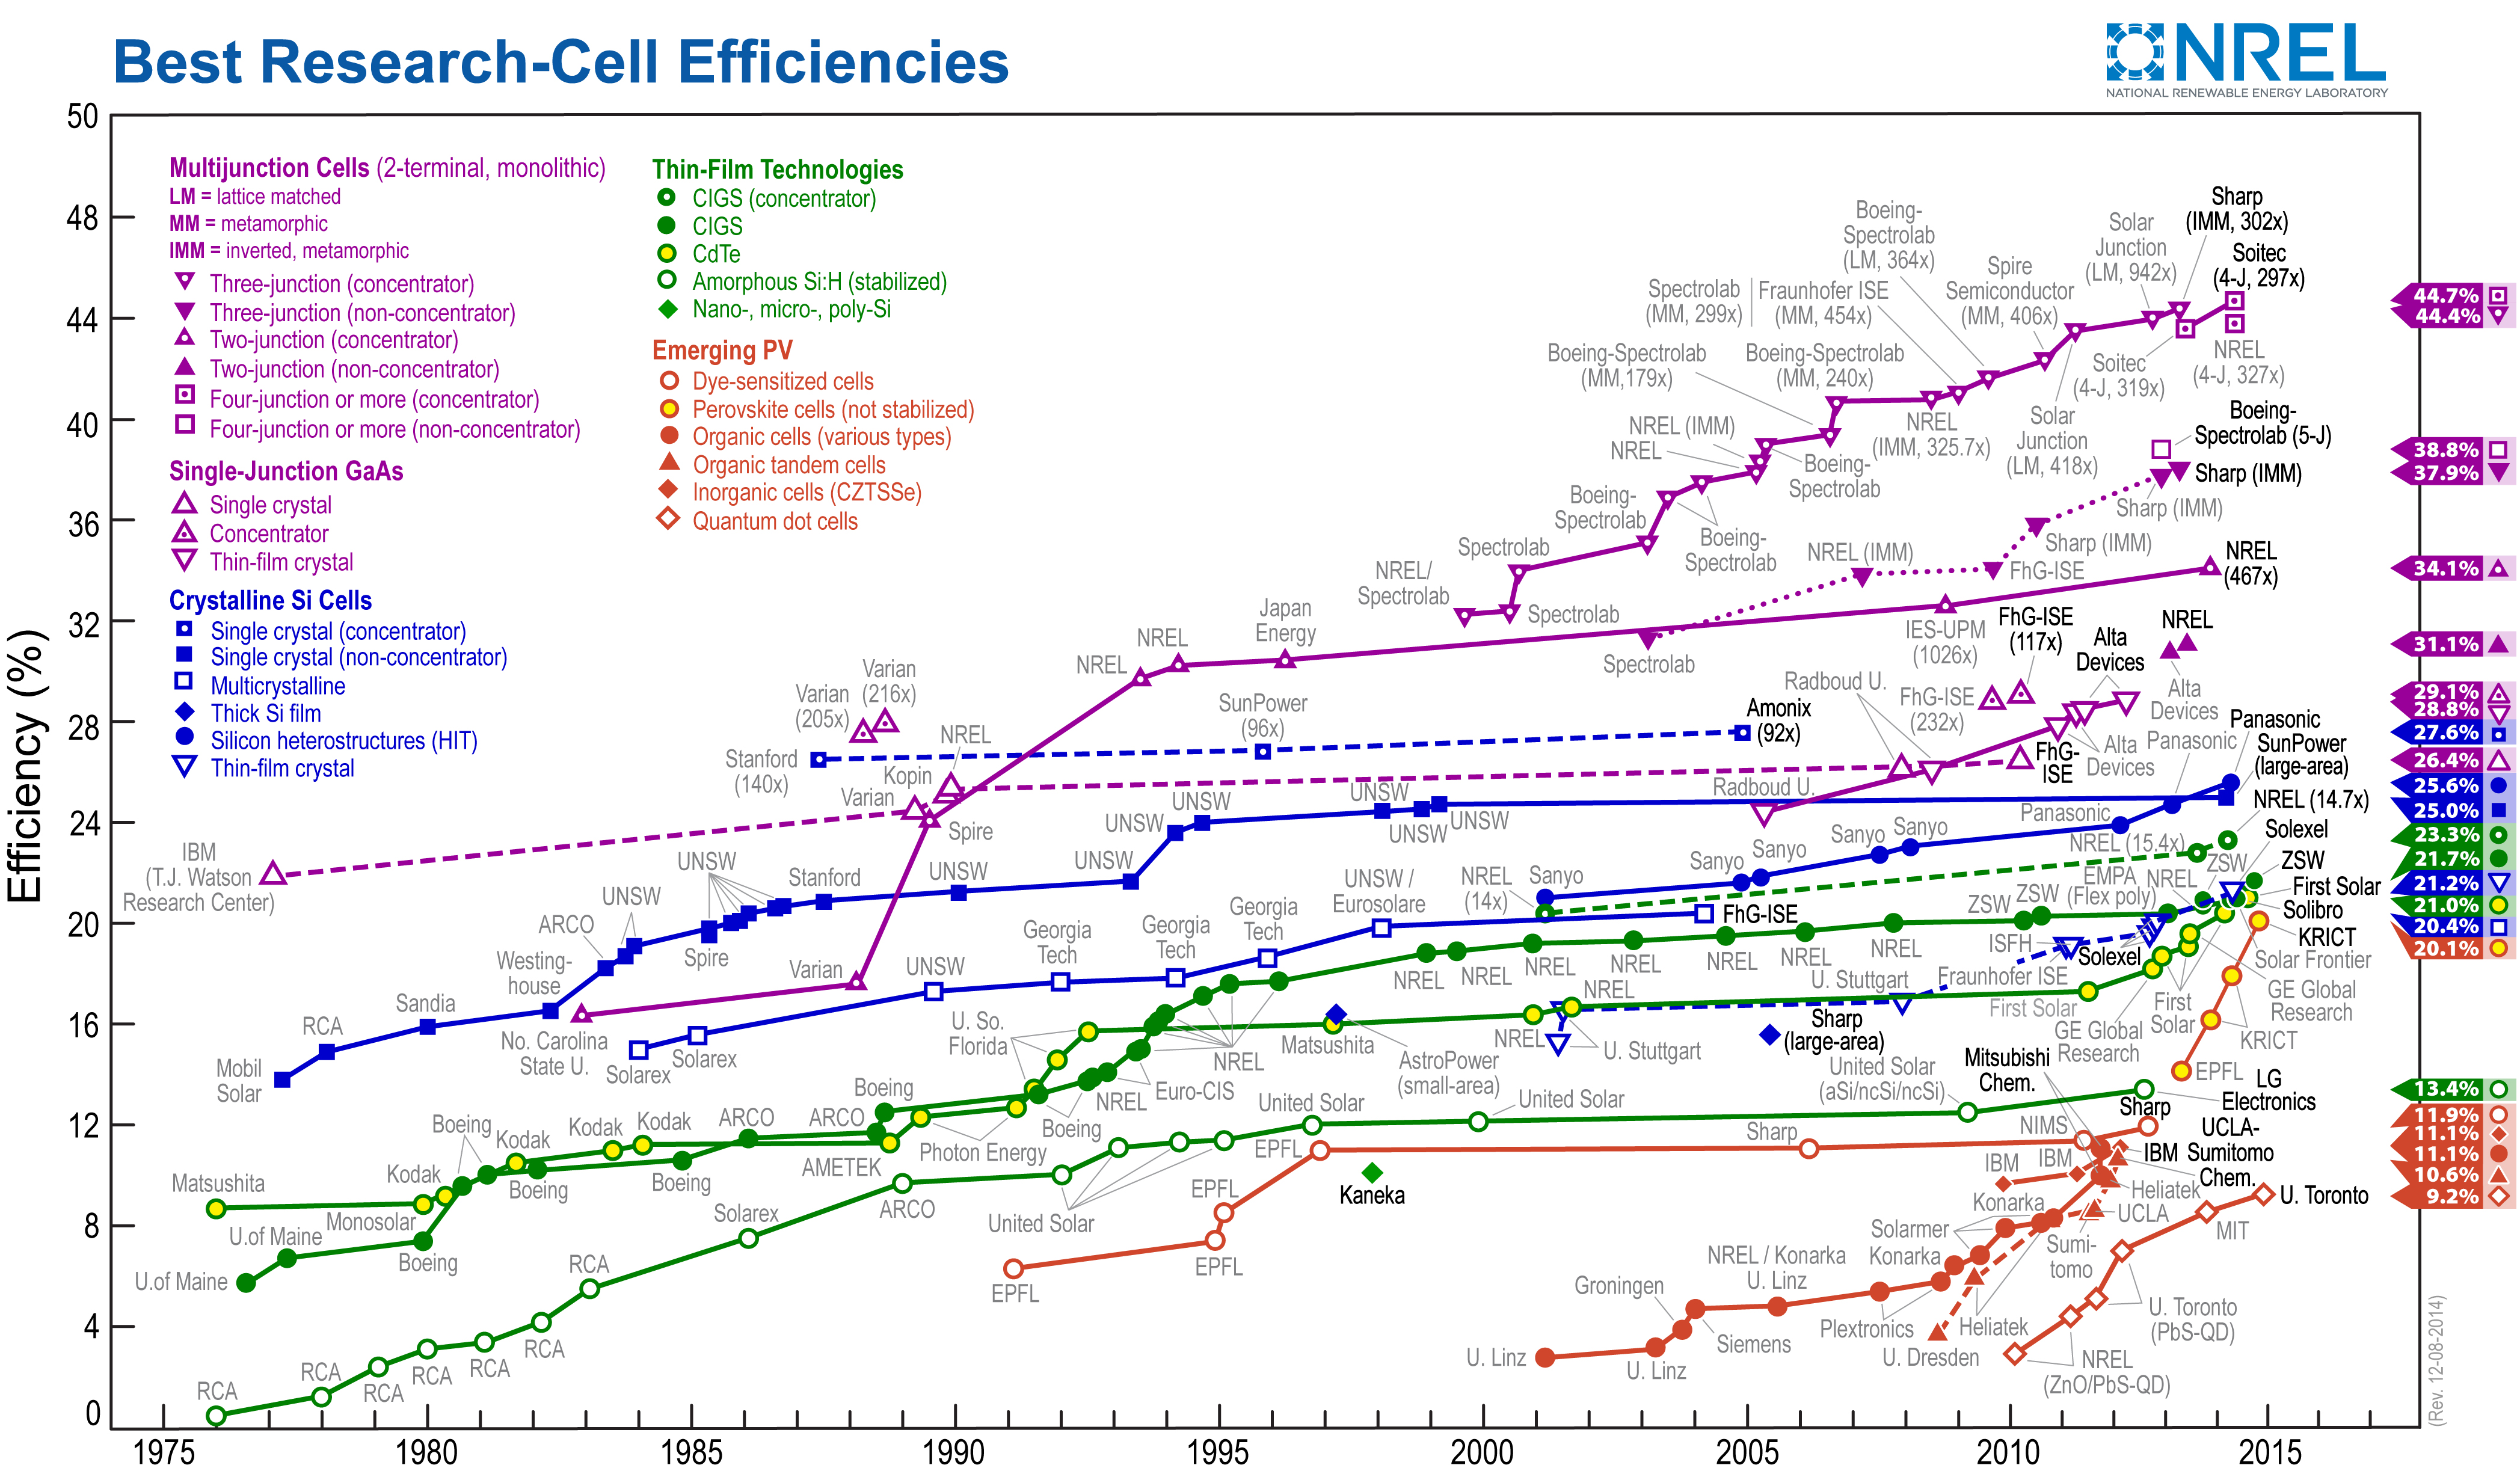
\includegraphics[scale=0.6]{efficiency_chart.jpg}
\caption{Best research-cell efficiencies. Figure is from national renewable energy laboratory (NREL), U.S.A. \cite{nrel}.}
\label{nrel}
\end{sidewaysfigure}

Multijunction cells are the cells which contain multi $p$-$n$ junctions (or subcells). They have different band-gap for each $p$-$n$ junction.
Therefore, different wavelengths of sunlight are absorbed for each junction. For example, wider band-gap junction is at the front of the cell, which absorbs photons with high energy; the junction with 
low band-gap absorbs photons with relatively low energy. In this configuration, the conversion efficiency is higher than the one of single $p$-$n$ junction, for example, the maximum conversion efficiency is 44.7\% by Soitec \cite{dimroth2014wafer} using 
four-junction or more in \textbf{Fig. \ref{nrel}}. Solar cells based on c-Si are the most widely utilized in the PV industries. It has two types in
c-Si photovoltaics: monocrystalline silicon and multicrystalline silicon. Solar cells based on c-Si have high efficiency, for example, the maximum conversion efficiency is 27.6\% with concentrator 
by Amonix \cite{jones2009new} and maximum 25.6\% without concentrator by Panasonic \cite{panasonic} in \textbf{Fig. \ref{nrel}}. Thin-film solar cells are the cells which are made by depositing one or several thin layers. 
They allow cells to be rather 
flexible and result in lower weight. The maximum conversion efficiency for thin-film solar cells is lower than that for c-Si today, which is 23.3\% using copper indium gallium diselenide (CIGS) with concentrator by NREL \cite{ward2014cu} and 
is 21.7\% without concentrator by the center for solar energy and hydrogen research (ZSW) in Stuttgart \cite{zsw} in \textbf{Fig. \ref{nrel}}. The Emerging PV represents the newest ways to create electricity from
sunlight and potentially with higher conversion efficiency, such as perovskite cells in \textbf{Fig. \ref{nrel}}. The maximum conversion efficiency of perovskite cells already reached 20.1\% in Korea research institute of chemical technology (KRICT)\cite{green2015solar}. 
Perovskite cells jump into the world of solar cells only from 2009 \cite{green2014emergence, mcgehee2014perovskite}, and the conversion efficiency is improved remarkably within 5 years. Certainly, search and optimization 
of alternatively solar cell materials are still an ongoing active area today.


\subsection{Single-junction solar cells}
The $p$-$n$ junction is a fundamental building block of solar cells. Single $p$-$n$ homojunction will be explored in this section. The more detailed information about this topic can be found in Refs. \cite{bok1,sproul2003understanding, neamen2003semiconductor}.

We start from separate pieces of $n$- and $p$-type materials at room temperature (assume that all the donor (acceptor) atoms are positively (negatively) ionized at room temperature). In \textbf{Fig. \ref{dopedmaterials}},
the left panel shows illustration of the $n$- and $p$-type materials. The $n$-type
material has many free negatively charged electrons moving freely inside the material, and there are numbers of positively charged immobile donor ions as well. Similarly, a $p$-type material has many free positively
charged holes moving freely in the material, and there are numbers of negatively charged immobile acceptor ions as well. However, both the $n$- and $p$-type materials are still neutral.
The corresponding Fermi levels are shown on the right panel. The Fermi level ($E_{nf}$) is close to conduction band minimum for the $n$-type material due to the many free 
negatively charged electrons. Conversely, the Fermi level of the $p$-type material ($E_{pf}$) is close to valence band maximum due to the many free positively charged holes.

\begin{figure}[H]
    \begin{center}
           % 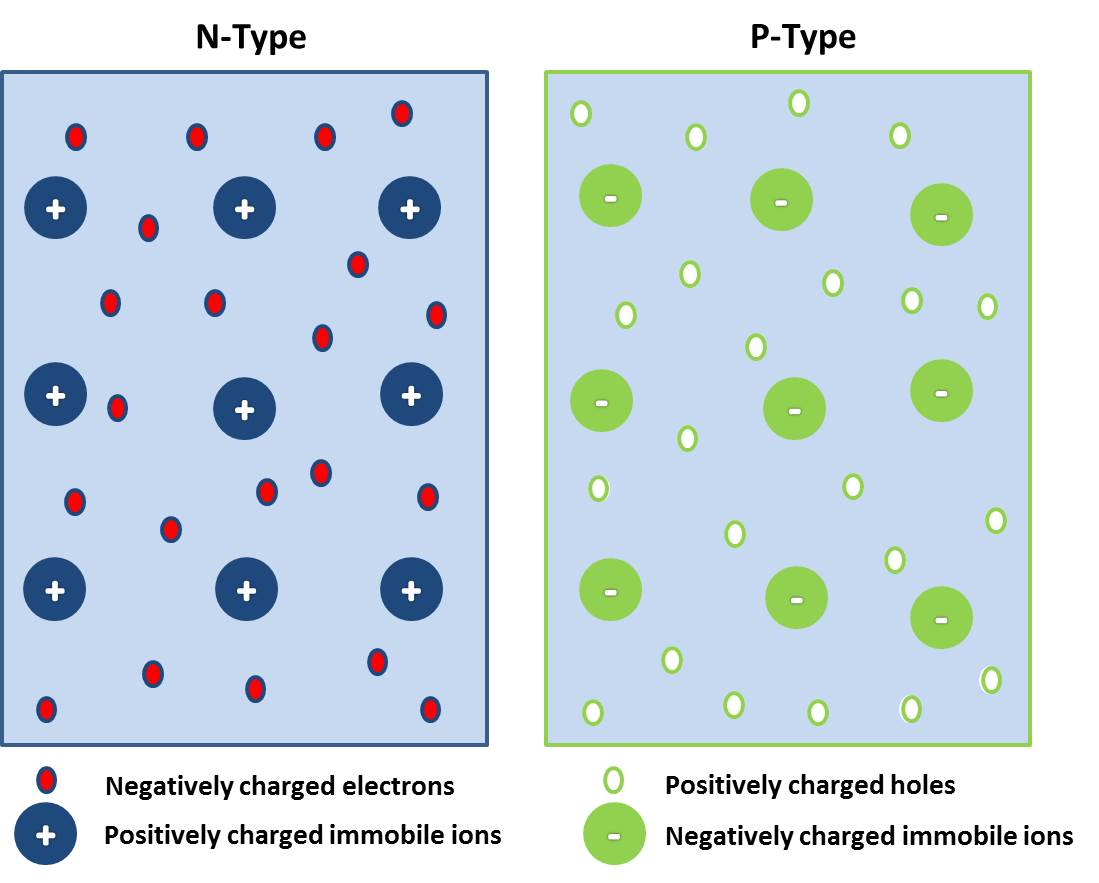
\includegraphics[width=0.4\textwidth,clip]{sepratepn.jpg}
           % 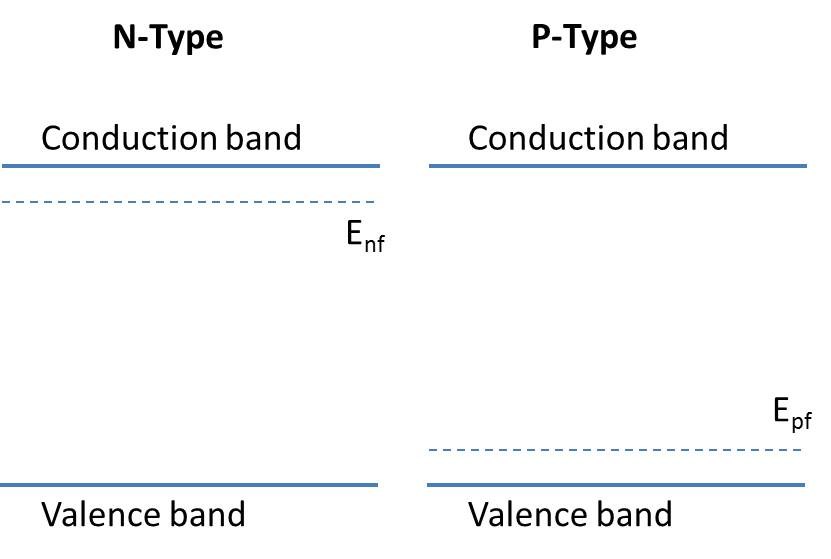
\includegraphics[width=0.4\textwidth,clip]{sepratepn1.jpg}
            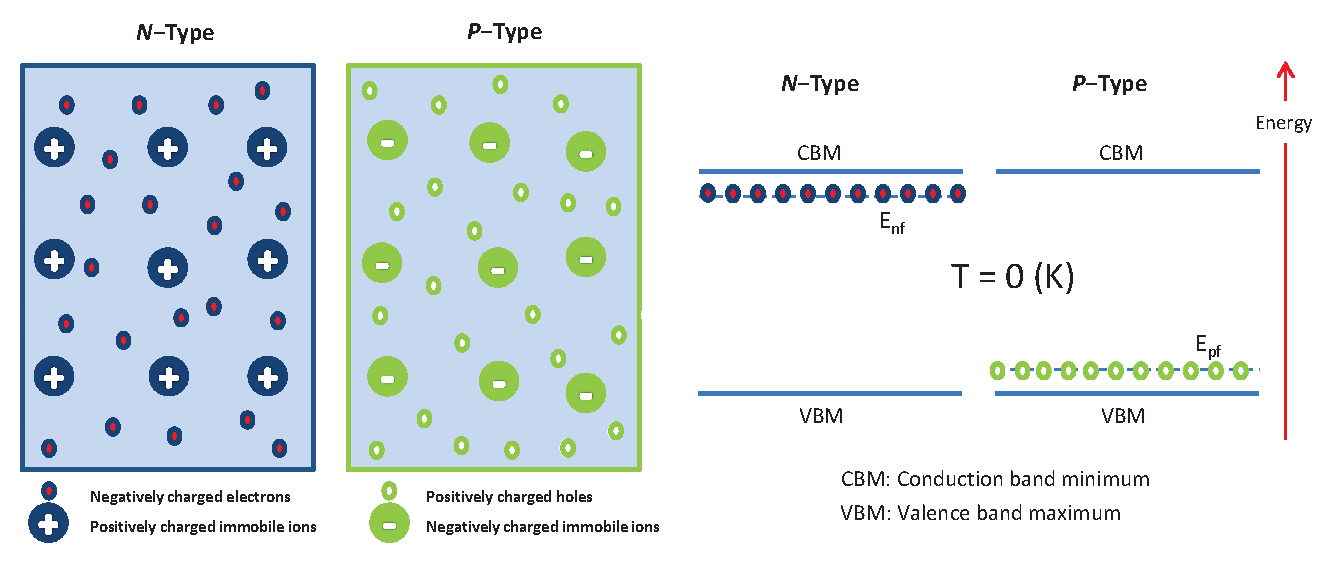
\includegraphics[width=0.8\textwidth,clip]{sepratepn.eps}
     \end{center}
    \caption{Left panel: Doped ($n$-type and $p$-type) materials in dark at room temperature. Right panel: Energy band diagram of $n$- and $p$-type materials in dark at room temperature for two-level model. Assume that all the donor (acceptor) atoms are 
    positively (negatively) ionized at room temperature.}      
    \label{dopedmaterials}
\end{figure}

If the $n$-type and $p$-type materials are joined, the free electrons (holes) in the $n$-type ($p$-type) material will diffuse into the $p$-type ($n$-type) material due to the
lower concentrations of electrons (holes) in the $p$-type ($n$-type) material (\textbf{Fig. \ref{pnjunction}}). In a region, which is near the interface between the $n$- and $p$-type materials, the ionized donor and acceptor ions create a
"build in" electric field which points from the $n$-type material to the $p$-type material. This causes the drift of carriers in the opposite direction. The "build-in" electric field forces the electrons (holes) back into
the $n$-type ($p$-type) material. At certain point, 
the whole material can reach a stable equilibrium due to the achieved balance between diffusion and drift. Formation of the "build-in" electric field is rather important for solar cells, even though there is no current in 
the material so far. In the following text, the region which forms the "build-in" electric field is also called space charge region (SCR). The different Fermi levels for the $n$-type and $p$-type materials become
equal at the stable equilibrium. Therefore, the energy bands bend over and create a potential barrier near the junction (right panel in \textbf{Fig. \ref{pnjunction}}). At last, there is an internal potential V\textsubscript{bi}
in the junction, which can block the diffusion.

\begin{figure}[H]
    \begin{center}
           % 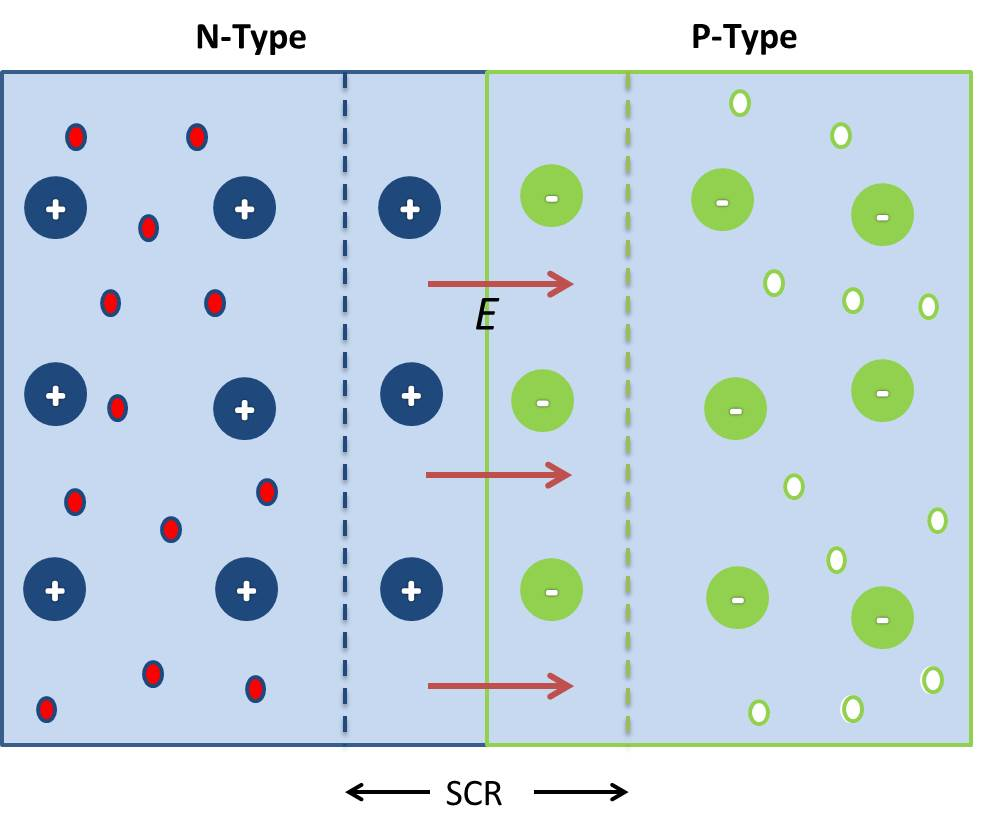
\includegraphics[width=0.4\textwidth,clip]{pnjunction.jpg}
           % 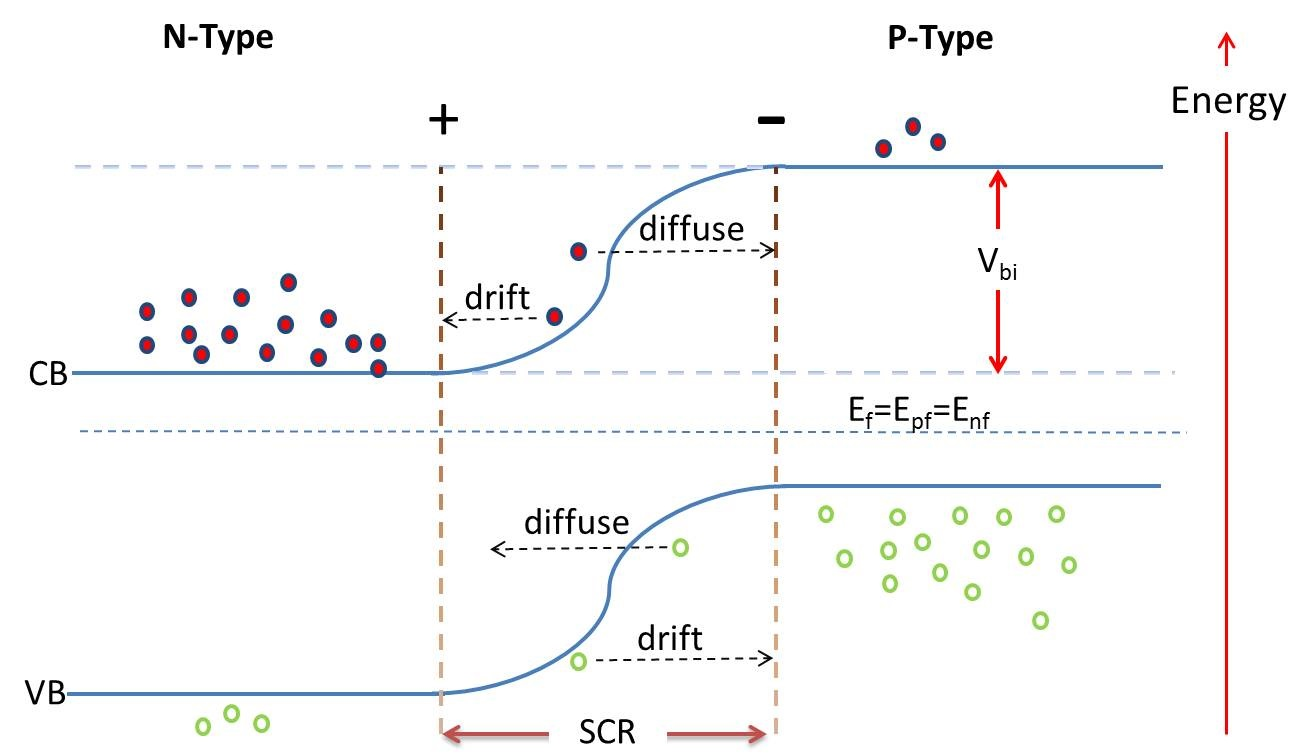
\includegraphics[width=0.5\textwidth,clip]{pnjunction1.jpg}
            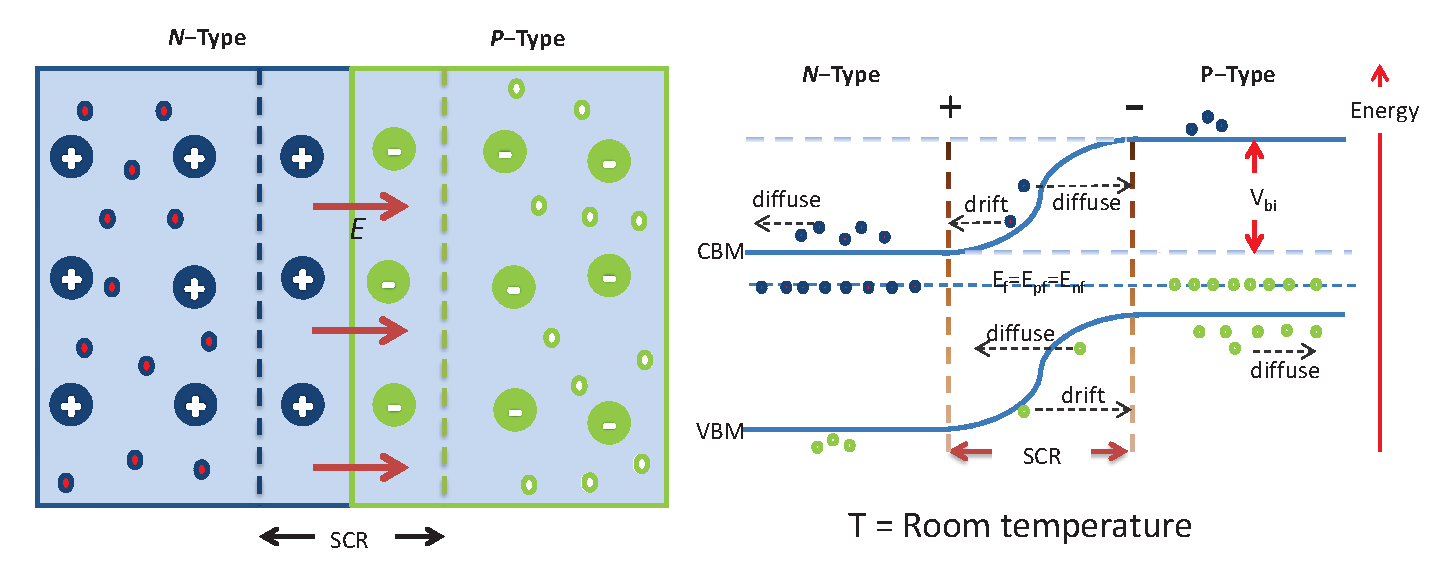
\includegraphics[width=0.7\textwidth]{pnjunction.eps}
     \end{center}
    \caption{Left panel: The $p$-$n$ homojunction in dark at room temperature. Right panel: Energy band diagram of the $p$-$n$ homojunction at the equilibrium in dark at room temperature for two-level model. }      
    \label{pnjunction}
\end{figure}

The $p$-$n$ junction cell with and without illumination are discussed in \textbf{Fig. \ref{illu}} and \textbf{Fig. \ref{illu1}}. If there was a wire with certain resistance connecting 
the $n$- and $p$-type materials, there is no current in the wire under the condition of dark (no illumination). However, if the light shines on the cell, a current can be generated from the $p$-type
to the $n$-type side (conventional current). The reason is that pairs of electron-hole are generated inside the $p$-$n$ junction cell. At the same time, recombination of the paired electron-hole occurs. The rate of paired
electron-hole generation is faster than that of recombination for paired electron-hole. Therefore, net current occurs. Apparently, there are three regions in the whole junction cell where the electrons goes from VBs to CBs, the $n$-type region, the $p$-$n$
junction, and the $p$-type region. In the either $n$- or $p$-type region (especially, region which is far away SCR), the electron–hole pair only exists for a short time,  and it is most probable that electrons
will jump down from CBs to VBs again. However, the electron-hole pair can be separated in the $p$-$n$ junction region due to the "build-in" electric field. Therefore, current is generated. Actually, the electron-hole pair in
the either n- and p-type material (especially, for them which are near SCR) also have the chance to diffuse into the SCR, which can contribute to generate current or to reduce current.

\begin{figure}[H]
\centering
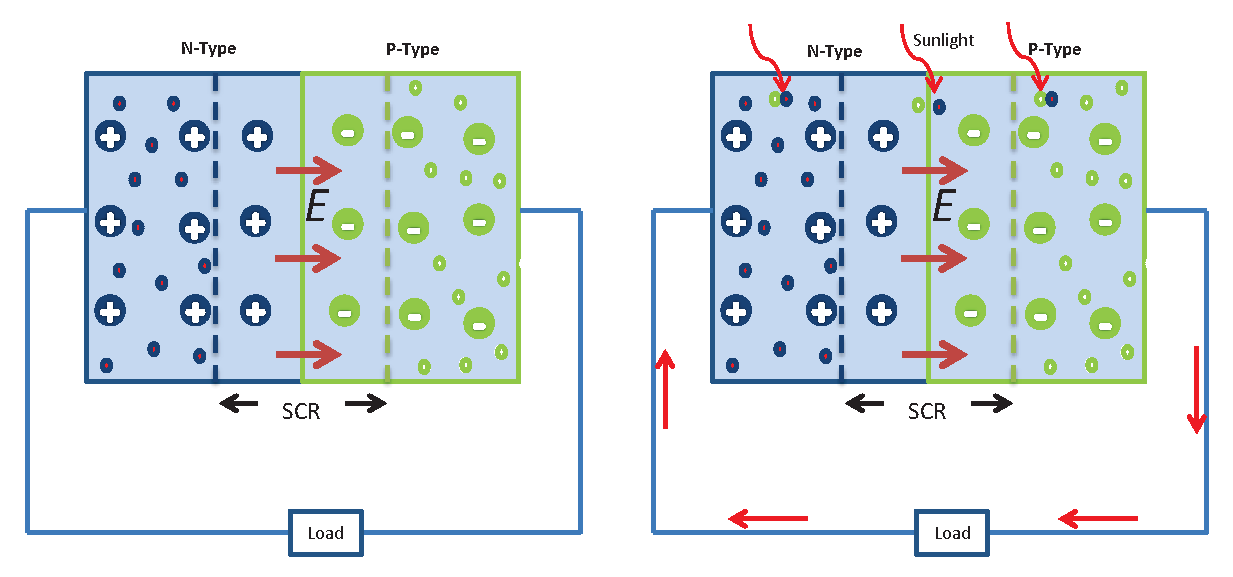
\includegraphics[scale=0.5]{illumination.eps}
\caption{Left panel: the $p$-$n$ homojunction at dark with load. Right panel: the $p$-$n$ homojunction under illumination with load at room temperature.}
\label{illu}
\end{figure}

In \textbf{Fig. \ref{illu1}}, the SCR becomes more "smooth" due to the extra load, such as light bulb. It is equivalent to apply external potential. The stabilized Fermi level at a stable equilibrium splits under illumination.
The chemical potential ($\bigtriangledown \mu$) is created, which is considered as the electron charge times the voltage across the device. The generation and recombination by impurities are not analyzed in here.

\begin{figure}[H]
\centering
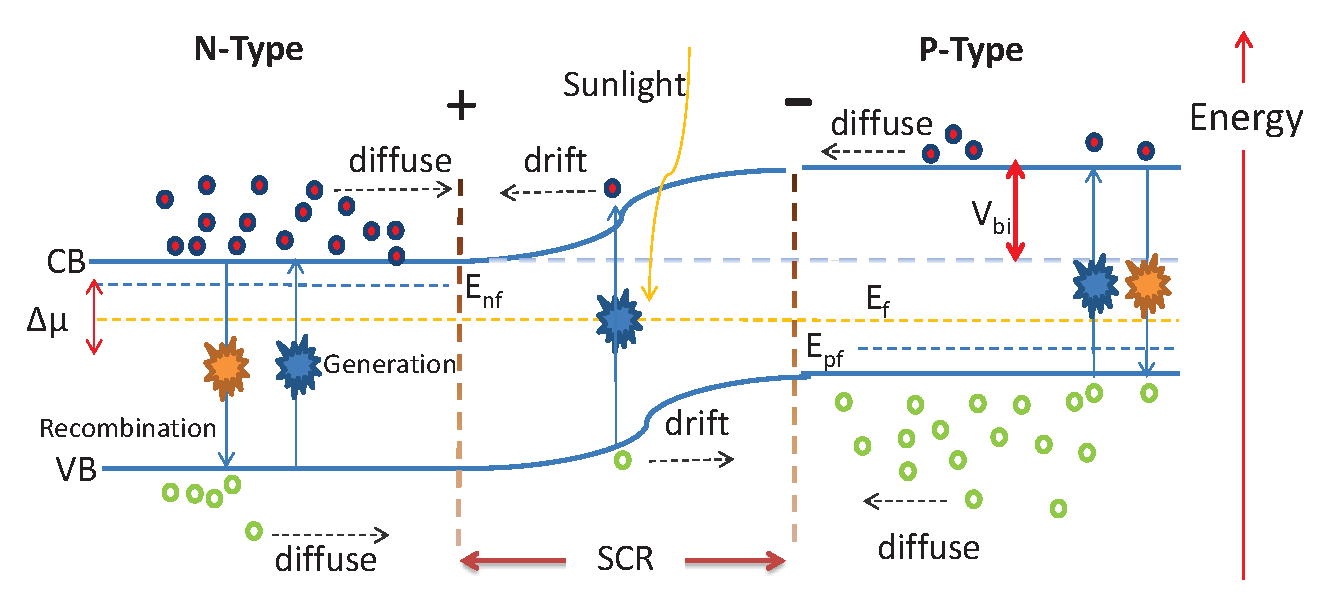
\includegraphics[scale=0.5]{illumination1.eps}
\caption{Energy band diagram of the $p$-$n$ homojunction under illumination with load for two-level model.}
\label{illu1}
\end{figure}


Current-voltage characteristic is defined in \textbf{Fig. \ref{ivcharac}} with some important parameters of solar cells. $V_{oc}$ and $I_{sc}$ are the open circuit voltage (the maximum voltage) and short circuit current
(maximum current), respectively. $V_{mp}$ and $I_{mp}$ are the voltage and current, respectively,  which yield the maximum power. The maximum power generated by solar cells
is $P_{out}=V_{mp} \times I_{mp}$. That is the rectangle bounded by dashed lines in \textbf{Fig. \ref{ivcharac}}. 

\begin{figure}[H]
\centering
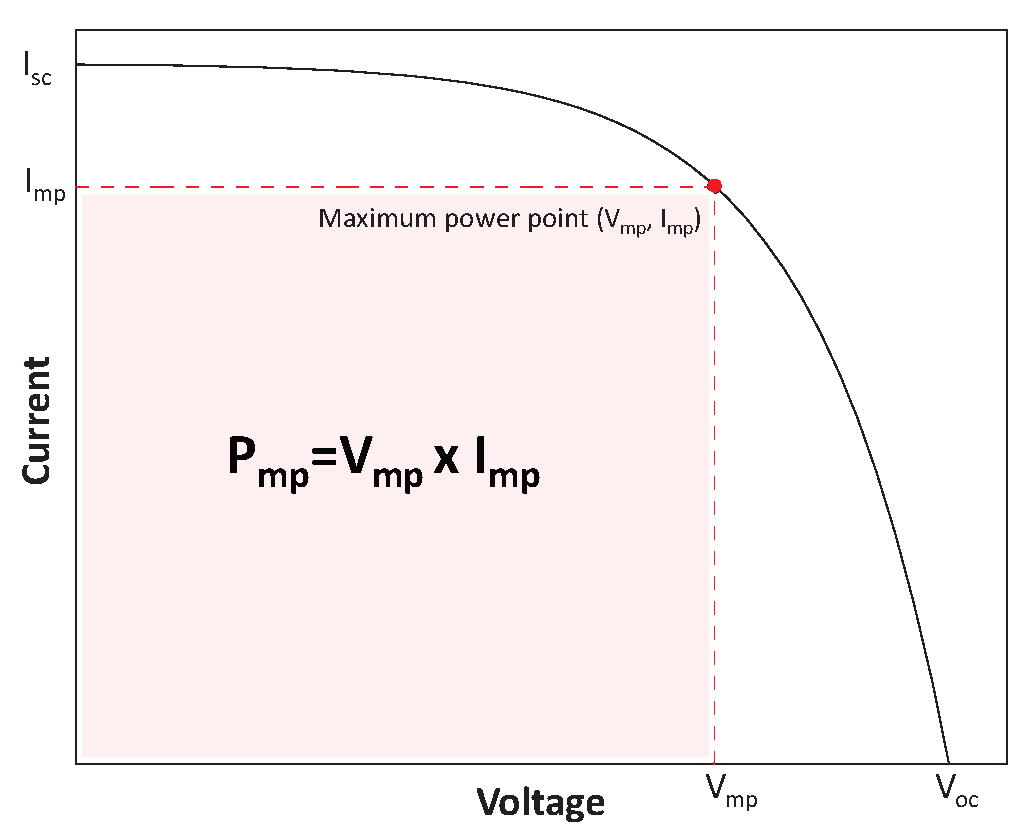
\includegraphics[scale=0.5]{IV.eps}
\caption{Current-voltage characteristic of a solar cell under illumination.}
\label{ivcharac}
\end{figure}


Solar cell performance is often represented by fill factor ($FF$) and power conversion efficiency ($\eta$):

\begin{equation}
FF = \frac{P_{out}}{V_{oc} \cdot I_{sc}} = \frac{V_{mp} \cdot I_{mp}}{V_{oc} \cdot I_{sc}}
\end{equation}

\begin{equation}
\eta = \frac{P_{out}}{P_{in}} = \frac{FF \cdot V_{oc} \cdot I_{sc}}{P_{in}}.
\end{equation}


Here, $P_{in}$ is incident photon power per second. Conversion efficiency of solar cells is proportional to the $FF$, $V_{oc}$, and $I_{sc}$. There are several aspects affecting
the conversion efficiency. The $V_{oc}$ is directly proportional to band-gap of a material, and the $I_{sc}$ is proportional to number of absorbed photons. When band-gap is decreased, more spectrum of sunlight can be absorbed.
However, the $V_{oc}$ will be reduced in this case. More importantly, excess energy of photons is lost due to thermalization in solar cells. When band-gap is increased, more transparency loss from photons with energy lower than
the band-gap occurs. One can find more detailed analysis of conversion efficiency in Ref. \cite{bok1}.


\section{Solar cell materials}

In 1839, French physicist A. E. Becquerel \cite{Becquerel} revealed the photovoltaic effect for the first time. Charles Fritts built the first solid state photovoltaic (PV) cell using semiconductor selenium in 
1883 \cite{etgar2013semiconductor,gourdin2007solar}. It is not until 1941 that
the first silicon-based solar cell was demonstrated \cite{1941ohl1, 1941ohl2}. Today, there are many different types of solar cell materials. The reason why the best solar cell material is not found yet is that it is expected to be not only high efficiency but 
also environmentally friendly, and low cost. It requires not only that the growth and manufacturing process of solar cell materials should be cheaper, but also that the devices should have longer application life. Moreover, the raw material
should be abundant and non-toxic as well. In this section, four main solar cell materials are discussed briefly: silicon (Si), gallium arsenide (GaAs), cadmium telluride (CdTe), copper indium gallium diselenide (CIGS).

Potential solar cell materials need to fulfill several properties, such as large absorption coefficient and a band-gap energy between 0.7 to 2.0 eV. Under these conditions, many materials can be found.
However, other properties are needed to be considered as well, such as cost and environmental safety. Thereby, only part of them are suitable to be utilized in reality.

\begin{figure}[H]
\centering
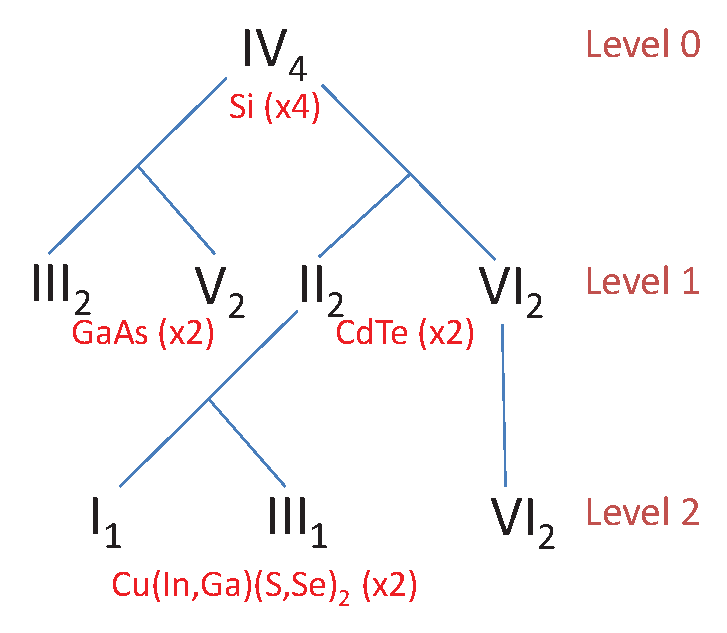
\includegraphics[scale=0.5]{tree.eps} 
\caption{Tree of tetragonal bonded semiconductor, the roman numerals mean group numbers in the chemical element periodic table, and the subscript implies number of elements.}
\label{lscm}
\end{figure}

In \textbf{Fig. \ref{lscm}}, formation of tetragonal semiconductors is considered as a series of cation mutations where total number of valence electrons is the same and it keeps the charge neutral in the compound \cite{chen2009electronic, chen2009crystal, walsh2009design}. For example, group number
IV element Si (level 0) with four 4\textsuperscript{+} ions is equivalent to two 3\textsuperscript{+} ions and two 5\textsuperscript{+} ions, such as GaAs (level 1). It is also equivalent to two 2\textsuperscript{+} ions
and two 6\textsuperscript{+} ions, such as CdTe (level 1). The CIGS can be derived applying the same process on group number II element on the level 1 in \textbf{Fig. \ref{lscm}}. This method was suggested by Goodman and Pamplin 
\cite{goodman1958prediction, pamplin1964systematic}. 



\subsection{Crystalline silicon solar cells}
Solar cells based on Si dominate solar power world today, which account for more than 90\% of total PV market \cite{hoffmann2006pv}.
Different forms of Si are used in this kind of solar cells, that is, monocrystalline Si and polycrystalline Si. 
The success of Si is due to a number of reasons. For example, over 90\% in the crust of earth is composed of silicate minerals, which yields huge available Si. Moreover, it has higher conversion efficiency, and it is also proved that 
it has excellent stability and reliability under outdoor conditions. However, Si also has drawbacks. It has an indirect band-gap, hence it has a lower optical absorption coefficient. In order to absorb incident sunlight fully, 
thicker Si (wafer) (around \SI{0.2} {\milli\meter}) is required \cite{brewer2013renewable}. c-Si has to be high quality and defect free in order to avoid losing the carriers before collection. Last but not least, it is expensive to purify the Si from the silicate minerals, which
limits the cost reduction of wafer-based Si technology. 

However, solar cells based c-Si technology are still leading the market of solar cells since many companies are trying to lower the cost in the whole manufacture.



\subsection{Gallium arsenide}
GaAs has a zinc blende crystal structure with a direct band-gap around 1.5 eV at room temperature \cite{cardona2005fundamentals, madelung1996semiconductors, madelung2004semiconductors}. Some electronic properties of GaAs
are superior to Si, such as higher electron 
mobility, higher saturated electron velocity, and absorb sunlight more efficiently due to the direct band-gap. The optimum band-gap for a single junction solar cells is suggested around 1.3 eV by theoretical calculation 
from Henry (1980) \cite{henry1980limiting}, who modified the original Shockley-Queisser limit \cite{shockley1961detailed}. Therefore, one of the applications of GaAs is solar cells. GaAs has been extensively researched
since 1950s, and the first GaAs solar cell was established in
1970 by Zhores Alferov's team \cite{alferov2001nobel}. Today, the conversion efficiency for single junction solar cells based on GaAs is 28.8\% \cite{yablonovitch2012opto}. However, the
price of solar cells based on GaAs is more expensive in comparison with the price of solar cells based on Si.
Researches are focusing on how to reduce the price today, and the main application of solar cells based on GaAs is in the space application. However, the arsenic toxicity should be considered as the main disadvantage of this kind of 
solar cells. 

The conversion efficiency of 44.7\% for four-junction GaInP/GaAs/GaInAsP/GaInAs concentrator solar cells was achieved by Soitec on March 2014 \cite{dimroth2014wafer}.

\subsection{Thin-film materials}

Thin-film solar cells have several layers of thin-film with total thickness less than \SI{10} {\micro\meter} \cite{maissel1995handbook}. The cost of this kind of solar cells can potentially be reduced since less materials are utilized to make thin-film solar cells. The development of thin-film
solar cells was started since 1970s. Currently, the maximum conversion efficiency for thin-film is 23.3\% \cite{ward2014cu}. Three different thin-film
materials are discussed in this section: amorphous silicon (a-Si), cadmium telluride (CdTe), and copper indium gallium diselenide (CIGS).

The a-Si is the first thin-film solar cell material reaching the large-scale production \cite{carlson1976amorphous, street2000technology, schropp1998amorphous}. It has higher absorption coefficient than that of c-Si. Therefore, the thickness can be less than \SI{1} {\micro\meter}. The 
main disadvantages a-Si solar cells is the lower conversion efficiency, the actual conversion efficiency for commercial single junction solar cells based on a-Si is between 4\% and 8\% \cite{irena}. This limits the development of a-Si thin-film solar cells.
a-Si solar cells are suited to the situations which require low cost over high efficiency. 

CdTe was first reported in the 1960s \cite{wolden2011photovoltaic}. However, it was not developed rapidly until in the early 1990s. CdTe has a number of advantages as an absorber. It has higher absorption coefficient. The band-gap is around 1.45 eV, which 
is very near the optimum value for single-junction solar cells. The manufacturing process is easier to control, which results in the cost of manufacture is low \cite{meyers1988design}. Moreover, the conversion efficiency of 
commercial modules already reached 17\% \cite{firstsolarcdte}.
However, an important question should be considered in order to large-scale CdTe manufacture: cadmium toxicity and tellurium availability. 

CIGS is a direct band-gap semiconductor with high optical absorption coefficient. It is seen as one of the most promising solar cell materials for the near future. It is always employed in a heterojunction structure, mainly it is with the thinner
$n$-type CdS layer \cite{green2007thin}. The 23.3\% CIGS world record conversion efficiency was achieved in the laboratory \cite{ward2014cu}. The interesting part is that it can be alloyed by the ratio of Ga/(Ga+In), and the band-gap can be tuned along with that. The band-gap 
is between 1.0 eV and 1.7 eV for this kind of alloy \cite{kumar2013cation, chen2012band, chen2011parameterization, persson2009impurity, green2006third}. CIGS does not contain any toxic element.

%\section{CuIn\textsubscript{1-\textit{x}}Ga\textsubscript{\textit{x}}Se\textsubscript{2}(CIGS) materials}
\section{Copper indium gallium diselenide (CIGS)}
CIGS is a chalcopyrite-type material, which is considered as one of the most promising thin-film solar cell materials. 
CuInSe\textsubscript{2} was first synthesized by Hahn in 1953 \cite{ZAAC}. It was first exploited as an absorber material in a single crystal solar cell in 1974 \cite{CuInSe21974}, and the conversion efficiency is around 
5\%. The first thin-film solar cell based on CuInSe\textsubscript{2} and CdS was invented by Kazmerski \cite{kazmerski1976thin}. During the 1980s, Boeing Corporation did much research on the thin-film polycrystalline CIGS solar cells. 
To date, the highest conversion efficiency in laboratory situation for the solar cells based on CIGS is 23.3\% \cite{ward2014cu}.


\subsection{Crystal structure}
Crystal structure of CIGS can be derived from zinc blende crystal structure of zinc selenide (ZnSe). In \textbf{Fig. \ref{crystal_cigs}}, the crystal structures of ZnSe and CuInSe\textsubscript{2} are presented. 
Atoms Zn are replaced by atoms Cu and In or Ga in the zinc blende of ZnSe. It requires to double the unit cell of ZnSe in the $z$-direction. The lattice parameter $c$ for CIGS is not exact 2$a$ normally, because bond 
strength and lengths between Cu-Se and In-Se or Ga-Se are different \cite{chen2009crystal}.

Chalcopyrite CuInSe\textsubscript{2} and CuGaSe\textsubscript{2} have space group $D_{2d}^{12}$ ($I\overline{4}2d$; space group no. 122).
The conventional unit cell has four copper (Cu) atoms on Wyckoff position 4$a$ ($S_4$ point-group symmetry), four indium (In) or gallium (Ga) atoms are on position 4$b$ ($S_4$ point-group symmetry),
and eight selenium (Se) atoms are on position 8$d$ ($C_2$ symmetry). 
The Se 8$d$ positions are fully defined with the position ($x$, $y$, $z$), and each anion Se atom has two inequivalent bonds $\delta$(Cu–Se) and $\delta$(In–Se) or $\delta$(Ga–Se) \cite{parlak2006ab, hones2008polarization,persson2008anisotropic}. 
For the CuIn\textsubscript{0.5}Ga\textsubscript{0.5}Se\textsubscript{2}, the structure is chosen so that each Se atom has bonds with two Cu atoms, one In, and one Ga atom. The space group is $S_{4}^{2}$ ($I\overline{4}$; space 
group no. 82) \cite{li2011electronic}.


\begin{figure}[H]
\centering
%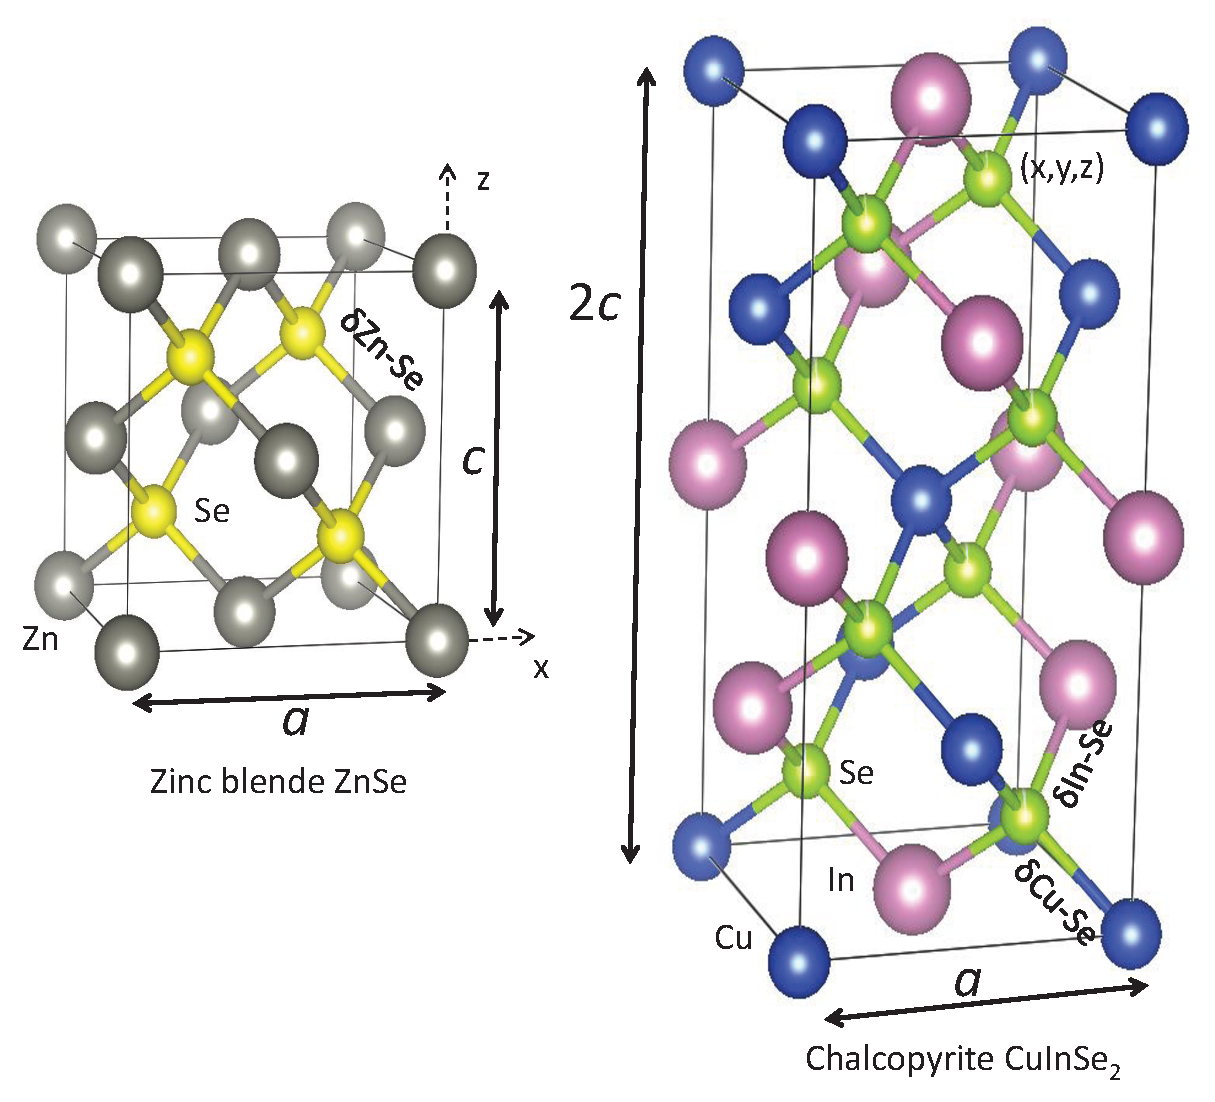
\includegraphics[scale=0.4]{structureciise.eps} 
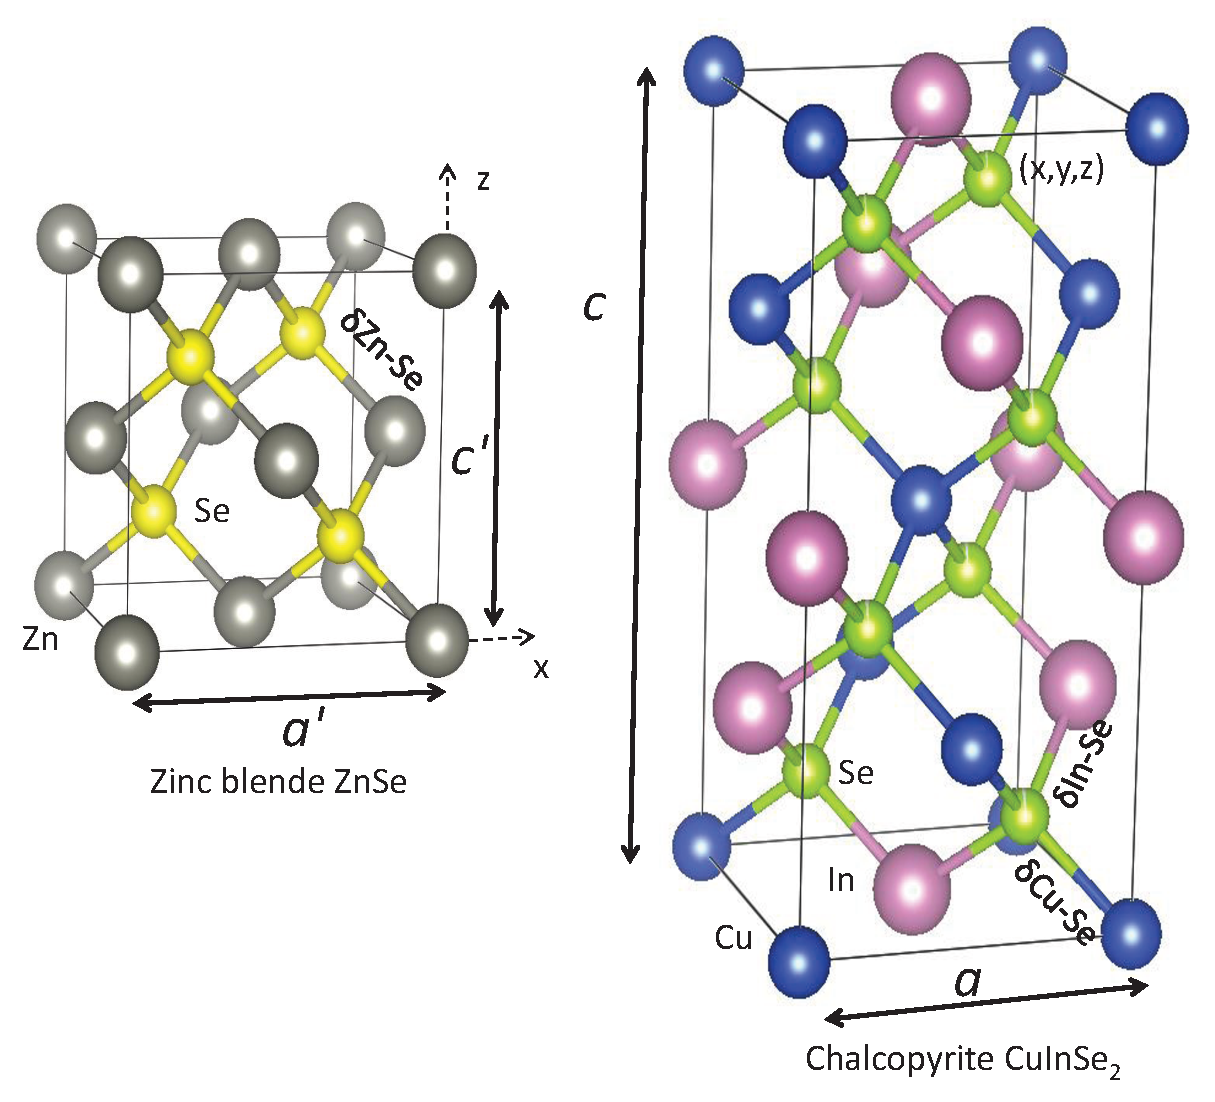
\includegraphics[scale=0.4]{cigscrystalstructure.eps} 
\caption{Crystal structures of zinc blende ZnSe and chalcopyrite CuInSe\textsubscript{2}.}
\label{crystal_cigs}
\end{figure}


\subsection{Optical properties and defects in the CIGS}
CuInSe\textsubscript{2} has a direct band-gap around 1.0 eV, and the absorption coefficient is relatively higher than that of c-Si due to the direct band-gap. The quaternary CIGS alloy will be available by alloying Ga element, while the band-gap is tuned as well from 
1.0 eV to 1.7 eV. The CIGS can be applied as an absorber layer for the thin-film solar cells due to the high absorption coefficient. The band-gap can be approximated by the function of Ga content ($x$) \cite{luque2011handbook}

\begin{equation}
E_g(x) = 1.010+0.626x-0.167x(1-x).
\end{equation}

Alloying the Ga element will decrease the electron affinity of CIGS, which will make conduction bands upward shift. However, the valence bands remain the same positions \cite{jiang2004does}. This also explains the reason why the band-gap increases with 
more Ga element in the CIGS. An overview of the properties of CuInSe\textsubscript{2} and CuGaSe\textsubscript{2} are described in \textbf{Table. \ref{kth518}} 


\vspace{0cm}

\begin {table}[!htb]
\centering
\begin{tabular}{l l l}  
\toprule
\toprule
%\rowcolor[gray]{0.7}
\multicolumn{3}{c}{\large Properties of CuInSe\textsubscript{2} and CuGaSe\textsubscript{2}}  \\  
%\midrule
\cellcolor{blue!25} Properties & \cellcolor{blue!25} CuInSe\textsubscript{2} & \cellcolor{blue!25} CuGaSe\textsubscript{2} \\ 
%\midrule

Space group & $D_{2d}^{12}$(I$-$42$d$), no. 122 \cite{madelung2004semiconductors} & $D_{2d}^{12}$(I$-$42$d$), no. 122 \cite{madelung2004semiconductors}\\ 
%\midrule
\rowcolor[gray]{0.9}
Lattice constants (Å) & $a$ = $b$ = 5.78, $c$ = 11.55 \cite{madelung2004semiconductors} & $a$ = $b$ = 5.61, $c$ = 11.00 \cite{madelung2004semiconductors}\\ 
%\midrule
Wyckoff positions & Cu:4$a$, In:4$b$, Se:8$d$ \cite{parlak2006ab, hones2008polarization,persson2008anisotropic}& Cu:4$a$, Ga:4$b$, Se:8$d$ \cite{parlak2006ab, hones2008polarization,persson2008anisotropic}\\ 
%\midrule
\rowcolor[gray]{0.9}
Direct band-gap (eV) & $E_g$ = 1.01 \cite{madelung2004semiconductors} & $E_g$ = 1.68 \cite{madelung2004semiconductors}\\ 
%\midrule
Effective masses on  & Electrons: 0.08 \cite{rau2006wide}& Electrons: 0.14 \cite{rau2006wide} \\ 
 $\Gamma$ point (m\textsubscript{0})                                     & Holes(heavy): 0.71 \cite{rau2006wide}& Holes(heavy): 1.2 \cite{rau2006wide} \\ 
\rowcolor[gray]{0.9}
Main intrinsic defects & $n$-type: V\textsubscript{Se}; In\textsubscript{Cu} \cite{chen2010intrinsic, schuler2004self, lany2008intrinsic, zhang1998defect}&  $n$-type: V\textsubscript{Se}; Ga\textsubscript{Cu} \cite{chen2010intrinsic, schuler2004self, lany2008intrinsic, zhang1998defect}\\
\rowcolor[gray]{0.9}   & $p$-type: V\textsubscript{Cu}; Cu\textsubscript{In} \cite{chen2010intrinsic, schuler2004self, lany2008intrinsic, zhang1998defect}&  $p$-type: V\textsubscript{Cu}; Cu\textsubscript{Ga} \cite{chen2010intrinsic, schuler2004self, lany2008intrinsic, zhang1998defect} \\  
%\midrule
Crystal field splitting (eV)& 0.006 \cite{madelung2004semiconductors} & $-$0.10 \cite{madelung2010springer}\\ 
%\midrule
\rowcolor[gray]{0.9}
Spin-orbit splitting (eV) & 0.23 \cite{madelung2004semiconductors}& 0.238 \cite{madelung2004semiconductors} \\ 
%\midrule
Dielectric constants $\varepsilon(0)$ & 15.7 \cite{madelung2004semiconductors} & 11.0 \cite{rau2006wide}\\
%\midrule
\rowcolor[gray]{0.9}
Melting temperature (K)& 1260 \cite{madelung2004semiconductors} & 1310 $-$ 1340 \cite{madelung2004semiconductors}\\
%\midrule
Thermal expansion & a axis: 11.23$\times$10\textsuperscript{$-$6} \cite{madelung2004semiconductors}& a axis: 13.1$\times$10\textsuperscript{$-$6} \cite{madelung2004semiconductors}\\
 coefficients (1/K) & c axis: 7.90$\times$10\textsuperscript{$-$6} \cite{madelung2004semiconductors}&c axis: 5.2$\times$10\textsuperscript{$-$6} \cite{madelung2004semiconductors}\\ 
%\midrule
\rowcolor[gray]{0.9}
Thermal conductivity& 0.086 \cite{neumann1986optical} & 0.129 \cite{madelung2004semiconductors} \\ 
 \rowcolor[gray]{0.9} W/(cm $\times$ K)&  & \\ 
\bottomrule
\end{tabular}
\caption {Properties of CuInSe\textsubscript{2} and CuGaSe\textsubscript{2}.}
\label{kth518}
\end{table}


%The main native defects in CIGS \cite{chen2010intrinsic, schuler2004self, lany2008intrinsic, zhang1998defect} include <2V\textsubscript{Cu}, In\textsubscript{Cu}>, <Cu\textsubscript{In}, In\textsubscript{Cu}>, V\textsubscript{Cu}, In\textsubscript{Cu}, Cu\textsubscript{In} V\textsubscript{Se} and Ga\textsubscript{Cu}.

CIGS is a non-stoichiometric compound, and the high quality thin-film solar cells mainly employ Cu-poor (Cu: 22.5$-$24.5\%) high off-stoichiometric CIGS absorber.
V\textsubscript{Cu} is the most important native defect in CIGS due to the low formation energy. Therefore, CIGS can be grown $p$-type easily under the condition of V\textsubscript{Cu}.
There are some extrinsic divalent cation donors as well, such as Zn\textsubscript{Cu}, Cd\textsubscript{Cu}, and Cl\textsubscript{Se}. The formation energies 
for them are relatively low for CIS and CuGaSe\textsubscript{2} (CGS). In fact, CIS is possible to be $n$-type as well. However, CGS is not possible to be $n$-type under equilibrium conditions. The reason is that the low formation energy of
V\textsubscript{Cu} limits the possibility of achieving electronic $n$-type character, especially in Ga-rich CIGS \cite{persson2005n, zhao2004can}. This may also explains why the best solar cell is with 
the Ga content of 30\% (x = 0.3), however,
the band-gap energy of the CIGS suggests that the optimum solar cell conversion efficiency is obtained with x between 0.5 and 0.7.


\subsection{CIGS solar cell structure}

The solar cells device based on CIGS is a heterojunction device, which normally has five thin-film layers with different functional properties \cite{lundberg2005effect, lundberg2003diffusion, ramanathan2003properties}.
A schematic of conventional device structure is shown in  \textbf{Fig. \ref{device}}

\begin{figure}[H]
\centering
%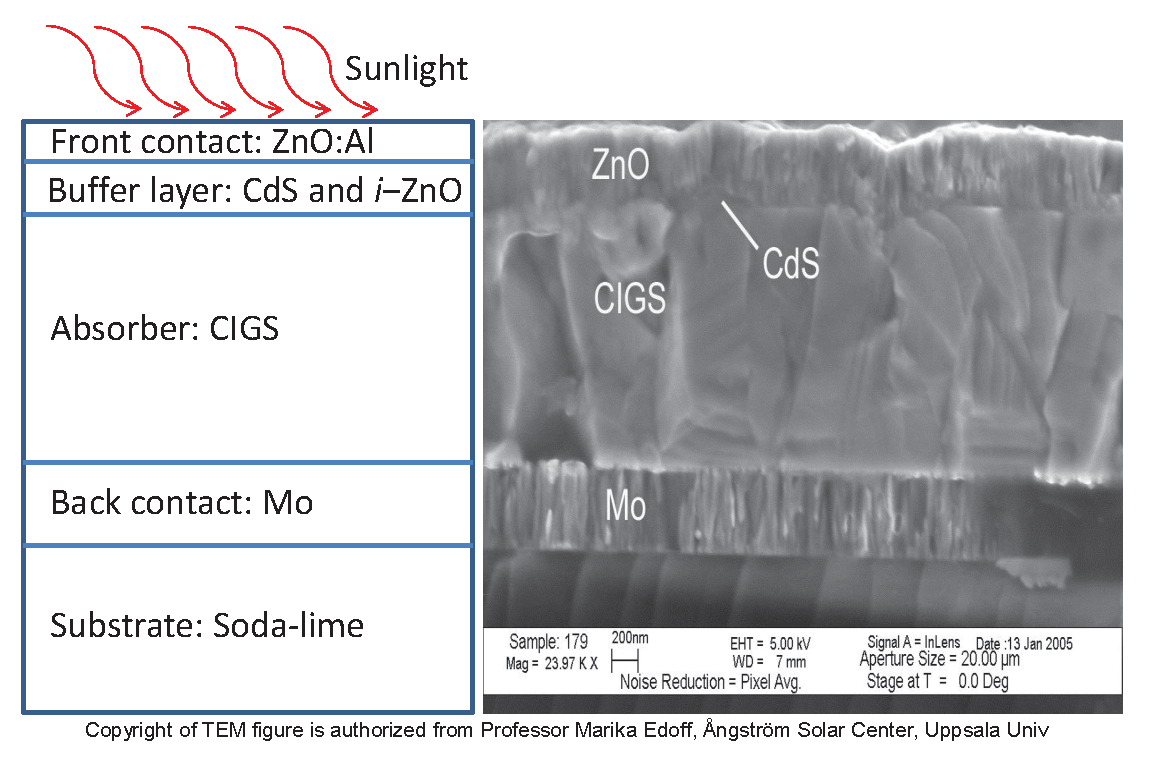
\includegraphics[scale=0.5]{devicestruc.eps} 
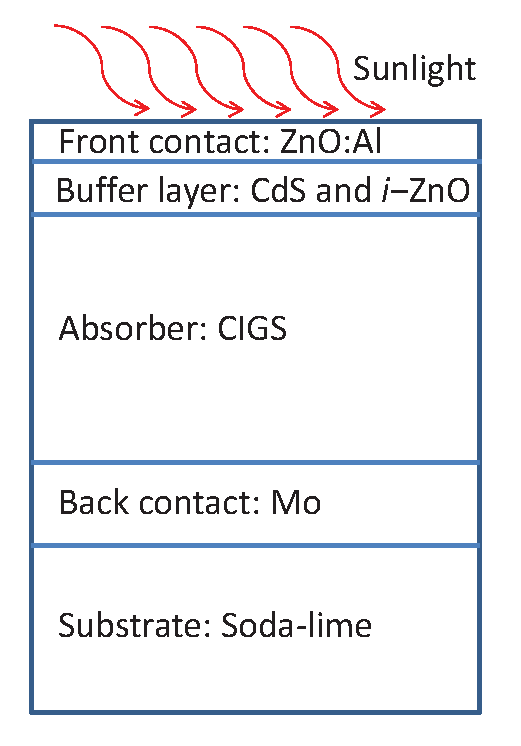
\includegraphics[scale=0.5]{cigsdevice.eps} 
\caption{Structure of CIGS solar cell device.}
\label{device}
\end{figure}

Substrate is on the bottom, and there are mainly three kinds of substrates: soda-lime glass, metal, and polyimide. The most common substrate is the one based on soda-lime glass containing sodium (Na) with thickness 
\SI{1} {\mm} to \SI{3} {\mm}. The Na can improve the efficiency and reliability of the solar cells as well as process tolerance. The molybdenum (Mo) works as a back contact due to its low resistivity and stability at high 
temperature with thickness around \SI{500} {\nm}. Most important part of the device is the $p$-type absorber layer: CIGS, which has intrinsic defects and its thickness is \SI{1500} - \SI{2000} {\nm}. 
The $n$-type buffer layer CdS is on the top of the CIGS, its thickness is around \SI{60} {\nm}. The intrinsic zinc oxide ($i$-ZnO) and $n$-type ZnO layers are followed, and they work as window layers. The $i$-ZnO is used to 
avoid damage of the CIGS and CdS from sputtering damage when depositing the ZnO:Al window layer. The $n$-type ZnO is doped by aluminum (Al) in order to get higher conductivity \cite{kim1997structural, minami1984highly}. 
This CIGS/CdS/ZnO structure is optimized to improve the cell performance. The detailed information about the structure CIGS solar cell device can be found in Refs.\cite{naghavi2010buffer,niki2010cigs, kessler2001baseline}.







\section{Theory}
\label{ch:dft}

\subsection{The quantum many-body problem}
\label{ch:mb}

\noindent A solid material contains a huge number of atoms (around 10\textsuperscript{23} \si{\per\cubic\centi\metre} ), and each atom consists of a nucleus surrounded by one or more electrons. 
According to the principles of quantum mechanics, all properties of a system are known if one can figure out a way to solve 
the quantum many-body Schrödinger equation. In this thesis, the time-independent many-body Schrödinger equation is only considered, which is given as

\begin{equation}\label{ssth}
 H^{en} {\Psi^{en}(\{ {\textbf r}_{i}, {\textbf R}_{I} \})} = {E^{en}} {\Psi^{en}(\{ {\textbf r}_{i}, {\textbf R}_{I} \})}.
\end{equation}


Here, superscript "$en$" implies that it is related with electrons and nuclei. ${\Psi^{en}(\{ {\textbf r}_{i}, {\textbf R}_{I} \})}$ is defined as many-particle wavefunction, $\textbf{r}_{i}$ 
and $\textbf{R}_{I}$ stands for coordinators of electron and nucleus. $E^{en}$ is defined as total energy of system. $H^{en}$ denotes Hamiltonian \cite{martin2004electronic}, which is defined in atomic units as

\begin{equation}\label{sth}\begin{split}
& H^{en} = - \sum\limits_i^{Ne}   \frac{{{\nabla}_{{i}}^{2}}}{2} - \sum\limits_I^{Nn} \frac{{{\nabla}_{{I}}^{2}}}{2 M_{I}}  - \sum\limits_i^{Ne} \sum\limits_I^{Nn} \frac{Z_{I}}{|\textbf{r}_{i}-\textbf{R}_{I}|} \\
& + \frac{1}{2} \sum\limits_i^{Ne} \sum\limits_{j \neq i}^{Ne} \frac{1}{ |\textbf{r}_{i}-\textbf{r}_{j}|} + \frac{1}{2} \sum\limits_I^{Nn} \sum\limits_{J \neq I}^{Nn} \frac{Z_{I} Z_{J}\ }{|\textbf{R}_{I}-\textbf{R}_{J}|}.
\end{split}\end{equation}

Here, indices $i$ and $j$ are used for the electrons, and $I$, $J$ are used for the atomic nuclei. $Z_I$ implies charge of the $I$:th nucleus.
$M_I$ denotes mass of the $I$:th nucleus in atomic units. The first and second terms are kinetic energy operator of the electrons and nuclei.
Other terms are Coulomb interactions between electrons and nuclei, electrons and electrons, and nuclei and nuclei in sequence.

\textbf{Eq. \ref{ssth}} can not be solved exactly. Moreover, the exact form of the wavefunction is unknown.
To approximate the exact solution, the process of finding the solution can be divided into three different levels generally \cite{martin2004electronic, Cottenierwien2k}: the first level is the Born-Oppenheimer approximation \cite{bornoppenheimer}; the second
level is Hartree approximation \cite{hartreeapproximation},
Hartree-Fock (HF) approximation \cite{hartreefockapproximation}, density functional theory (DFT) \cite{hohenberg1964inhomogeneous}, and Kohn-Sham (KS) equation \cite{kohn1965self}; the last level is to solve the secular 
equation, which is an equation solved to find eigenvalue of a matrix \cite{martin2004electronic, Cottenierwien2k}.

\subsection{The Born-Oppenheimer approximation}
\label{ch:boa}

\textbf{Eq. \ref{ssth}} should be approximated in order to solve it. A first step is to separate the wavefunction of electron and nucleus. The Schrödinger Hamiltonian in \textbf{Eq. \ref{sth}} has a coupling term between
the electron and nucleus, thereby one can not do that simply. Positions of nuclei can be treated as fixed because the mass of nucleus is much larger than that of electron. This indicates that the electrons are seen as interacting under
both the external potential caused by nuclei that are in fixed positions and that of the other electrons. The separation of motion between electrons and nuclei is called the Born-Oppenheimer approximation \cite{bornoppenheimer}.
Since the positions of nuclei are fixed, wavefunction can be written as

\begin{equation}\label{nwf}
{\Psi^{en}(\{ {\textbf r}_{i}, {\textbf R}_{I} \})} \   {\approx} \  {\theta(\{{\textbf R}_{I}\})} {\Psi(\{\textbf{r}_{i}\}; \{{\textbf R}_{I}\})}.
\end{equation}

Here, ${\Psi(\{\textbf{r}_{i}\}; \{{\textbf R}_{I}\})}$ denotes many-electron wavefunction in the Born-Oppenheimer approximation. Since the electrons are under the potential of nuclei, thus the wavefunction of 
electrons is related with the nucleus positions. 
 
\textbf{Eq. \ref{sth}} can be rewritten as

\begin{equation}\begin{split}\label{nh}
& {H^{en}} = H + H^n \\
& {H}\ = \ {U_e} \ + \ {U}_{ext} \ + \ {U}_{int}\  \\
& {H^n} = - \sum\limits_I^{Nn} \frac{{{\nabla}_{{I}}^{2}}}{2 M_{I}} + {{U}_{nn}}.
 \end{split}
\end{equation}

Furthermore, all the unknown terms in \textbf{Eq. \ref{nh}} are defined as

\begin{equation}\begin{split}\label{vext}
& {U_e} = - \sum\limits_i^{{Ne}}   \frac{{{\nabla}_{{i}}^{2}}}{2} \\
& U_{ext} = - \sum\limits_i^{{Ne}} \sum\limits_I^{{Nn}} \frac{Z_{I}}{|\textbf{r}_{i}-\textbf{R}_{I}|} \\
& {U}_{int} =  \frac{1}{2} \sum\limits_i^{{Ne}} \sum\limits_{j \neq i}^{{Ne}} \frac{1}{ |\textbf{r}_{i}-\textbf{r}_{j}|} \\
& {{U}_{nn}} = \frac{1}{2} \sum\limits_I^{{Nn}} \sum\limits_{J \neq I}^{{Nn}} \frac{Z_{I} Z_{J}\ }{|\textbf{R}_{I}-\textbf{R}_{J}|}.
\end{split}
\end{equation}

Here, $H$ represents Hamiltonian for the many-electron system within the Born-Oppenheimer approximation. The subscript $ext$ implies $external$ in \textbf{Eq. \ref{nh}}, thus $U_{ext}$ describes
the external potentials interaction $V_{ext}({\textbf{r}})$. 

The new Schrödinger equation combined with \textbf{Eq. \ref{nwf}} and \textbf{Eq. \ref{nh}} is given as

\begin{equation}\label{chenadd1}
 \Big( H+ {H}^n \Big) \Big({\theta(\{{\textbf R}_{I}\})} {\Psi(\{\textbf{r}_{i}\}; \{{\textbf R}_{I}\})} \Big) =
 E^{en}(\{{\textbf R_I}\}) \Big({\theta(\{{\textbf R}_{I}\})} {\Psi(\{\textbf{r}_{i}\}; \{{\textbf R}_{I}\})}\Big).
\end{equation}
 
\noindent Here, $E^{en}(\{{\textbf R }_I\})$ represents system total energy, which is ${\textbf R}_I$-dependent because system wavefunction depends on nuclei positions. 
One ends up with the following equation taking \textbf{Eq. \ref{vext}} and \textbf{Eq. \ref{chenadd1}}.

\begin{equation}\begin{split}\label{ise}
& {H} {\Psi(\{\textbf{r}_{ i}\}; \{{\textbf R}_{ I}\})} = E{(\{\textbf{R}_{ I}\})} {\Psi(\{\textbf{r}_{i}\}; \{{\textbf R}_{I}\})} \\
& \Big( {U}_{nn1}+{U}_{nn2}+{U}_{nn3}+{U}_{nn}+E(\{{\textbf R}_{I}\}) \Big) {\theta(\{\textbf{R}_{I}\})} = E^{en}(\{{\textbf R}_I\}) {\theta(\{\textbf{R}_{I}\})}.
\end{split}
\end{equation}

\noindent Here, $E{(\{\textbf{R}_{I}\})}$ denotes the total energy of many-electron system, which is also ${\textbf R}_I$-dependent because electrons wavefunction indirectly depends on nuclei positions. The ${U}_{nn1}$,
${U}_{nn2}$, and ${U}_{nn3}$ in \textbf{Eq. \ref{ise}} are derived as

\begin{equation}\begin{split}
 &  {U}_{nn1} = - \sum\limits_I^{{Nn}} \frac{{{\nabla}_{{I}}^{2}}}{2 M_{I}}   \\
 &  {U}_{nn2} = - \sum\limits_I^{{Nn}} \frac{1}{M_{I}} {\int {\Psi(\{\textbf{r}_{{i}}\}; \{\textbf{R}_{I}\})}^{\ast} {{\nabla}_{{I}}} {{\Psi(\{\textbf{r}_{{i}} \}; \{\textbf{R}_{I}\})}} d {\textbf r }} {{\nabla}_{{I}}}  \\
 &  {U}_{nn3} = - \sum\limits_I^{{Nn}} \frac{1}{M_{I}} {\int {{\Psi(\{\textbf{r}_{{i}}\}; \{\textbf{R}_{I}\})}}^{\ast} {{\nabla}_{{I}}^{2}} {{\Psi(\{\textbf{r}_{{i}} \}; \{\textbf{R}_{I}\})}} d {\textbf r }}. 
\end{split}\end{equation}

In \textbf{Eq. \ref{ise}}, one observes that the lattice dynamical properties of certain system within the Born-Oppenheimer approximation can be obtained. To solve this equation,
the ground state energy $E(\{{{\textbf R}_{I}}\})$ of many-electron system is needed. Here, $\{{\textbf R}_{I}\}$ denotes a sef of atom positions.
 
In summary, the Schrödinger equations of electrons and nuclei are derived separately within the Born-Oppenheimer approximation. When one calculates ground state properties,
the Schrödinger equation of the electrons is applied (the first line in \textbf{Eq. \ref{ise}}). The Schrödinger equation of nuclei is employed for the calculations of lattice dynamics 
($U_{nn2}$ and $U_{nn3}$ are ignored \cite{clasdft} in the second line in \textbf{Eq. \ref{ise}} normally).

The \textbf{Eq. \ref{ise}} (the first line) is much simpler than \textbf{Eq. \ref{ssth}}. However, it is still not solvable. Further approximations  are needed
to solve this many-body problem.

\subsection{Solving the many-body problem}

In previous section, the separation of wavefunction is proposed within Born-Oppenheimer approximation. The quantum many-body Schrödinger problem becomes the many-electron 
Schrödinger problem. There are two major problems from the Born-Oppenheimer approximation: the first problem is that the number of electron is around in the order of 10\textsuperscript{24} \si{\per\cubic\centi\metre} in most
of the cases, which is a huge numerical problem. However, it is still possible to solve; the second one is that the Hamiltonian includes operators acting on the single electron. However, how the relation between the wavefunction and
the single-electron wavefunction is unknown. The latter problem can be solved by one of the following three methods: the first method is to figure out a way to separate or approximate the wavefunction from the single-electron function,
such as the Hartree and Hartree-Fock (HF) methods \cite{hartreeapproximation,hartreefockapproximation}; the second method is to find an explicit relation between total energy and wavefunction, such as density functional theory (DFT)
\cite{hohenberg1964inhomogeneous}. Within DFT, the system total energy is a functional of electron density. Either of these two methods has "pros and cons"; the third one is called Kohn-Sham
equation \cite{kohn1965self}, which is a combination of above two methods. It starts from DFT, and takes advantage of single-electron wavefunction.

\subsubsection{Hartree approximation}
\label{ha}
The simplest approximation of wavefunction for many-electron Schrödinger equation is the one acting like independent
electrons. The wavefunction with $Ne$ independent electrons is defined as

\begin{equation}\label{wfh}
\wfh = \bwff<1><1> \bwff<2><2> \cdots \bwff<Ne><Ne>. 
\end{equation}

Here, $\bwff<i><i>$ implies state of the $i$:th electron, where different states of electrons are orthonormalized. From here on, the $\{{\textbf R}_I\}$ are suppressed in the
wavefunction since atoms are treated as in fixed positions. The set of variables ${\{\textbf{r}_{{i}}}\}$ includes the coordinates of space and spin. The total energy of the many-electron system can be written as

\begin{equation}\label{teh}
E^{{H}} = <\wfh |\ {\hath} \ | \wfh  >.
\end{equation}

${\hath}$ in \textbf{Eq. \ref{nh}} can be rewritten as
\begin{equation}\begin{split}
&  {\hath} = \sum\limits_i^{{Ne}} \Big( -\frac{{{\nabla}_{{i}}^{2}}}{2} - \sum\limits_I^{{Nn}} \frac{Z_{I}}{|\textbf{r}_{i}-\textbf{R}_{I}|} \Big) +   \frac{1}{2} \sum\limits_i^{{Ne}} \sum\limits_{j \neq i}^{{Ne}} \frac{1}{ |\textbf{r}_{i}-\textbf{r}_{j}|} \\
& = \sum\limits_i^{{Ne}} h_1(\textbf{r}_{i}) + \frac{1}{2} \sum\limits_i^{{Ne}} \sum\limits_{j \neq i}^{{Ne}} h_2(\textbf{r}_{i},\textbf{r}_{j}).
\end{split}
\end{equation}

Therefore, the system total energy is given as
\begin{equation}\begin{split}\label{bzd}
& E^{H} = \sum\limits_i^{{Ne}} <\bwff<i><i> | \  h_1(\textbf{r}_{i}) \ | \bwff<i><i> > \\
& +\frac{1}{2} \sum\limits_i^{{Ne}} \sum\limits_{j \neq i}^{{Ne}} <\bwff<i><i> \bwff<j><j>|\ h_2(\textbf{r}_{i},\textbf{r}_{j}) \ | \bwff<i><i> \bwff<j><j>>.  
\end{split}\end{equation}

In order to calculate the stationary state with the lowest energy of the system, one method called Lagrange multipliers can be utilized. Furthermore, the constraint is that the different states of electrons are orthonormalized.
Therefore, the variation with respect to any wavefunction $\phi^*_{k}(\textbf{r})$ and Lagrange multiplier $E_{i,j}^{H}$ are satisfied \cite{clasdft,bertsekas2003convex}

\begin{equation}\begin{split}\label{haa}
 \frac{ \delta  \Big(E^{{H}} - \sum\limits_{i}^{Ne} \sum\limits_{j}^{Ne} E_{i,j}^{H} (<\bwff<i><i> | \bwff<j><j>> -\ \delta_{ij})\Big)}{\delta \phi^*_{k}(\textbf{r})}  = 0. 
\end{split}
\end{equation}


Here, $ \delta \phi_{k}(\textbf{r})$ also can be utilized. However, variation with respect to $\phi^*_{k}(\textbf{r})$ and $\phi_{k}(\textbf{r})$ are equivalent. It is convenient to use $\delta \phi^*_{k}(\textbf{r})$.

$\delta E^{{H}}$ in \textbf{Eq. \ref{haa}} can be calculated by two parts. The first part is 

\begin{equation}\begin{split}\label{hartree1}
&  \delta ( \sum\limits_i^{{Ne}} <\bwff<i><i> |\ h_1(\textbf{r}_{i})  \ | \bwff<i><i> > )  \\
& =  < \delta \phi_{{k}}(\textbf{r}) |\ h_1(\textbf{r})  \ |  \phi_{{k}}(\textbf{r}) >  +  < \phi_{{k}}(\textbf{r}) |\ h_1(\textbf{r})  \ | \delta \phi_{{k}}(\textbf{r}) >. 
\end{split}\end{equation}

The second part is

\begin{equation}\begin{split}\label{hartree2}
& \frac{1}{2} \delta \sum\limits_i^{{Ne}} \sum\limits_{j \neq i}^{{Ne}} <\bwff<i><i> \bwff<j><j>|\ h_2(\textbf{r}_{i},\textbf{r}_{j}) \ | \bwff<i><i> \bwff<j><j>> \\
& = \frac{1}{2}  \sum\limits_{i \neq k}^{{Ne}} \Big( <\bwff<i><i>  \delta \bwff<k><>|\ h_2(\textbf{r}_{i},\textbf{r}) \ | \bwff<i><i> \bwff<k><>> \\
& + <\bwff<i><i>  \bwff<k><>|\ h_2(\textbf{r}_{i},\textbf{r}) \ | \bwff<i><i> \delta \bwff<k><>> \Big) \\
& + \frac{1}{2}  \sum\limits_{j \neq k}^{{Ne}} \Big( <\delta \bwff<k><>  \delta \bwff<j><j>|\ h_2(\textbf{r},\textbf{r}_{j}) \ | \bwff<k><> \bwff<j><j>> \\
& + < \bwff<k><>  \bwff<j><j>|\ h_2(\textbf{r},\textbf{r}_{j}) \ | \delta \bwff<k><> \bwff<j><j>> \Big) \\
& =   \sum\limits_{i \neq k}^{{Ne}} \Big( <\bwff<i><i>  \delta \bwff<k><>|\ h_2(\textbf{r}_{i},\textbf{r}) \ | \bwff<i><i> \bwff<k><>> \\
& + <\bwff<i><i>  \bwff<k><>|\ h_2(\textbf{r}_{i},\textbf{r}) \ | \bwff<i><i> \delta \bwff<k><>> \Big). 
\end{split}\end{equation}

Here, the factor of $\frac{1}{2}$ is cancelled because the $2$nd ($3$rd) line is the same with $4$th ($5$th) line in \textbf{Eq. \ref{hartree2}} due to the exchangeable indices of $i$ and $j$. 

To get the final solution, one more calculation is needed 

\begin{equation} \begin{split}\label{xixihaha}
& \delta \sum\limits_i^{{Ne}} \sum\limits_j^{{Ne}} E_{i,j}^{{H}} \Big(<\phi_{i}(\textbf{r}_{i}) | \phi_{j}(\textbf{r}_{j}) > - \ \delta_{i,j}\Big) \\
& = \sum\limits_j^{{Ne}} E_{k,j}^{{H}} \Big(< \delta \phi_{k}(\textbf{r}) | \phi_{j}(\textbf{r}_{j}) > \Big) + \sum\limits_i^{{Ne}} E_{i,k}^{{H}} \Big(<\phi_{i}(\textbf{r}_{i}) | \delta \phi_{k}(\textbf{r}) >\Big) \\
& = \sum\limits_i^{{Ne}} E_{k,i}^{{H}} \Big(< \delta \phi_{k}(\textbf{r}) | \phi_{i}(\textbf{r}_{i}) >  + <\phi_{i}(\textbf{r}_{i}) | \delta \phi_{k}(\textbf{r}) >\Big).
\end{split}
\end{equation}


Therefore, \textbf{Eq. \ref{haa}} can be derived as 

\begin{equation}\label{hartreq11}
\Big(-\frac{\nabla^{2}_{k}}{2} + \sum\limits_I^{{Nn}} \frac{Z_{I}}{|\textbf{r}-\textbf{R}_{I}|} + \sum\limits_{j \neq k}^{{Ne}}  <\bwfn<j><'>\ | \frac{1}{|\textbf{r} - \textbf{r}^{'} |} \ | \bwfn<j><'>>\Big) \bwff<k><> = \sum\limits_i^{{Ne}} E_{k,i}^{H} \bwff<i><>.
\end{equation}

There are many solutions in \textbf{Eq. \ref{hartreq11}}, and each corresponds to a different set of $E_{k,i}^{H}$. One can choose to the $E_{k,i}^{H}$, which satisfies $E_{k,i}^{H}$ = $\delta_{k,i}\epsilon_k^{{H}}$.
\textbf{Eq. \ref{hartreq11}} can be rewritten as

\begin{equation}\begin{split}\label{hartreq}
& \Big(-\frac{\nabla^{2}_{k}}{2} + \sum\limits_I^{{Nn}} \frac{Z_{I}}{|\textbf{r}-\textbf{R}_{I}|} + \sum\limits_{j \neq k}^{{Ne}}  <\bwfn<j><'>\ | \frac{1}{|\textbf{r} - \textbf{r}^{'} |} \ | \bwfn<j><'>>\Big) \bwff<k><> = \epsilon_k^{{H}} \bwff<k><>  \\
&  \qquad \qquad \qquad  \qquad \qquad \qquad \qquad \qquad  \Downarrow  \\
& \Big(-\frac{\nabla^{2}_{i}}{2} + \sum\limits_I^{{Nn}} \frac{Z_{I}}{|\textbf{r}-\textbf{R}_{I}|} + \sum\limits_{j \neq i}^{{Ne}}  <\bwfn<j><'>\ | \frac{1}{|\textbf{r} - \textbf{r}^{'} |} \ | \bwfn<j><'>>\Big) \bwff<i><> = \epsilon_i^{{H}} \bwff<i><>.  \\
\end{split}
\end{equation}


Here, \textbf{Eq. \ref{hartreq}} is a group of dependent single particle equations. $\epsilon_k^{{H}}$ is identified as the eigenvalue for this single-electron Hartree equation.

\subsubsection{Hartree-Fock approximation}
Hartree approximation is a simple approximation. Hartree-Fock (HF) approximation is a method which considers antisymmetry of wavefunction. It is shown as

\begin{equation}\label{hfwf}
\Psi^{HF} ( \cdots \textbf{r}_{i} \cdots  \textbf{r}_{j} \cdots ) = - \Psi^{HF} ( \cdots \textbf{r}_{j} \cdots  \textbf{r}_{i} \cdots).
\end{equation}

Here, each variable ${\textbf{r}_{{i}}}$ includes the coordinates of space and spin. Slater introduced a way to construct the wavefunction subject to \textbf{Eq. \ref{hfwf}} \cite{slater1951simplification}. The wavefunction of the many-electron 
Schrödinger equation is described in a matrix determinant for the $N$ number of electrons (for aesthetic reason, $N$ implies the number of electrons and not $Ne$ as in previous sections)

\begin{equation}\label{hfwfm}
\Psi^{HF}(\textbf{r}_1, \textbf{r}_2, \ldots, \textbf{r}_N) =
\frac{1}{\sqrt{N!}} \left|
\begin{matrix}
    \bwff<1><1> & \bwff<2><1> & \cdots & \bwff<N><1> \\
    \bwff<1><2> & \bwff<2><2> & \cdots & \bwff<N><2> \\
    \vdots               & \vdots               &        & \vdots               \\
    \bwff<1><N> & \bwff<2><N> & \cdots & \bwff<N><N>
\end{matrix} \right|.
\end{equation}
\noindent Here, the factor in front ensures normalization, and $\bwff<i><i>$ implies state of the ($i$):th electron. \textbf{Eq. \ref{hfwfm}} has the antisymmetry property of wavefunction.

The total energy of Hartree-Fock approximation, which can be determined similarly as in the previous section of Hartree approximation, is given as

\begin{equation}\begin{split}
&E^{HF} = \sum\limits_i^{{N}} <\bwff<i><> |\ -\frac{\nabla^{2}_{i}}{2} + \sum\limits_I^{{Nn}} \frac{Z_{I}}{|\textbf{r}-\textbf{R}_{I}|}  \ | \bwff<i><> > \\
& + \frac{1}{2} \sum\limits_i^{{N}} \sum\limits_j^{{N}} <\bwff<i><> \bwfn<j><'>|\ \frac{1}{|\textbf{r} - \textbf{r}^{'} |} \ | \bwff<i><> \bwfn<j><'>> \\
& - \frac{1}{2} \sum\limits_i^{{N}} \sum\limits_j^{{N}} <\bwfn<i><'> \bwfn<j><>|\ \frac{1}{|\textbf{r} - \textbf{r}^{'} |} \ | \bwfn<i><> \bwfn<j><'>>.
\end{split}\end{equation}

Here, there is no contribution to the sum when $i$ = $j$. In the same mathematical way as in previous section but somewhat more complicated, the single particle Hartree-Fock equation can be obtained

\begin{equation}\begin{split}\label{above1}
& \Big( -\frac{\nabla^{2}_{i}}{2} + \sum\limits_I^{{Nn}} \frac{Z_{I}}{|\textbf{r}-\textbf{R}_{I}|} + \sum\limits_{j}^{{N}} <\bwfn<j><'>\ | \frac{1}{|\textbf{r} - \textbf{r}^{'} |} \ | \bwfn<j><'>> \Big) \bwff<i><>  \\
& - \sum\limits_{j}^{{N}}  < \bwfn<j><'>|\ \frac{1}{|\textbf{r} - \textbf{r}^{'} |} \ | \bwfn<i><'> > \bwfn<j><>  = \epsilon_{i}^{{HF}} \bwff<i><>.
\end{split}\end{equation}

In comparison with Hartree equation in \textbf{Eq. \ref{hartreq}}, there is an extra term in \textbf{Eq. \ref{above1}}, which is so called exchange term. In order to show the equation in a more well organized way,
\textbf{Eq. \ref{above1}} is equivalent to

\begin{equation}\label{aaaaa}\begin{split}
& \Big( -\frac{\nabla^{2}_{i}}{2} +  \sum\limits_I^{{Nn}} \frac{Z_{I}}{|\textbf{r}-\textbf{R}_{I}|} +V_{HF}(\textbf{r}) \Big)  \bwff<i><>  = \epsilon_{i}^{{HF}}   \bwff<i><> \\
&  V^{HF}(\textbf{r})= \int \frac{\rho(\textbf{r}{'}) - \rho_{{i}}^{{HF}}(\textbf{r},\textbf{r}{'})}{|\textbf{r} - \textbf{r}{'} |}  \mathrm{d}\textbf{r}{'} \\
& \rho_{{i}}^{{HF}}(\textbf{r},\textbf{r}{'}) = \sum\limits_j^N \frac{\phi_{i}^{}(\textbf{r}{'}) \phi_{i}^{*}(\textbf{r}{}) \phi_{j}^{}(\textbf{r}{}) \phi_{j}^{*}(\textbf{r}{'})} {\phi_{i}^{}(\textbf{r}) \phi_{i}^{*}(\textbf{r})}  \\
& \rho(\textbf{r}) = \sum\limits_i^N  {|\bwff<i><>|}^{2}.
\end{split}
\end{equation}


\subsubsection{Density functional theory}
The Hartree and HF methods are very classic methods solving the many-electron Schrödinger equation. However, the HF method only includes the exchange term and not the electron correlation term. Therefore, it is not suitable 
for solid materials. Apart from the Hartree and HF methods, there is a modern method solving the more complicated calculations of many-electron system, namely density functional theory (DFT). 
It is introduced by Hohenberg and Kohn in 1964 \cite{hohenberg1964inhomogeneous}. Kohn and Pople were awarded Chemistry Nobel Prize in 1998.

The idea of the DFT is to treat the electron density in solid materials instead of using the many-particle wavefunction. In this case, the degree of freedom reduces from 3$N$ ($N$ is the number of electrons) to 3.
It is apparently less complicated than Hartree and HF methods. 

$\textbf{The density as basic variable}$ 

There are two questions coming out if considering the electron density as a role of wavefunction. The first one is whether it is the equivalence relation between electron density and wavefunction in many-electron system. 
The second one is how to solve the problem if considering the electron density instead of the wavefunction. In order to explain above two questions, there are two very basic theorems introduced by Hohenberg and Kohn:

\begin{thm}
\label{hk1}
\noindent The first theorem states that the external potential $V_{ext}(\textbf{r})$  is determined uniquely for any many-electron system by the ground-state electron density $\rho$.
\end{thm}

The above theorem indicates that all ground state properties are determined by the true ground-state density $\rho$ as well,
such as, the total energy $E$ = $E$[$\rho$]. 

The above theorem also explains the equivalence relation between the electron density and wavefunction. Hamiltonian is obtained from external potential,
thus the wavefunction is obtained from the external potential. Therefore, the corresponding electron density is determined. Moreover, the external potential is unique decided by electron
density from the theorem. Therefore, the electron density contains the same information as the wavefunction.

Proof of the theorem is given. Let us assume that there exists two external potentials named $V_{ext}(\textbf{r})$ and $V'_{ext}(\textbf{r})$ leading to the same ground state 
electron density $\rho$. Obviously, this will lead to two different Hamiltonians, that is, ${H}$ and ${H'}$, as well as two different corresponding
wavefunctions named $\Psi$ and $\Psi'$. Since $\Psi$ is not the ground state wavefunction of ${H'}$, the same rules to $\Psi'$ and ${H}$, two following
inequality equations are satisfied

\begin{equation}\label{hkpf1}\begin{split}
&  E = \langle \Psi\ |{H}|\ \Psi \rangle  \ < \  \langle \Psi'\ |{H}|\ \Psi' \rangle \\
&  E' = \langle \Psi'\ |{H'}|\ \Psi' \rangle  \ < \  \langle \Psi\ |{H'}|\ \Psi \rangle.
\end{split}\end{equation}

Taking advantage of the Hamiltonian from \textbf{Eq. \ref{nh}}, the following equation is derived
\begin{equation}\label{hkpf2}\begin{split}
&    \langle \Psi'\ |{H}|\ \Psi' \rangle \\
&  = \langle \Psi'\ |{H'} + {H} - {H'}|\ \Psi' \rangle \\
&  = \langle \Psi'\ |{H'} |\Psi' \rangle + \langle \Psi' | {H} - {H'}|\ \Psi' \rangle \\
&  = E' + \int \Big( V_{ext}(\textbf{r}) - V'_{ext}(\textbf{r}) \Big)  \rho(\textbf{r}) d \textbf{r}.
\end{split}\end{equation}

Using \textbf{Eq. \ref{hkpf1}} and \textbf{Eq. \ref{hkpf2}}, the following relation is given by

\begin{equation}\label{hkpf3}
 E  < \  E' + \int \Big( V_{ext}(\textbf{r}) - V'_{ext}(\textbf{r}) \Big)  \rho(\textbf{r}) d \textbf{r} .
\end{equation}

Another similar inequality equation can be obtained if one changes the equation $\langle \Psi\ |{H'}|\ \Psi \rangle$ like \textbf{Eq. \ref{hkpf2}}
\begin{equation}\label{hkpf44}
  E'  < \  E + \int \Big( V'_{ext}(\textbf{r}) - V_{ext}(\textbf{r}) \Big)  \rho(\textbf{r}) d \textbf{r} .
\end{equation}

Plus the left side and right side from both \textbf{Eq. \ref{hkpf3}} and \textbf{Eq. \ref{hkpf44}}, a contradictory result is given as
\begin{equation}\label{hkpf4}
  E + E'  < \  E' + E.
\end{equation}

Since this is an incorrect relation, the external potential $V_{ext}(\textbf{r})$ has to be unique.

\begin{thm}
\label{hk2}
\noindent The second theorem states that there is a universal functional $F[\rho]$ for the total energy in the terms of the electron density $\rho$ with any external potential $V_{ext}(\textbf{r})$ ,
and the exact ground-state density is obtained when the ground state total energy functional reaches its minimal value, that is, E[$\rho'$]>E[$\rho$]. Here, $\rho$ is the exact ground-state density.
\end{thm}

Proof of theorem is given. Because of the first theorem, the kinetic and interaction energies are functional of electron density. The total energy can be expressed in the following way (ignoring the interaction between nuclei)
\begin{equation}\label{hkpf5}\begin{split}
& E[\rho] \ = \langle \Psi  | \ {U_e} \ + \ {U}_{int}  \ + \ {U}_{ext} \ | \Psi \rangle \\
&     = \langle \Psi  | \ {V}_{ext}(\textbf{r}) \ | \Psi \rangle  + \underbrace{\langle \Psi  | \ {U_e} \ + \ {U}_{int}  \ \ | \Psi \rangle}  \\
&     =   \ \int \rho(\textbf{r}) V_{ext}(\textbf{r}) \mathrm{d}\textbf{r} \quad +  \quad F[\rho]. 
\end{split}
\end{equation}

In \textbf{Eq. \ref{hkpf5}}, the term of $F[\rho]$ is a universal functional for all the many-electron system.

The functional of total energy $E[\rho']$ reaches the minimum at the exact ground-state electron density $\rho$
\begin{equation}\begin{split}
 & E[\rho'] \ =   \ \int \rho'(\textbf{r}) V_{ext}(\textbf{r}) d \textbf{r}   + \  F[\rho'] > E[\rho]. 
\end{split}
\end{equation}
 
Here, the total energy for the case of exact ground-state electron density is lower than any other cases. Therefore, the exact ground-state electron density by minimizing the total energy can be achieved.

From those two theorems, one knows how to solve Schrödinger equation theoretically. However, $E[\rho]$ is unknown in practice. Therefore, another method is needed to solve this problem, which is so called Kohn-Sham (KS) equation.

\subsubsection{Kohn-Sham equation}

The Hartree and HF methods are introduced to solve the many-body problem, both of which are based on the idea of transforming complex 
many-electron problem to single-electron problem by using different wavefunctions. The DFT gives the answer to solve many-electron system, however, it does not give explicit expression.
This problem in DFT is solved by KS equation, which was introduced by Kohn and Sham in 1965 \cite{kohn1965self}. It is demonstrated in the following text (ignoring the interaction between nuclei).

Assume that the exact ground-state density is obtained by the Hartree-like wavefunction $\wfks = \bwf<1><1> \bwf<2><2> \cdots \bwf<N><N>$. Here, $N$ is the number of electrons, and $\bwf<i><i>$ is an auxiliary independent
single-electron wavefunction. The electron density is defined as

\begin{equation}\label{ks1}
 \rho(\textbf{r}) = \sum\limits_i^{N} {\Psi^{{KS}*}_{i}(\textbf{r})} {\Psi^{{KS}}_{i}(\textbf{r})}.
\end{equation}

If the electron density is exact, thus the total energy is exact. It is given as

\begin{equation}\label{kse}
\begin{split}
&E[\rho] \ =\ T[\rho] \ + \ V_{int}[\rho] \ + \ V_{ext}[\rho]  \\
&\ \ \   = \ T_{0}[\rho] \ + \ V_{H}[\rho] \ + V_{ext}[\rho]+\underbrace{\ (T[\rho] \ - \ T_{0}[\rho]) \ + \  (V_{int}[\rho] \ - \ V_{H}[\rho])\ }       \\
&\ \ \   = \ T_{0}[\rho] \quad \,  + \quad \,  V_{H}[\rho] \quad \, + \quad \, V_{ext}[\rho] \quad \, + \quad \, E_{xc}[\rho].
\end{split}
\end{equation}

Here, $E[\rho]$ denotes total energy, and $\rho$ denotes ground-state density. $T[\rho]$, $V_{int}[\rho]$, and $V_{ext}[\rho]$ represent energies from the exact kinetic, 
the exact electron-electron potential, and external potential in sequence. $E_{xc}[\rho]$ is unknown exchange-correlation energy.

The $T_{0}[\rho]$, $V_{H}[\rho]$, and $V_{ext}[\rho]$ represent kinetic energy in the Hartree approximation, electron interaction energy in Hartree approximation, and electron-nuclei interaction energy in sequence.

\begin{equation}\begin{split}\label{kankan}
& T_{0}[\rho]\ = \sum\limits_i^{N} \ < \Psi_{i}^{{KS}}(\textbf{r}) \ | -\frac{\nabla^{2}}{2} \ | \Psi_{i}^{{KS}}(\textbf{r}) > \\
& V_{H}[\rho] \ = \ \frac{1}{2} \int \int  \frac{\rho({\textbf{r}})\rho(\textbf{r}')}{|{\textbf{r}}-{\textbf{r}}'|} \mathrm{d} {\textbf{r}} \mathrm{d}{\textbf{r}'}\\
& V_{ext}[\rho]\ = \ \int  \rho(\textbf{r}) V_{ext}(\textbf{r})\mathrm{d}{\textbf{r}}. 
\end{split}
\end{equation}

In order to derive the ground state properties in the many-electron system, one can view this problem as the process of minimizing the total energy by varying the wavefunction $\Psi^{{KS}*}_{{k}}(\textbf{r})$. 

\begin{equation}\begin{split}\label{ks11}
& \frac{ \delta  \Big(E[\rho] - \sum\limits_{i}^{Ne} \sum\limits_{j}^{Ne} E_{i,j}^{H} (<\Psi^{{KS}}_{{i}}(\textbf{r}_i) | \Psi^{{KS}}_{{j}}(\textbf{r}_j)> -\ \delta_{ij})\Big)}{\delta \Psi^{{KS}*}_{{k}}(\textbf{r})}  = 0 \\
&  \qquad \qquad \qquad  \qquad \qquad \qquad  \Downarrow \\
& \frac{\delta T_{0}[\rho]}{\Psi^{{KS}*}_{{k}}(\textbf{r})} + \frac{\delta(V_{H}[\rho]  + V_{ext}[\rho] + E_{xc}[\rho])}{\delta \rho(\textbf{r})} \frac{\delta \rho(\textbf{r})}{\Psi^{{KS}*}_{{k}}(\textbf{r})} 
= \sum\limits_i^{{N}} E_{k,i}^{KS} \Psi^{{KS}}_{{i}}(\textbf{r}).
\end{split}
\end{equation}


The derivation is similar as in the section of Hartree approximation, the KS equation is derived as 

\begin{equation}\label{aaa}
 \Big(-\frac{\nabla^{2}}{2}\ + \ V^{KS}(\textbf{r})\Big) \Psi^{{KS}}_{{i}}(\textbf{r}) = \epsilon^{{KS}}_{{i}} \Psi^{{KS}}_{{i}}(\textbf{r}).
\end{equation}

Here, $\epsilon^{{KS}}_{{i}}$ is identified as eigenvalue for the KS equation. The $V^{KS}(\textbf{r})$ is give as

\begin{equation}\begin{split}\label{xiahunao}
&\ V^{KS}(\textbf{r}) \ = \ V_{ext}(\textbf{r}) + \int \mathrm{d}{\textbf{r}'}  \frac{\rho(\textbf{r}')}{|{\textbf{r}}-{\textbf{r}}'|} \ + \ \frac{\delta{E_{xc}}}{\delta{\rho(\textbf{r})}} \\
&\ = \ \ V_{ext}(\textbf{r}) + \int \mathrm{d}{\textbf{r}'}  \frac{\rho(\textbf{r}')}{|{\textbf{r}}-{\textbf{r}}'|} \ + \ V_{xc}(\textbf{r}).
\end{split}
\end{equation}

In \textbf{k}-space, KS equation in \textbf{Eq. \ref{aaa}} can be written as
\begin{equation}\label{aaa111}
 \Big(-\frac{\nabla^{2}}{2}\ + \ V^{KS}(\textbf{r})\Big) \Psi^{{KS}}_{{i,k}}(\textbf{r}) = \epsilon^{{KS}}_{{i,k}} \Psi^{{KS}}_{{i,k}}(\textbf{r}).
\end{equation}


The total energy is not given in \textbf{Eq. \ref{aaa}}. However, if one changes \textbf{Eq. \ref{aaa}} as 
\begin{equation}\label{bbb}
\sum\limits_i^N \Psi^{{KS}*}_{{i}}(\textbf{r}) \Big(-\frac{\nabla^{2}}{2}\ + \ V^{KS}(\textbf{r})\Big) \Psi^{{KS}}_{{i}}(\textbf{r}) = \sum\limits_i^N \Psi^{{KS}*}_{{i}}(\textbf{r}) \epsilon^{{KS}}_{{i}}  \Psi^{{KS}}_{{i}}(\textbf{r}).
\end{equation}

Based on \textbf{Eq. \ref{kankan}} , \textbf{Eq. \ref{kse}}, and \textbf{Eq. \ref{bbb}}, the total energy expression is derived as
\begin{equation}\label{totalenergy}
\begin{split}
& E[\rho] = \sum\limits_i^N \epsilon^{{KS}}_{{i}} - \ \frac{1}{2} \int \int \mathrm{d} {\textbf{r}} \mathrm{d}{\textbf{r}'} \frac{\rho({\textbf{r}})\rho(\textbf{r}')}{|{\textbf{r}}-{\textbf{r}}'|} \\
&    + \ E_{xc}[\rho] - \int   V_{xc}(\textbf{r}) \rho({\textbf{r}}) \mathrm{d} {\textbf{r}}.
\end{split}
\end{equation}

There are two problems still in the air: one is the exact format of $V_{xc}(\textbf{r})$; the other one is how to solve the KS equation.

\subsubsection{The exchange-correlation potential}

The exchange-correlation potential is the most difficult part during the process of solving the KS equation, because the exact form is still unknown today. Therefore, there
 are varies of approximations about it, such as the local density approximation (LDA) \cite{martin2004electronic, Cottenierwien2k, kohn1965self, von1972local, hedin1971explicit}.

$\textbf{The local density approximation}$

The LDA is a simple way to approximate the exchange-correlation part. It is based on free electron gas, which has a constant electron density 

\begin{equation}
 \rho(\textbf{r}) = \rho = \frac{N}{V}.
\end{equation}

Here, $N$ is number of electrons within solid, and $V$ is volume of solid. The exact exchange-correlation energy per electron is given as

\begin{equation} 
 \varepsilon_{xc}^{gas}(\rho) = -\frac{3}{4}\cdot(\frac{3}{\pi})^{1/3}\cdot{\rho}^{1/3} + 
 \begin{cases} A\ln{r_s}+B+C{r_s}\ln{r_s}+D{r_s} & \quad \mbox{if ${r_s} \leq 1 $} 
\\
 \gamma / (1+\beta_1 \sqrt{{r_s}}+ \beta_2 {r_s}) & \quad \mbox{if ${r_s} > 1$ }.\\ 
\end{cases} 
\end{equation}

Here, $r_s = (3 / (4 \pi \rho))^{1/3}$. In the LDA, the idea is that the exchange-correlation energy for an electron in a very tiny small volume in many-particle system is equal to the exchange-correlation for an electron 
in the free electron gas with the same density in the volume ($\varepsilon_{xc}^{gas}(\rho(\textbf{r}))$ = $\varepsilon_{xc}^{gas}(\textbf{r})$). The explicit exchange-correlation energy is given as

\begin{equation}
 E^{LDA}_{xc}[\rho] = \int \rho(\textbf{r}) \varepsilon_{xc}^{gas}( \textbf{r} ) \mathrm{d} \textbf{r}.
\end{equation}

Therefore, the exchange-correlation potential is give as
\begin{equation}
 V_{xc}^{LDA}(\textbf{r}) = \frac{\delta  E^{LDA}_{xc}[\rho]}{\delta \rho}.
\end{equation}

Today, there exists hundreds of different exchange-correlation potentials \cite{tozer1998development, hamprecht1998development, grabo1995density, cohen2007development}. It is still ongoing development.
The advantage of KS equation is that new potentials are implemented easily. In the same time, it has many potentials due to
the simplicity of implementation.

\subsection{Solving the secular equation}

The process for solving KS equation can be achieved by iteration \cite{martin2004electronic, Cottenierwien2k, clasdft}. Potential in KS equation depends on electron density.
However, electron density is calculated by wavefunction, which depends on the potential. 
An initial guess of electron density is calculated at the beginning of calculation, then the KS equation is solved iteratively until a reasonable solution is obtained.

%%%%%%%%%%%%%%%%%%%%figure
\tikzstyle{decision} = [diamond, draw, fill=white!20,
    text width=10em, text badly centered, node distance=2.5cm, inner sep=0pt]
\tikzstyle{block} = [rectangle, draw, fill=white!20,
    text width=12em, text centered, rounded corners, minimum height=3em]
\tikzstyle{line} = [draw, very thick, color=black!50, -latex']

\begin{figure}[H]
\centering
\begin{tikzpicture}[scale=0.6 , node distance = 2.5cm,transform shape]
    % Place nodes
    \node [block] (init) {Initial guess of $\rho(\textbf{r})$ and atom configuration};
    \node [block, below of=init] (potential) {Calculate potential $V^{KS}(\textbf{r})$ by guessed/calculated electron density};
    \node [block, below of=potential, node distance=2.5cm] (KS) {Solve Kohn-Sham equation};
    \node [block, below of=KS, node distance=2.5cm] (fermi) {Calculate Fermi energy $E_F$};
    \node [block, below of=fermi, node distance=2.5cm] (density) {Calculate new density $\rho^{new}(\textbf{r})$};
    \node [block, left of=fermi, node distance=6cm] (update) {Determine the mix density $\rho^{i+1}(\textbf{r}) = F (\rho^{i}(\textbf{r}), \rho^{new}(\textbf{r})) $};
    \node [decision, below of=density, node distance=3.8cm] (converge) {$E[\rho]$ Converged? \\ $\rho(\textbf{r})$ == $\rho^{new}(\textbf{r})$?};
    \node [block, below of=converge, node distance=3.8cm] (done) {Finished};
    % Draw edges
    \path [line] (init) -- (potential);
    \path [line] (potential) -- (KS);
    \path [line] (KS) -- (fermi);
    \path [line] (fermi) -- (density);
    \path [line] (density) -- (converge);
    \path [line] (converge) -| node [pos=0.2, above, color=black] {No} (update);
    \path [line] (update) |- (potential);
    \path [line] (converge) -- node [pos=0.2, right, color=black] {Yes}(done);

\end{tikzpicture}
\caption{Flow chart of the $(i+1)$:th iteration for solving KS equation.}
\label{fig:bo}
\end{figure}




Here, $\rho^{i}(\textbf{r})$ and $\rho^{i+1}(\textbf{r})$ are the electron densities in the $i$:th iteration and $(i+1)$:th iteration during solving Kohn-Sham equation, respectively.

\vspace{100cm}

\subsection{Eigenvalue problem}

In order to solve \textbf{Eq. \ref{aaa}}, the KS equation can be transformed into the general eigenvalue problem \cite{martin2004electronic, Cottenierwien2k}.
If the KS equation is given as (the index $i$ is ignored in wavefunction in comparison with \textbf{Eq. \ref{aaa}})

\begin{equation}\label{ep2}
 H^{KS} \Psi^{KS} (\textbf{r}) = \epsilon^{KS} \Psi^{KS} (\textbf{r}).
\end{equation}
 

The wavefunction is defined as

\begin{equation}\label{ep1}
 \Psi^{KS} (\textbf{r}) = \sum\limits_j^N C_j \phi_j (\textbf{r}).
\end{equation}
 
Here, $C_j$ is a complex number, and $\phi_j (\textbf{r})$ is basis function of wavefunction. 


If \textbf{Eq. \ref{ep1}} is plugged into \textbf{Eq. \ref{ep2}}, and $\phi^*_1, \phi^*_2, \cdots, \phi^*_N$ are multiplied on the left side of \textbf{Eq. \ref{ep2}} in sequence, the new equation is

\begin{equation}\begin{split}\label{ep3}
\left[
\begin{matrix}
    \phi^*_1 \hath \phi_1 & \phi^*_1 \hath \phi_2 & \cdots & \phi^*_1 \hath \phi_N \\
    \phi^*_2 \hath \phi_1 & \phi^*_2 \hath \phi_2 & \cdots & \phi^*_2 \hath \phi_N \\
    \vdots               & \vdots               &        & \vdots               \\
    \phi^*_N \hath \phi_1 & \phi^*_N \hath \phi_2 & \cdots & \phi^*_N \hath \phi_N \\
\end{matrix} \right] \left[ \begin{array}{c} C_1 \\ C_2 \\ \vdots \\ C_N\end{array} \right] \\
= \epsilon^{KS} \left[
\begin{matrix}
   \phi^*_1 \phi_1 & \phi^*_1 \phi_2 & \cdots & \phi^*_1 \phi_N \\
   \phi^*_2 \phi_1 & \phi^*_2 \phi_2 & \cdots & \phi^*_2 \phi_N \\
    \vdots               & \vdots               &        & \vdots               \\
   \phi^*_N \phi_1 & \phi^*_N \phi_2 & \cdots & \phi^*_N \phi_N \\
\end{matrix} \right]\left[ \begin{array}{c} C_1 \\ C_2 \\ \vdots \\ C_N\end{array} \right].
\end{split}\end{equation}

\textbf{Eq. \ref{ep3}} becomes

\begin{equation}\begin{split}\label{ep467}
\left[
\begin{matrix}
    H_{11} & H_{12} & \cdots & H_{1N} \\
    H_{21} & H_{22} & \cdots & H_{2N} \\
    \vdots               & \vdots               &        & \vdots               \\
     H_{N1} & H_{N2} & \cdots & H_{NN} \\
\end{matrix} \right] \left[ \begin{array}{c} C_1 \\ C_2 \\ \vdots \\ C_N\end{array} \right] \\
= \epsilon^{KS} \left[
\begin{matrix}
    S_{11} & S_{12} & \cdots & S_{1N} \\
    S_{21} & S_{22} & \cdots & S_{2N} \\
    \vdots               & \vdots               &        & \vdots               \\
     S_{N1} & S_{N2} & \cdots & S_{NN} \\
\end{matrix} \right]\left[ \begin{array}{c} C_1 \\ C_2 \\ \vdots \\ C_N\end{array} \right].
\end{split}\end{equation}

Here, $H_{ij} = \phi^*_i \hath \phi_j$ and $S_{ij} = \phi^*_i \phi_j$.

There are left part and right part in \textbf{Eq. \ref{ep467}}. If the right part moves to the left part. The \textbf{Eq. \ref{ep467}} is derived as 

\begin{equation}\label{ep44}
\left[
\begin{matrix}
    H_{11} - \epsilon^{KS}S_{11} & H_{12} - \epsilon^{KS}S_{12} & \cdots & H_{1N} - \epsilon^{KS}S_{1N} \\
    H_{21} - \epsilon^{KS}S_{21} & H_{22} - \epsilon^{KS}S_{22} & \cdots & H_{2N} - \epsilon^{KS}S_{2N} \\
    \vdots               & \vdots               &        & \vdots               \\
  H_{N1} - \epsilon^{KS}S_{N1} & H_{N2} - \epsilon^{KS}S_{N2} & \cdots & H_{NN} - \epsilon^{KS}S_{NN} \\
\end{matrix} \right] \left[ \begin{array}{c} C_1 \\ C_2 \\ \vdots \\ C_N\end{array} \right]
= \left[ \begin{array}{c} 0 \\ 0 \\ \vdots \\ 0 \end{array} \right].
\end{equation}

Apparently, \textbf{Eq. \ref{ep44}} is an eigenvalue problem. In order to get the $C_{i} (i = 1 \cdots N)$, one needs to solve the following equation

\begin{equation}\label{ep4}
\left|
\begin{matrix}
    H_{11} - \epsilon^{KS}S_{11} & H_{12} - \epsilon^{KS}S_{12} & \cdots & H_{1N} - \epsilon^{KS}S_{1N} \\
   H_{21} - \epsilon^{KS}S_{21} & H_{22} - \epsilon^{KS}S_{22} & \cdots & H_{2N} - \epsilon^{KS}S_{2N} \\
    \vdots               & \vdots               &        & \vdots               \\
  H_{N1} - \epsilon^{KS}S_{N1} & H_{N2} - \epsilon^{KS}S_{N2} & \cdots & H_{NN} - \epsilon^{KS}S_{NN} \\
\end{matrix} \right|
 = 0.
\end{equation}

\section{Full-potential linearized augmented plane wave method}\label{fplapwm}
\subsection{Introduction}

One knows how to solve the KS equation from previous sections. However, there are still two more questions, what is the exact form of 
wavefunction and potential in realistic calculations?  

One maybe naturally choose a set of plane waves as the wavefunction because of Bloch theory \cite{kittel1976introduction}. There is a drawback about the plane waves as wavefunction.
The wavefunction changes dramatically in the atomic core region, therefore, one needs to choose more plane
waves to approximate it. It implies that calculations are time-consuming.

Slater re-considered the way to describe the wavefunction (\textbf{Eq. \ref{ap111}}). Unit cell is divided into two regions \cite{slater1937wave,loucks1967augmented}: one is sphere region called muffin tin (MT) region, which is
defined by the center of atom, but non-overlap each sphere; the remaining region is called interstitial ($I$)
region (\textbf{Fig. \ref{ucuc}}). An atomic-like function is defined in the MT region, this is reason why this method is called augmented plane wave (APW).
The dual representation of the wavefunction is reasonable, because the wavefunction approaching atomic core is somehow like inside atom. However, the electrons behave like free electrons far away the atomic core.
Therefore, plane waves are suitable to describe wavefunction in $I$ region (\textbf{Eq. \ref{ap111}}). The drawback of APW method is that the wavefunction is energy-dependent, which leads to a 
nonlinear eigenvalue problem (\textbf{Eq. \ref{ap2}}). To achieve the exact energy, energy has to be decided repeatedly until certain condition is satisfied, which is time-consuming.

In order to solve the problem in APW, Andesen \cite{andersen1975linear}, Koelling and Arbman \cite{koelling1975use} proposed a way to describe the energy-independent wavefunction.
They noticed that the Taylor expansion of radial function (\textbf{Eq. \ref{ap3}}). This method is called linearized augmented plane wave (LAPW) method due to make use of the linearized energies in the radial functions. 
However, the drawback is that it does not describe the semi-core states well. It is corrected by a method named linearized augmented plane wave plus local orbitals (LAPW+LO) which was proposed by Singh (\textbf{Eq. \ref{lap5}}) \cite{singh1991ground}.
Sjöstedt, Nordström and Singh  \cite{sjostedt2000alternative} also gave an efficient way to linearize Slater's APW method, named augmented plane wave plus local orbitals (APW+lo) (\textbf{Eq. \ref{lap6}}). Both of above methods consider local orbitals, 
it is customary to write in different ways as LO and lo, respectively. One can read more information about FPLAPW method in Refs. \cite{nordstrom2006planewaves, excitingcode}.

\subsection{Wavefunction}
\subsubsection{Augmented plane wave method}

The KS wavefunction can be expanded by a set of basis functions 

\begin{equation}\label{wavefunctions}
 \Psi^{KS}_{i,\textbf{k}}(\textbf{r}) = \sum\limits_{\textbf{G}}^{N_G} C_{i,\textbf{k}+\textbf{G}}\phi_{\textbf {k}+\textbf{G}} ({\textbf r}).
\end{equation}

Here, $\phi_{\textbf {k}+\textbf{G}} ({\textbf r})$ denotes the basis function of wavefunction. It is written in slightly different ways in order to distinct different methods in the following text, for example, 
$\phi^{APW}_{\textbf {k}+\textbf{G}}({\textbf r})$ represents the basis function for the APW method.

The basis set for APW is defined by Slater \cite{slater1937wave,loucks1967augmented}

\begin{equation}\label{ap111}
\phi^{APW}_{\textbf {k}+\textbf{G}} ({\textbf r}) = 
\begin{cases} \frac {1}{\sqrt{\Omega}} e^{i({ \textbf {k}+\textbf{G}}) {\textbf r}} & \quad \mbox{if ${\textbf r} \in I $} 
\\
\sum\limits_{\alpha}^{N_{\alpha}} \sum\limits_{{\ell}}^{N_{\ell}} \sum\limits_{{m}}^{N_{m}} f_{{\ell}{m}} (r_{\alpha},{\textbf {k}+\textbf{G}}) Y_{{\ell}m}(\widehat{{\textbf r}}_{\alpha})  & \quad \mbox{if $ r_{\alpha} \in MT. $}\\ 
\end{cases}
\end{equation}

Here, $f_{{\ell}{m}} (r_{\alpha},\textbf{k}+\textbf{G}) =  A _{{\ell}m}^{\alpha} ( \textbf {k}+\textbf{G}) u_{{\ell}}(r_{\alpha})$, and $A _{{\ell}m}^{\alpha} (\textbf {k}+\textbf{G}) $ is the 
expansion coefficient. The radial function can be calculated by \textbf{Eq. \ref{ap2}}, where the radial function $u_{{\ell}} (r_{\alpha})$ is dependent with energy $\epsilon_{i,k}^{KS}$.

\begin{equation}\label{ap2}
-\frac{1}{r^2}  \frac{d}{dr} (r^2 \frac{du_{\ell}}{dr})+ \left(\frac{\ell(\ell+1)}{r^2}+V^{KS}_0({r})\right)u_{\ell}(r_{\alpha}) = \epsilon_{i,k}^{KS} u_{\ell}(r_{\alpha}).
\end{equation}

In MT region, $V^{KS}(\textbf{r})$ is assumed to be spherically symmetric, and it can be substituted by its spherical average $V^{KS}_0({r})$.

Because the wavefunction has dual representation, one has to make sure the continuity on the sphere boundary, which is solved by matching each $\ell m$
of the dual representation.

\begin{figure}[h]
\begin{center}
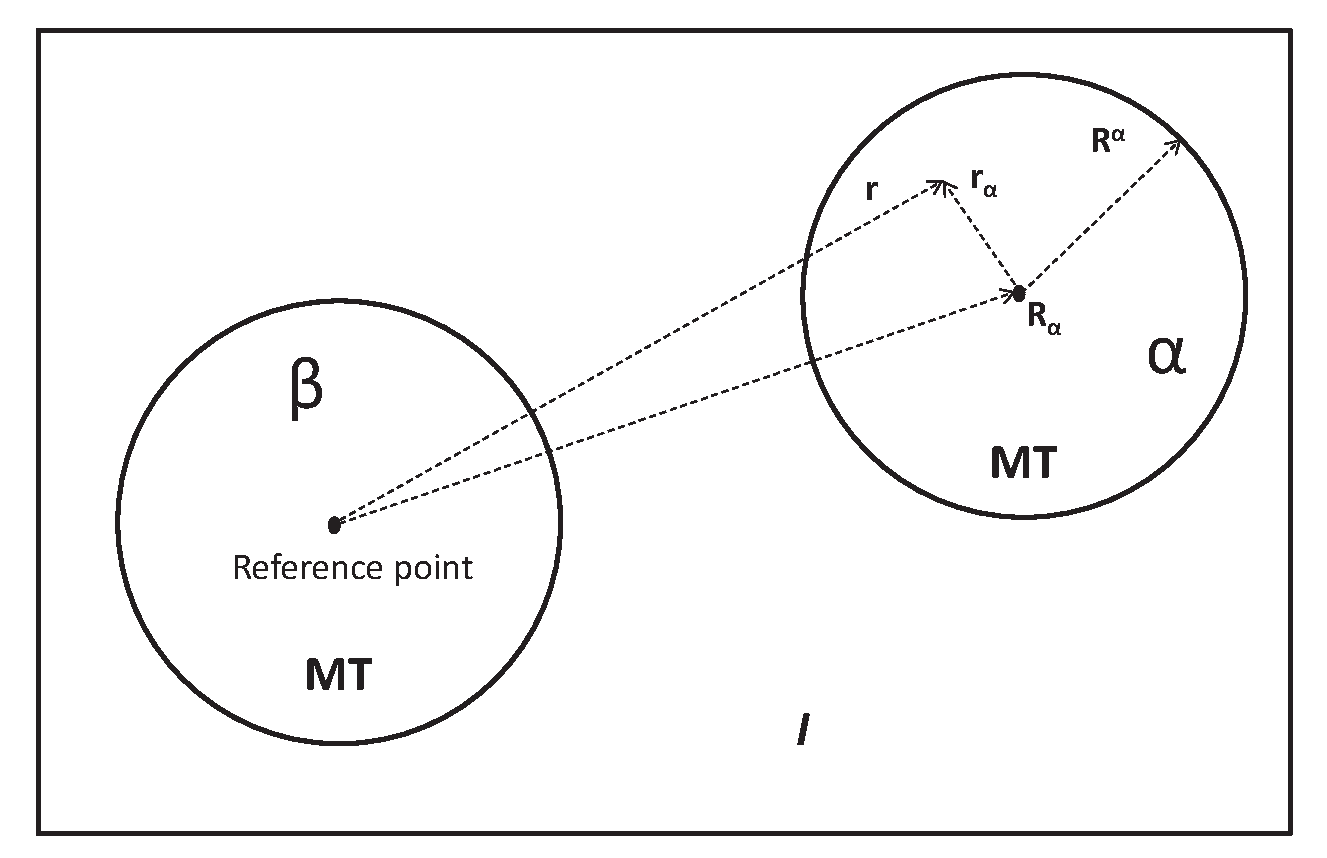
\includegraphics[scale=0.5]{unitcell.eps}
\caption{Partition of the unit cell.}
\label{ucuc}
\end{center}
\end{figure}

In \textbf{Fig. \ref{ucuc}}, one notices that unit cell is divided into MT spheres ($\alpha$, $\beta$) and an
$I$ region, where ${\textbf r = {\textbf R_{\alpha}}+{\textbf r_{\alpha}}}$ is guaranteed. The Rayleigh expansion formula yields

\begin{equation}
\expg<(\textbf {k}+\textbf{G})> = e^{i (\textbf {k}+\textbf{G}) \textbf{R}_{\alpha} } 4 \pi \sum\limits_{{\ell}}^{N_{\ell}} \sum\limits_{{m}}^{N_{m}} i^{\ell} \bessf< |\textbf{k}+\textbf{G}|> \sphfr<\ell{m}><r><> Y_{\ell{m}}(\widehat{\textbf{k}+\textbf{G}}).
\end{equation}
  
Therefore, the following equation is satisfied for each ${\ell}m$

\begin{equation}
A _{{\ell}m}^{\alpha} (\textbf {k}+\textbf{G})  u_{{\ell}}^{\alpha}(r_{\alpha})=  \frac{4 \pi }{\sqrt{\Omega}} e^{i (\textbf {k}+\textbf{G}) \textbf{R}_{\alpha} }  \sum\limits_{{\ell}}^{N_{\ell}} \sum\limits_{{m}}^{N_{m}} i^{\ell} \bessf< |\textbf{k}+\textbf{G}|> Y^{*}_{\ell{m}}(\widehat{\textbf{k}+\textbf{G}}).
\end{equation}

The main drawback about the APW method is that the wavefunction is energy-dependent (\textbf{Eq. \ref{ap2}}). It is time-consuming to calculate the exact energy.

\subsubsection{Linearized augmented plane wave method}
\noindent In order to decouple the energy from the wavefunction in the APW method, Andesen, Koelling and Arbman found out a way to separate them \cite{andersen1975linear, koelling1975use}. They noticed that the Taylor expansion of the radial function
on certain energy, which can be given as

\begin{equation}\label{ap3}
 u_{{\ell}}(r_{\alpha}, \epsilon) = u_{{\ell}}(r_{\alpha}, \epsilon_{\ell,\alpha}) + (\epsilon-\epsilon_{\ell,\alpha}) \dot{u}_{{\ell}}(r_{\alpha}, \epsilon_{\ell,\alpha}) + O((\epsilon-\epsilon_{\ell,\alpha})^2).
\end{equation}

Here, eigenvalue ($\epsilon$) is written without subscript and superscript. Thus, the basis function is re-defined as 

\begin{equation}\label{lap4}
\phi^{LAPW}_{\textbf{k}+\textbf{G}} (\textbf{r}) = 
\begin{cases} \frac {1}{\sqrt{\Omega}} e^{i(\textbf{k}+\textbf{G})\textbf{r}} & \quad \mbox{if $\textbf{r} \in {I} $}
\\
\sumg<\alpha>\sum\limits_{{\ell}m} f_{{\ell}{m}} (r_{\alpha},\textbf{k}+\textbf{G}, \epsilon_{\ell,\alpha}) Y_{{\ell}m}(\hat{\textbf{r}}_{\alpha})  & \quad \mbox{if $r_{\alpha} \in MT. $}\\ 
\end{cases}
\end{equation}

Here, $f_{{\ell}{m}} (r_{\alpha},\textbf{k}+\textbf{G}, \epsilon_{\ell,\alpha}) =  A _{{\ell}m}^{\alpha} (\textbf {k}+\textbf{G}) u_{{\ell}}(r_{\alpha}, \epsilon_{\ell,\alpha}) + B _{{\ell}m}^{\alpha} (\textbf {k}+\textbf{G}) \dot{u}_{{\ell}}(r_{\alpha}, \epsilon_{\ell,\alpha})$
. $A _{{\ell}m}^{\alpha} (\textbf {k}+\textbf{G})$ and $B _{{\ell}m}^{\alpha} (\textbf {k}+\textbf{G})$ are expansion coefficients, and $\dot{u}_{{\ell}}(r_{\alpha}, \epsilon_{\ell,\alpha} )$ is derivative of the radial 
function. Energy $\epsilon_{\ell,\alpha}$  is considered as pre-calculated parameter in \textbf{Eq. \ref{lap4}}. Actually, it is chosen by the middle of  each $\ell$-character band. Therefore this method is called linearized
augmented plane wave (LAPW) method.

Apparently, LAPW method is more suitable in reality, because the wavefunction is decoupled with energy. However it has to match for two parameters.
Fortunately, it still takes less time comparing with APW method. However, there is one drawback about this method, what if energy in the same ${\ell}$-character is different enough, 
which $\epsilon_{\ell,\alpha}$ is correct? These states are called as semi-core states, which exist in the actinides and the rare earth elements.

\subsubsection{Local orbitals}
In order to solve semi-core states problem, a new basis function is added in the LAPW method. it is defined as


\begin{equation}\label{lap5}
\phi^{LO}_{\textbf{k}+\textbf{G}}(\textbf{r}) = 
\begin{cases} 0 & \quad \mbox{if $\textbf{r} \in {I} $}
\\
(A _{{\ell}m}^{\alpha,LO}  u_{{\ell}}(r_{\alpha}, \epsilon_{\ell,\alpha}) + B _{{\ell}m}^{\alpha,LO}  \dot{u}_{{\ell}}(r_{\alpha}, \epsilon_{\ell,\alpha}) + C _{{\ell}m}^{\alpha,LO}  u_{{\ell}}(r_{\alpha}, \epsilon'_{\ell,\alpha})){Y_{{\ell}m}(\hat{\textbf{r}}_{\alpha})} & \quad \mbox{if $r_{\alpha} \in MT. $}\\ 
\end{cases}
\end{equation}
 

Here, $A _{{\ell}m}^{\alpha,LO}$, $B _{{\ell}m}^{\alpha,LO}$, and $C _{{\ell}m}^{\alpha,LO}$ can be obtained by normalization, as well as value and derivation on the sphere boundary to zero. The $\epsilon'_{\ell,\alpha}$ is
the chosen energy from semi-core state. This method is called as linearized augmented plane wave method plus local orbitals (LAPW+LO) method.


There is another method called augmented plane wave method plus local orbitals (APW+lo), which can solve the APW method efficiently. The 
basis function has two types: one is similar with APW method, but without the derivative terms, that is, $f_{{\ell}{m}} (r_{\alpha},\textbf{k}+\textbf{G}, \epsilon_{\ell,\alpha}) =  A _{{\ell}m}^{\alpha}(\textbf{k}+\textbf{G})u_{{\ell}}(r_{\alpha}, \epsilon_{\ell,\alpha})$; 
the other basis function is

\begin{equation}\label{lap6}
\phi^{lo}_\textbf{k+G} (\textbf{r}) = 
\begin{cases} 0 & \quad \mbox{if $\textbf{r} \in {I} $}
\\
(A _{{\ell}m}^{\alpha,lo}  u_{{\ell}}(r_{\alpha}, \epsilon_{\ell,\alpha}) + B _{{\ell}m}^{\alpha,lo}  \dot{u}_{{\ell}}(r_{\alpha}, \epsilon_{\ell,\alpha}) ){Y_{{\ell}m}(\hat{\textbf{r}}_{\alpha})} & \quad \mbox{if $r_{\alpha} \in MT. $}\\ 
\end{cases}
\end{equation}
 
Value of $A _{{\ell}m}^{\alpha,lo}$ and $B _{{\ell}m}^{\alpha,lo}$ are obtained by normalization, and local orbital has zero value at the muffin tin boundary. This method is not suitable for the calculations considering semi-core states.
However, it does increase the efficiency. Certainly, There are some types of basis function which can mix the advantages from mentioned methods.

\subsection{Effective potential}

\label{epote}
The potential in the FPLAPW method is also divided into two regions, the MT region and the $I$ region \cite{nordstrom2006planewaves}.
\begin{equation*}\label{lap7}
V(\textbf{r}) = 
\begin{cases} \sumg<{\textbf G}> V_{\textbf G} e^{i {\textbf G} {\textbf {r}  }} & \quad \mbox{if $\textbf{r} \in {I} $}
\\
 \sum_{{\ell}m} V_{{\ell}m}^{\alpha} (r_{\alpha}) Y_{{\ell}m}(\hat{{\textbf r}}_{\alpha})  & \quad \mbox{if $r_{\alpha} \in MT. $}\\ 
\end{cases}
\end{equation*}

\section{Dielectric function}
The dielectric function describes optical property of materials \cite{penn1962wave, fox2002optical}. Normally, it is written as $\varepsilon(\omega)$, which has two parts

\begin{equation}
 \varepsilon(\omega) = \varepsilon_1(\omega) + i \varepsilon_2(\omega).
\end{equation}

Here, $\varepsilon_1(\omega)$ denotes how much the material is polarized when an electric field is applied, and $\varepsilon_2(\omega)$ is related with absorption of the material. The imaginary part of interband contribution to the dielectric function is defined as

\begin{equation}\label{df2}
\varepsilon_2^{\alpha\beta} (\omega)= \frac{\hbar e^2}{\pi m^2\omega^2} \sum_{cv} \int d \textbf {k} <\Psi_{c{\textbf k}}|p^\alpha|\Psi_{v{\textbf k}}><\Psi_{v{\textbf k}}|p^\beta|\Psi_{c{\textbf k}}> (f(\varepsilon_{c \textbf k})-f(\varepsilon_{v \textbf k}))\delta(\varepsilon_{c {\textbf k}}-\varepsilon_{c{\textbf k}}-\omega).
\end{equation}

Here, $f$ is the Fermi distribution function,  $c$ and $v$ are indices of conduction band and valence band. The total imaginary part of dielectric function can be calculated when $c$ and $v$ run over all indices of 
the conduction bands and valence bands. Similarly, the interband contribution can be achieved by calculating single conduction band and single valence band.   

The real part of dielectric function can be calculated by Kramers-Kronig relations

\begin{equation}
 \varepsilon_1^{\alpha\beta} (\omega)= \delta_{\alpha\beta}+\frac{2}{\pi}\textbf{P}\int^{\infty}_{0} \frac{\omega'\varepsilon_2^{\alpha\beta}(\omega')}{\omega'^{2}-\omega^{2}} d\omega'.
\end{equation}

Here, $\textbf{P}$ the Cauchy principal value. The absorption coefficient can be obtained by the real part and imaginary part of dielectric function
\begin{equation}\label{czr852}
 \alpha^{ii}(\omega) = \frac{\sqrt{2}\omega}{c} \left[ \sqrt{{\varepsilon^{ii}_1(\omega)}^2+{\varepsilon^{ii}_2(\omega)}^2}-{\varepsilon^{ii}_1(\omega)} \right]^{1/2}.
\end{equation}

Here, \textbf{Eq. \ref{czr852}} equation is only valid for the diagonal of the tensor.

In this section, only some basic equations are covered when it is related to calculate the dielectric function. One can find more detailed description in Ref. \cite{ambrosch2006linear}.


\section{\textbf{k} $\cdot$ \textbf{p} method}
\label{kpmaa}

The energy band dispersion can be obtained exactly by using the $\bold k \cdot \bold p$ method in principle. The basic idea of this method is explained in this section based on Refs. \cite{voon2009kp, kane1966k}.

The non-relativistic Kohn-Sham equation (not in atomic units) is give as

\begin{equation}\label{kpse}
\Big( \frac {{\textbf p}^2} {2m_e} + V({\textbf r}) \Big) \wfbloch<n>< \bold k> = \epsilon_{n,\textbf{k}} \wfbloch<n><\bold k>.
\end{equation}

Here, $\textbf p$ is momentum operator, and the superscript "$KS$" is ignored compared with \textbf{Eq. \ref{aaa111}}. According to the Bloch theory, the wavefunction can be written as

\begin{equation}\label{1}
 \wfbloch<n><\bold k> = \expg<k> \ubloch<n><\bold k>.
\end{equation}

Here, $\ubloch<n><\bold k>$ is a function, which has the same periodicity as the potential. If substituting \textbf{Eq. \ref{1}} to \textbf{Eq. \ref{kpse}}, a new equation is derived as

\begin{equation}\label{kp1}
 \Big(  \frac{{\textbf p}^2}{2m_e} + V({\textbf r }) + \frac{{\hbar^2 {\textbf k}^2}}{2m_e} + \frac{{\hbar \textbf {kp}}}{m_e} \Big) \ubloch<n><\bold  k>  =  \epsilon_{n,\textbf{k}} \ubloch<n><\bold  k>.
\end{equation}

In \textbf{Eq. \ref{kp1}}, the Hamiltonian becomes $H_0 = {\textbf p}^2 / {2m_e} + V({\textbf r })$ when $\textbf k = \textbf 0$, the corresponding eigenvalue is $\epsilon_{n,\textbf{0}}$. 
Here, terms in $H_0$ can be seen as non-perturbation terms, and remaining terms are seen as perturbation terms. From the perturbation theory, the following equation can be obtained  

\begin{equation}
 \epsilon_{n,\textbf{k}} =  \epsilon_{n,\textbf{0}} + \frac{{\hbar^2 {\textbf k}^2}}{2m_e} + \frac{ \hbar^2}{m_{e}^2} \sum\limits_n^{N} \sum\limits_{n' \neq n}^{N} \frac{|<\ubloch<n><\bold 0>|{\textbf {kp}}|\ubloch<n'><\bold  0>>|^2}{\epsilon_{n,\textbf 0} - \epsilon_{n',\textbf 0}}.
\end{equation}

In the realistic implementation, the following derivation is exploited \cite{persson2007full}. Assume that the wavefunction and eigenvalue are obtained by some procedures on $\textbf{k}_0$ point. $\wfbloch<n><\bold{k}_0>$ is the corresponding wavefunction
and $\epsilon_{n,\textbf{k}_0}$ is the corresponding eigenvalue. Luttinger-Kohn function is given as

\begin{equation}\label{kp2}
\chikp<n><\textbf k> = \expg<(\bold k-\bold {k_0})>  \wfbloch<n><\textbf{k}_0>.
\end{equation}

The wavefunction on ${ \textbf k}$ point can be expanded by $\chikp<n><\textbf k> $, which is given as
\begin{equation}\label{kp3}
\wfbloch<n><\bold k> =  {\sum\limits_{j}^{N}} C_{n,j}^{\bold k} \chikp<j><\bold k>. 
\end{equation}

In \textbf{Eq. \ref{kp3}}, the wavefunction can be obtained if the coefficient $C_{n,j}^{\bold k}$ is obtained. Based on \textbf{Eq. \ref{kp3}} and  \textbf{Eq. \ref{kpse}}, the following equation is derived

\begin{equation}\begin{split}\label{5}
& {\sum\limits_{j}^{N}}  C_{n,j}^{\bold k} \left(  \Big(  \epsilon_{n,\textbf{k}_0} -  \epsilon_{n,\textbf{k}}  + \frac{{\hbar}^2}{2m_e} { (\bold {k}^2- \bold {k}_0^2)}    \Big) \delta_{j',j} + \frac{\hbar}{m_e} {(\bold {k}-\bold{k}_0)} {\overline{\textbf{p}}_{j',j}} \right ) = 0 \\
& {\overline{\textbf{p}}_{j',j}} = \langle \ubloch<j'><\textbf{k}_0>| {\textbf p} | \ubloch<j><\textbf{k}_0>  \rangle.
\end{split}
\end{equation}

\textbf{Eq. \ref{5}} can be simplified as
 
\begin{equation}\begin{split}\label{6}
& {\sum\limits_{j}} C_{n,j}^{\bold {k}} \left ( H_{j',j}-  \epsilon_{n,\textbf{k}} \delta_{j',j} \right ) =0 \\
& H_{j',j} = \Big(   \epsilon_{n,\textbf{k}_0}  + \frac{{\hbar}^2}{2m_e} { (\bold{k}^2-\bold{k}_0^2)}    \Big) \delta_{j',j} + \frac{\hbar}{m_e} {(\bold{k}-\bold{k}_0)} {\overline{\textbf{p}}_{j',j}}.
\end{split}
\end{equation}

Here, the coefficient $ C_{n,j}^{\bold k}$ and $\epsilon_{n,\textbf{k}}$ can be calculated. Therefore, the wavefunction on any ${ \textbf k}$ point can be obtained.


\section{Spin-orbit coupling}
\label{srasoc}

\subsection{Dirac equation}

Non-relativistic quantum mechanics has broad application. However, the non-relativistic quantum is not suitable to describe the system, where the velocity of electrons is near the one of light $c$. 
Therefore, Dirac introduced an equation, which is called Dirac equation applying for relativistic case \cite{thaller1992dirac, dirac1930principles}.

\noindent Dirac defined the Hamiltonian as
\begin{equation}\label{dirac}
{H}^{dirac} = c \boldsymbol{\alpha} \textbf{P} + \boldsymbol{\beta}m_ec^{2} + V.
\end{equation}

\noindent Here, $\textbf{P} = -i\hbar \nabla $ is the momentum operator, $V$ is the general potential, and $m_e$ is the mass of electron. 
 $\boldsymbol{\alpha}$ and $\boldsymbol{\beta}$ are $4 \times 4$ matrices, which are defined as
\begin{equation}
 \boldsymbol{\alpha} = \left( \begin{array}{cc}
 0 & \boldsymbol{\sigma}  \\
 \boldsymbol{\sigma} & 0   \end{array} \right),
\boldsymbol{\beta} = \left( \begin{array}{ccc}
\boldsymbol{I} & 0\\
0 & -\boldsymbol{I}\end{array} \right).
\end{equation}

\noindent Here, $\boldsymbol{I}$ is unit matrix. $\boldsymbol{\sigma}$ is Pauli matrix, which is given as

\begin{equation} 
\boldsymbol{\sigma} = (\boldsymbol{\sigma}_x \  \boldsymbol{\sigma}_y \  \boldsymbol{\sigma}_z )  
\end{equation}

\begin{equation}
\boldsymbol{\sigma}_x = \left( \begin{array}{cc}
0 & 1\\
1 & 0\end{array} \right),
\boldsymbol{\sigma}_y = \left( \begin{array}{ccc}
0 & -i\\
i & 0\end{array} \right),
\boldsymbol{\sigma}_z = \left( \begin{array}{ccc}
1 & 0\\
0 & -1\end{array} \right).
\end{equation}

\subsection{Derivation of spin-orbit coupling}

\noindent  Assume that $\Psi$ is the wavefunction of Hamiltonian in \textbf{Eq. \ref{dirac}}, which has four components \cite{thaller1992dirac, dirac1930principles}. However, it can be 
written with only two terms
\begin{equation}\label{diracwf}
\Psi = \left( \begin{array}{c}
\phi^{\uparrow} \\
\phi^{\downarrow} \\
\chi^{\uparrow} \\
\chi^{\downarrow} \end{array} \right),
 \Psi = \left(\begin{array}{c}
\phi \\               
\chi \end{array} \right).
\end{equation}

\noindent Here, $\phi$ includes the two terms of $\phi^{\uparrow}$ and $\phi^{\downarrow}$, and $\chi$ contains  $\chi^{\uparrow}$ and $\chi^{\downarrow}$.
Under the non-relativistic limit, $\phi$ is bigger than $\chi$ by the ratio of $v/c$. Here, $v$ and $c$ are velocities of electrons and light, respectively.
Therefore, the $\phi$ is considered as the large term and $\chi$ is the small one.

\noindent In order to derive the spin-orbit coupling term, we need to take use of the non-relativistic limit approximation ($v^2/c^2 << 1$). The time-independent Dirac equation is give as

\begin{equation}\label{diracse}
 E \Psi = (c \boldsymbol{\alpha} \textbf{P} + \boldsymbol{\beta}m_ec^{2} + V) \Psi.
\end{equation}

\noindent For convenience, the following equation is defined

\begin{equation}\label{dirace}
E^{\prime} = E - m_ec^2.
\end{equation}

\noindent Here, $E$ is the total energy, $m_ec^2$ and $E'$ are the rest mass energy and the remaining energy excluding the rest mass energy, respectively. Under the non-relativistic limit, 
$E'$ is far smaller than $m_ec^2$. The following equation is given when \textbf{Eq. \ref{diracwf}} and \textbf{Eq. \ref{dirace}} are put into \textbf{Eq. \ref{diracse}}

\begin{equation}
\begin{split}
&(E^{\prime} - V) \Phi - c \boldsymbol{\sigma} \textbf{P} \chi = 0\\                
&-c\boldsymbol{\sigma} \textbf{P} \Phi + (E^{\prime}+2m_ec^2-V)\chi = 0.
\end{split}
\end{equation}

\noindent To eliminate the $\chi$ (otherwise, it is the antiparticle problem), it ends up with the equation
  \begin{equation}\label{soc1212}
\Big(V + \frac{1}{2m_e} (\boldsymbol{\sigma} \textbf{P}) (1+\frac{E^{\prime}-V}{2m_ec^2})^{-1} (\boldsymbol{\sigma} \textbf{P}) \Big)\phi=E^{\prime}\phi.
\end{equation}

\noindent Here, ${E^{\prime}-V}$ is far smaller than ${2mc^2}$, therefore, taking advantage of the Taylor expansion of it,  as well as the following identites

\begin{equation}
\begin{split}
& [\textbf{P}, V ] = -i \hbar \triangledown V \\                
&(\boldsymbol{\sigma} \textbf{A} )(\boldsymbol{\sigma} \textbf{B}) = \textbf{A} \textbf{B} + i\boldsymbol{\sigma}[\textbf{A} \times \textbf{B}].
\end{split}
\end{equation}

The final equation is obtained under the non-relativistic limit

\begin{equation}\label{nonrela1}
E^{\prime} \phi = \Big(\frac{\textbf{P}^2}{2m_e} + V - \frac{\textbf{P}^4}{8 {m_e}^3 {c}^2}-\frac{i\hbar}{4{m_e}^2 {c}^2} (\nabla{V})\textbf{P}+\frac{\hbar}{4 m_e^2 c^2} \boldsymbol{\sigma}[\nabla{V} \times \textbf{P}]\Big) \phi.
\end{equation}

Furthermore, we can approximate the above equation to the simpler expression under spherical symmetry potential

\begin{equation}
 E^{\prime} \phi = \Big(\frac{\textbf{P}^2}{2m_e} +V - \frac{\textbf{P}^4}{8 {m_e}^3 {c}^2}-\frac{i\hbar}{4{m_e}^2 {c}^2} (\nabla{V})\textbf{P}+\frac{1}{2 m_e^2 c^2} \frac{1}{R} \frac{dV}{dR}\textbf{S}\textbf{L}\Big) \phi.
\end{equation}

\noindent Here, $\textbf{S} = {\hbar}{\boldsymbol{\sigma}}/2$ is the Pauli spinor, and $\textbf{L} = \textbf{R} \times \textbf{P}$ is the orbital
angular momentum operator. The terms of ${\textbf{P}^2}/(2m_e) + V$ is Schrödinger term,  ${\textbf{P}^4}/(8 {m_e}^3 {c}^2)$ and ${i\hbar} (\nabla{V})\textbf{P} /(4{m_e}^2 {c}^2)$  are the mass enhancement 
and Darwin term, respectively, both of them together is called the scalar relativistic approximation (SRA). The last term is the spin-orbit coupling (SOC) term. One has to
notice that the Darwin term is not hermitian operator, alternatively, $\nabla^2{V} /(8{m_e}^2 {c}^2)$ is suggested in the realistic implementation.

\textbf{Eq. \ref{nonrela1}} is only valid if the velocity of electrons is slower than the one of light. It is not true in the region which is close to the nucleus for heavy elements, where the relativistic effects
are relatively strong. Moreover, the Coulomb potential can be arbitrarily large negative energies in realistic situation as well. Therefore, there is another way to derive 
the spin-orbit coupling, which can overcome the mentioned disadvantages.

\textbf{Eq. \ref{soc1212}} can be rewritten as

\begin{equation}\begin{split}\label{soc001}
& \Big(V + (\boldsymbol{\sigma} \textbf{P}) \Big(\frac{c^2}{2m_ec^2-V}\Big)\Big(1+\frac{E^{\prime}}{2m_ec^2-V}\Big)^{-1} (\boldsymbol{\sigma} \textbf{P}) \Big)\phi \\
& \approx \Big( V + (\boldsymbol{\sigma} \textbf{P}) \Big(\frac{c^2}{2m_ec^2-V}\Big)(\boldsymbol{\sigma} \textbf{P}) \Big)\phi \\
& - (\boldsymbol{\sigma} \textbf{P}) \Big(\frac{c^2}{2m_ec^2-V}\Big)\Big(\frac{E^{\prime}}{2m_ec^2-V}\Big)^{-1} (\boldsymbol{\sigma} \textbf{P}) \Big)\phi + \cdots \\
& =E^{\prime}\phi.
\end{split}
\end{equation}

Here, the Taylor expansion is utilized. The zeroth order regular approximation (ZORA) Hamiltonian \cite{van1994relativistic, faas1995zora, van1996zero} is defined as
\begin{equation}\begin{split}\label{zora1}
& H^{zora} = V + (\boldsymbol{\sigma} \textbf{P}) \Big(\frac{c^2}{2m_ec^2-V}\Big)(\boldsymbol{\sigma} \textbf{P}) \\
& =  V + \textbf{P} \Big(\frac{c^2}{2m_ec^2-V}\Big)\textbf{P} + \frac{c^2}{(2m_ec^2-V)^2} \boldsymbol{\sigma}\cdot(\bigtriangledown V\times \textbf{P}).
 \end{split}
\end{equation}

The last term in \textbf{Eq. \ref{zora1}} is the spin-orbit coupling term.



\begin{comment}
\chapter{Results and discussion}

In this chapter, the major results for the licentiate thesis are discussed. The first one is parameterization of energy bands for CuIn{\textsubscript{1-$x$}}Ga{\textsubscript{$x$}}Se\textsubscript{2}
where $x$ = 0, 0.5, and 1. The second one is the calculation of the dielectric function spectra for the
CuIn{\textsubscript{0.5}}Ga{\textsubscript{0.5}}Se\textsubscript{2} by all electron and full-potential linearized augmented plane wave (FPLAPW) method, which is compared with experimental results.
Moreover, the probable electronic origins of the critical point (CP) features are discussed as well.

\section{Parameterization of energy bands for CIGS}

\subsection{Parameterization method}
The curvature of energy bands is often demonstrated by the effective electron and hole masses. Generally, the parabolic energy dispersion, also named parabolic band approximation (pba),
is assumed to represent the shape of the energy bands

\begin{equation}\begin{split}\label{parabolic}
& E_{j}^{pb}(\textbf{k}) = E_{j}(\textbf{0}) \pm \left[ \frac{\widetilde{\textbf{k}}_{x}^{2}+\widetilde{ \textbf{k}}_{y}^{2}}{m_{j}^{\perp}} + \frac{\widetilde{\textbf{k}}_{z}^{2}}{m_{j}^{\parallel}} \right] \\
& \widetilde{\textbf{k}}_{\alpha}^{2} = \frac{\hbar^2 {\textbf{k}}_{\alpha}^{2}}{2e}, \textrm{where}\  \alpha = x, y, \textrm{and}\  z.
\end{split}
\end{equation}

Here, $m_{j}^{\perp}$ and $m_{j}^{\parallel}$ are transverse electron masses and longitudinal electron masses, respectively. Parameters in \textbf{Eq. \ref{parabolic}} to describe the parabolic energy dispersions of the lowest
conduction band (CB) and the three uppermost valence bands (VBs) in the vicinity of the $\Gamma$-point are given in \textbf{Table \ref{pm1}}.

\begin{table}[H]
\centering
 \captionsetup{width=1\textwidth}
\scalebox{0.9}{
 \begin{tabular}{c l l l l l l l l l l l l }
\hline
 &\multicolumn{4}{c}{CuInSe\textsubscript{2}}&\multicolumn{4}{c}{CuIn\textsubscript{0.5}Ga\textsubscript{0.5}Se\textsubscript{2}}&\multicolumn{4}{c}{CuGaSe\textsubscript{2}}\\
\cline{2-13}
 Parameters & $c$1 & $v$1 & $v$2 & $v$3 & $c$1 & $v$1 & $v$2 & $v$3 & $c$1 & $v$1 & $v$2 & $v$3\\
\hline\hline
$E_j(\textbf{0})$ [eV]    &1.04	 &0	&0.01	&0.19	&1.33	&0	&0.02	&0.2	&1.67	&0	&0.08	&0.26\\
$m_j^{\bot}$      [$m_0$] &0.08	 &0.14	&0.25	&0.27	&0.10	&0.40	&0.17	&0.29	&0.13	&0.47	&0.20	&0.29 \\
$m_j^{||}$        [$m_0$] &0.09  &0.66	&0.12	&0.28	&0.11	&0.14	&0.61	&0.40	&0.13	&0.15	&0.61	&0.49 \\
\hline
\end{tabular}}
\caption {Parameters in \textbf{Eq. \ref{parabolic}} for {CuInSe\textsubscript{2}}, {CuIn\textsubscript{0.5}Ga\textsubscript{0.5}Se\textsubscript{2}}, and {CuGaSe\textsubscript{2}}. $E_{v1}(\textbf{0})$ is the valence band maximum (VBM) and $E_{c1}(\textbf{0})$ is the fundamental band-gap energy $E_g$.}\label{pm1}
\end{table}

 
Unfortunately, these effective masses are only valid around the considered {\textbf k} point, which is not suitable to describe the non-parabolic away from this {\textbf k} point. However, the accurate shape of energy bands is 
important when one simulates and analyzes the electron transport or band filling.

In this work, we have parameterized the three uppermost VBs and the lowest CB for the materials of CuInSe\textsubscript2, CuIn\textsubscript{0.5}Ga\textsubscript{0.5}Se\textsubscript{2}, 
and CuGaSe\textsubscript{2}. This parameterization is based on results from FPLAPW calculations. Normally, the \textbf{k $\cdot$ p} method is utilized to 
parameterize the energy bands. However, the energy dispersions of CuIn{\textsubscript{1-$x$}}Ga{\textsubscript{$x$}}Se\textsubscript{2}
where $x$ = 0, 0.5, and 1 are rather complex due to the crystal-field interaction and the spin-orbit coupling. Therefore, the regular \textbf{k $\cdot$ p} method is not sufficient 
to describe the energy bands. We manage to extend the \textbf{k $\cdot$ p} expression to higher orders, which is called full band parameterization (fbp) in the following text. The fbp is valid around 0.5 eV below VBM and 0.5 eV 
above the conduction band minimum (CBM). The explicit equation is given as

\begin{equation}\label{nonparabolic}
\begin{split}
& \small E_j(\textbf{k}) = E_{j}^{pb}(\textbf{k}) + E_j^0 + \Delta_{j,1} \left( \delta_{j,1}^2 \left( \frac{\widetilde{\textbf{k}}_{x}^{4}+\widetilde{ \textbf{k}}_{y}^{4}}{m_{0}^{2}} \right) + \delta_{j,2}^2 \left( \frac{\widetilde{\textbf{k}}_{x}^{2}\widetilde{\textbf{k}}_{y}^{2}}{m_{0}^2} \right) + 1 \right)^{1/2} \\
& \small + \Delta_{j,2} \left( \delta_{j,3}^3 \left( \frac{\widetilde{\textbf{k}}_{x}^{6}+\widetilde{ \textbf{k}}_{y}^{6}}{m_{0}^{3}} \right) + \delta_{j,4}^3 \left( \frac{\widetilde{\textbf{k}}_{x}^{2}\widetilde{\textbf{k}}_{y}^{4} + \widetilde{\textbf{k}}_{x}^{4}\widetilde{\textbf{k}}_{y}^{2}}{m_{0}^3} \right) + 1 \right)^{1/3} \\
& \small + \Delta_{j,3} \left( \delta_{j,5}^2 \left( \frac{\widetilde{\textbf{k}}_{z}^{4}}{m_0^2} \right) + 1 \right)^{1/2} + \Delta_{j,4} \left( \delta_{j,6}^3 \left( \frac{\widetilde{\textbf{k}}_{z}^{6}}{m_0^3} \right) + 1 \right)^{1/3} \\
& \small + \Delta_{j,5} \left( \delta_{j,7}^2 \left( \frac{\widetilde{\textbf{k}}_{x}^{2}\widetilde{\textbf{k}}_{z}^{2} + \widetilde{\textbf{k}}_{y}^{2}\widetilde{\textbf{k}}_{z}^{2}}{m_{0}^2} \right) + 1 \right)^{1/2} \\
& \small + \Delta_{j,6} \left( \delta_{j,8}^3 \left( \frac{\widetilde{\textbf{k}}_{x}^{4}\widetilde{\textbf{k}}_{z}^{2} + \widetilde{\textbf{k}}_{y}^{4}\widetilde{\textbf{k}}_{z}^{2}}{m_{0}^3} \right) + \delta_{j,9}^3 \left( \frac{\widetilde{\textbf{k}}_{x}^{2}\widetilde{\textbf{k}}_{z}^{4} + \widetilde{\textbf{k}}_{y}^{2}\widetilde{\textbf{k}}_{z}^{4}}{m_{0}^3} \right) + \delta_{j,10}^3 \left( \frac{\widetilde{\textbf{k}}_{x}^{2}\widetilde{\textbf{k}}_{y}^{2}\widetilde{\textbf{k}}_{z}^{2}}{m_{0}^3} \right) +1 \right)^{1/3}.
\end{split}\end{equation}

Here,  $E_j^0$, $\Delta_{j,n}$, and $\delta_{j,m}$ are fitting parameters (see \textbf{Table. \ref{nonpara}}), ${m_0}$ is the electron rest mass. In \textbf{Eq. \ref{nonparabolic}}, each term represents one parabolic dispersion, the
higher order terms describe the larger wave vectors away from $\Gamma$ point. Unfortunately, the complex energy dispersions requires many fitting parameters. However, the conduction band needs less fitting parameters.


 \begin{sidewaystable}
 \captionsetup{width=1\textwidth}
\scalebox{0.8}{
 \begin{tabular}{c l l l l l l l l l l l l }
\hline
 &\multicolumn{4}{c}{CuInSe\textsubscript{2}}&\multicolumn{4}{c}{CuIn\textsubscript{0.5}Ga\textsubscript{0.5}Se\textsubscript{2}}&\multicolumn{4}{c}{CuGaSe\textsubscript{2}}\\
\cline{2-13}
 Parameters & $c$1 & $v$1 & $v$2 & $v$3 & $c$1 & $v$1 & $v$2 & $v$3 & $c$1 & $v$1 & $v$2 & $v$3\\
\hline\hline
$E_j^0$    [eV]              &\ \enspace0.533&$-$0.299           &$-$0.230         &$-$0.608        &\ \enspace0.569   &$-$1.045         &$-$1.261          &$-$0.669        &\ \enspace0.920   &\ \enspace10.580    &$-$0.492         &$-$2.513\\
$\bigtriangleup_{j,1}$  [eV] &$-$0.295       &\ \enspace0.006	 &$-$0.002         &$-$0.021        &$-$0.230          &\ \enspace0.106  &\ \enspace1.321   &$-$0.026        &$-$0.454          &\ \enspace0.116     &\ \enspace1.284  &\ \enspace1.194 \\
$\bigtriangleup_{j,2}$  [eV] &\ \enspace0    &\ \enspace0.098	 &\ \enspace0.104  &\ \enspace0.308 &\ \enspace0       &\ \enspace0.002  &\ \enspace0.096   &\ \enspace0.386 &\ \enspace0       &$-$10.771           &$-$0.837         &$-$0.024 \\
$\bigtriangleup_{j,3}$  [eV] &$-$0.242       &\ \enspace0.018	 &\ \enspace0.124  &$-$0.025        &$-$0.293          &\ \enspace0.937  &$-$0.017          &$-$0.838        &$-$0.419          &\ \enspace0.088     &\ \enspace0.347  &$-$0.303 \\
$\bigtriangleup_{j,4}$  [eV] &\ \enspace0    &\ \enspace0.188    &\ \enspace0.076  &\ \enspace0.238 &\ \enspace0       &\ \enspace0.021  &\ \enspace0.163   &\ \enspace0.789 &\ \enspace0	&\ \enspace0.076     &$-$0.051         &\ \enspace0.608 \\
$\bigtriangleup_{j,5}$  [eV] &$-$0.016       &$-$0.048           &\ \enspace0.001  &$-$0.009        &$-$0.046          &\ \enspace0.001  &\ \enspace0.011   &\ \enspace0.37  &$-$0.047          &\ \enspace0.022     &\ \enspace0.274  &\ \enspace0.374 \\
$\bigtriangleup_{j,6}$  [eV] &\ \enspace0    &\ \enspace0.037    &$-$0.073         &\ \enspace0.117 &\ \enspace0       &$-$0.022         &$-$0.313          &$-$0.012        &\ \enspace0       &$-$0.111            &$-$0.525         &$-$4.362 \\
$\delta_{j,1}$   [eV\textsuperscript{$-$1}]      &\ \enspace30.669	&\ \enspace952           &\ \enspace2304.147   &\ \enspace94.139  &\ \enspace27.157   &\ \enspace5.517     &\ \enspace 1.029  &\ \enspace57.007  &\ \enspace11.865   &\ \enspace10.526     &\ \enspace9.269   &\ \enspace   3.839 \\
$\delta_{j,2}$   [eV\textsuperscript{$-$1}]      &\ \enspace47.374	&\ \enspace1754.386      &\ \enspace4587.156   &\ \enspace220.556 &\ \enspace44.506   &\ \enspace13.61     &\ \enspace0.413   &\ \enspace153.435 &\ \enspace20.262   &\ \enspace28.545     &\ \enspace21.582  &\ \enspace   6.232 \\
$\delta_{j,3}$   [eV\textsuperscript{$-$1}]      &\ \enspace0	        &\ \enspace3.97          &\ \enspace72.296     &\ \enspace11.746  &\ \enspace0	      &\ \enspace487.805   &\ \enspace46.95   &\ \enspace8.489   &\ \enspace0	     &\ \enspace0.131      &\ \enspace9.116   &\ \enspace  59.625 \\
$\delta_{j,4}$   [eV\textsuperscript{$-$1}]      &\ \enspace0	        &\ \enspace3.688	 &\ \enspace123.274    &\ \enspace18.078  &\ \enspace0	      &\ \enspace1128.668  &\ \enspace72.844  &\ \enspace13.509  &\ \enspace0	     &\ \enspace0.126      &\ \enspace21.328  &\ \enspace 148.516 \\
$\delta_{j,5}$   [eV\textsuperscript{$-$1}]      &\ \enspace31.852	&\ \enspace6.041	 &\ \enspace56.004     &\ \enspace64.137  &\ \enspace21.124   &\ \enspace1.314     &\ \enspace247.158 &\ \enspace7.921   &\ \enspace12.978   &\ \enspace7.709      &\ \enspace12.141  &\ \enspace   8.014 \\
$\delta_{j,6}$   [eV\textsuperscript{$-$1}]      &\ \enspace0	        &\ \enspace3.134	 &\ \enspace6.1	       &\ \enspace12.031  &\ \enspace0	      &\ \enspace267.523   &\ \enspace29.076  &\ \enspace8.743   &\ \enspace0	     &\ \enspace64.185     &\ \enspace66.808  &\ \enspace   5.309 \\
$\delta_{j,7}$   [eV\textsuperscript{$-$1}]      &\ \enspace222.641     &\ \enspace37.004	 &\ \enspace3846.154   &\ \enspace206.148 &\ \enspace79.879   &\ \enspace3322.259  &\ \enspace212.902 &\ \enspace16.836  &\ \enspace76.319   &\ \enspace236.742    &\ \enspace16.24   &\ \enspace   5.092 \\
$\delta_{j,8}$   [eV\textsuperscript{$-$1}]      &\ \enspace0	        &\ \enspace12.647	 &\ \enspace16.269     &\ \enspace6.982   &\ \enspace0	      &\ \enspace92.954    &\ \enspace4.885   &\ \enspace57.89   &\ \enspace0	     &\ \enspace31.947     &\ \enspace6.71    &\ \enspace   1.209 \\
$\delta_{j,9}$   [eV\textsuperscript{$-$1}]      &\ \enspace0	        &\ \enspace61.565	 &\ \enspace33.169     &\ \enspace34.114  &\ \enspace0	      &\ \enspace118.064   &\ \enspace0	      &\ \enspace273.4   &\ \enspace0        &\ \enspace34.784     &\ \enspace4.831   &\ \enspace   1.394 \\
$\delta_{j,10}$  [eV\textsuperscript{$-$1}]      &\ \enspace0	        &\ \enspace46.679	 &\ \enspace31.275     &\ \enspace32.237  &\ \enspace0	      &\ \enspace110.327   &\ \enspace6.074   &\ \enspace153.523 &\ \enspace0	     &\ \enspace40.765     &\ \enspace5.243   &\ \enspace   2.124 \\
\hline
\end{tabular}}
\caption {Parameters in \textbf{Eq. \ref{nonparabolic}} to describe the non-parabolic contribution to the energy dispersions $E\textsubscript{j}(\textbf{k})$ of the lowest CB and the three uppermost VBs. The notation of the energy 
bands ($j$ = $c1$, $v1$, $v2$, and $v3$) refers to a spin-independent band indexing, where $c1$ represents the bottommost CB and $v1$ represents the topmost valence band (VB).}\label{nonpara}
\end{sidewaystable}


\subsection{Non-parabolicity properties}

The fbp of {CuIn\textsubscript{1-\textit{x}}Ga\textsubscript{\textit{x}}Se\textsubscript{2}} where $x$ = 0, 0.5, and 1 are plotted compared with the pba (\textbf{Eq. \ref{parabolic}}) as well as the calculations based 
on the FPLAPW method.

\begin{figure}[H]
    \begin{center}
            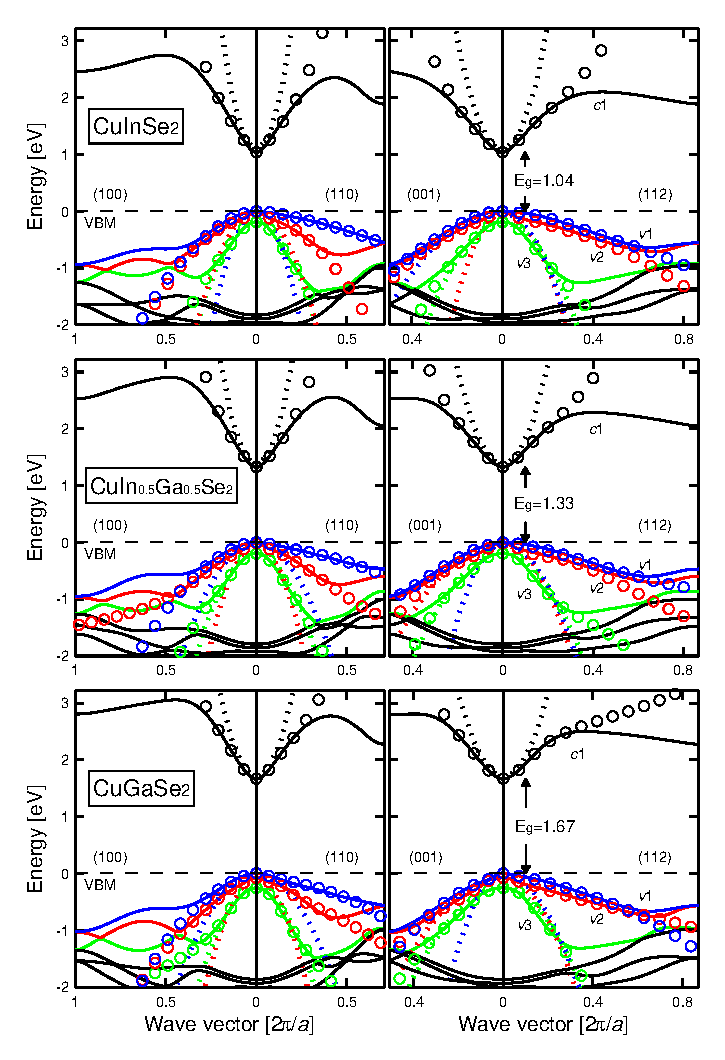
\includegraphics[width=0.45\textwidth,clip]{paper2figure1}
            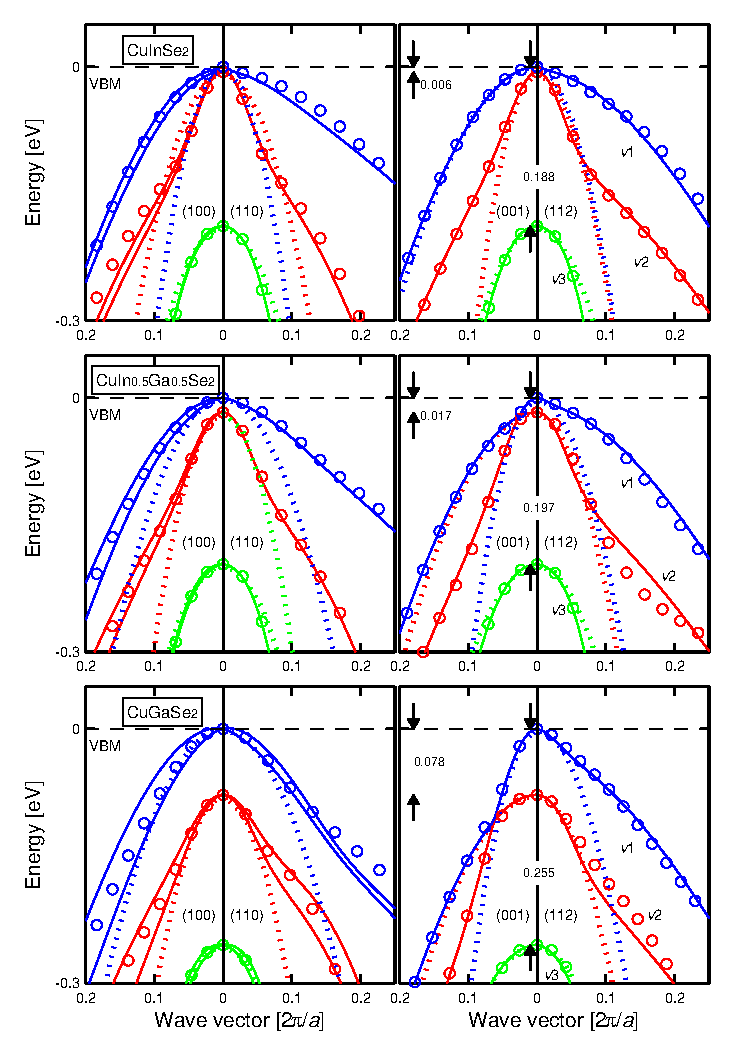
\includegraphics[width=0.46\textwidth,clip]{paper2figure2}
     \end{center}
    \caption{ Left panel: Electronic band structure along four directions. The circles are the results of the full band parameterization (fbp), and the dotted lines represent the parabolic band approximation (pba). Righ panel: The 
              close-up of left panel for the valence bands close to $\Gamma$ point.}      
    \label{bandstruct}
\end{figure}

In \textbf{Fig. \ref{bandstruct}}, the fbp can describe the energy below VBM around 0.5 eV accurately, and around 0.5 eV above the CB minimum (CBM) as well. However, the pba is only
valid below VBM around $-$4, $-$10, and $-$40 meV for the CuInSe\textsubscript2, CuIn\textsubscript{0.5}Ga\textsubscript{0.5}Se\textsubscript{2}, and CuGaSe\textsubscript{2}, respectively. Since the lowest conduction band
is more parabolic, therefore, the less fitting parameters are expected (see \textbf{Table \ref{nonpara}}).

To further utilize this parameterization method, the energy dispersions of the lowest CB and the three uppermost VBs are parameterized for kesterite and stannite Cu\textsubscript{2}ZnSnS\textsubscript{4}
and Cu\textsubscript{2}ZnSnSe\textsubscript{4} as well. It works as good as CuInSe\textsubscript2, CuIn\textsubscript{0.5}Ga\textsubscript{0.5}Se\textsubscript{2}, and CuGaSe\textsubscript{2}. Therefore, this parameterization method
can be utilized to other materials potentially.

\begin{figure}[H]
 \captionsetup{width=1\textwidth}
    \begin{center}
            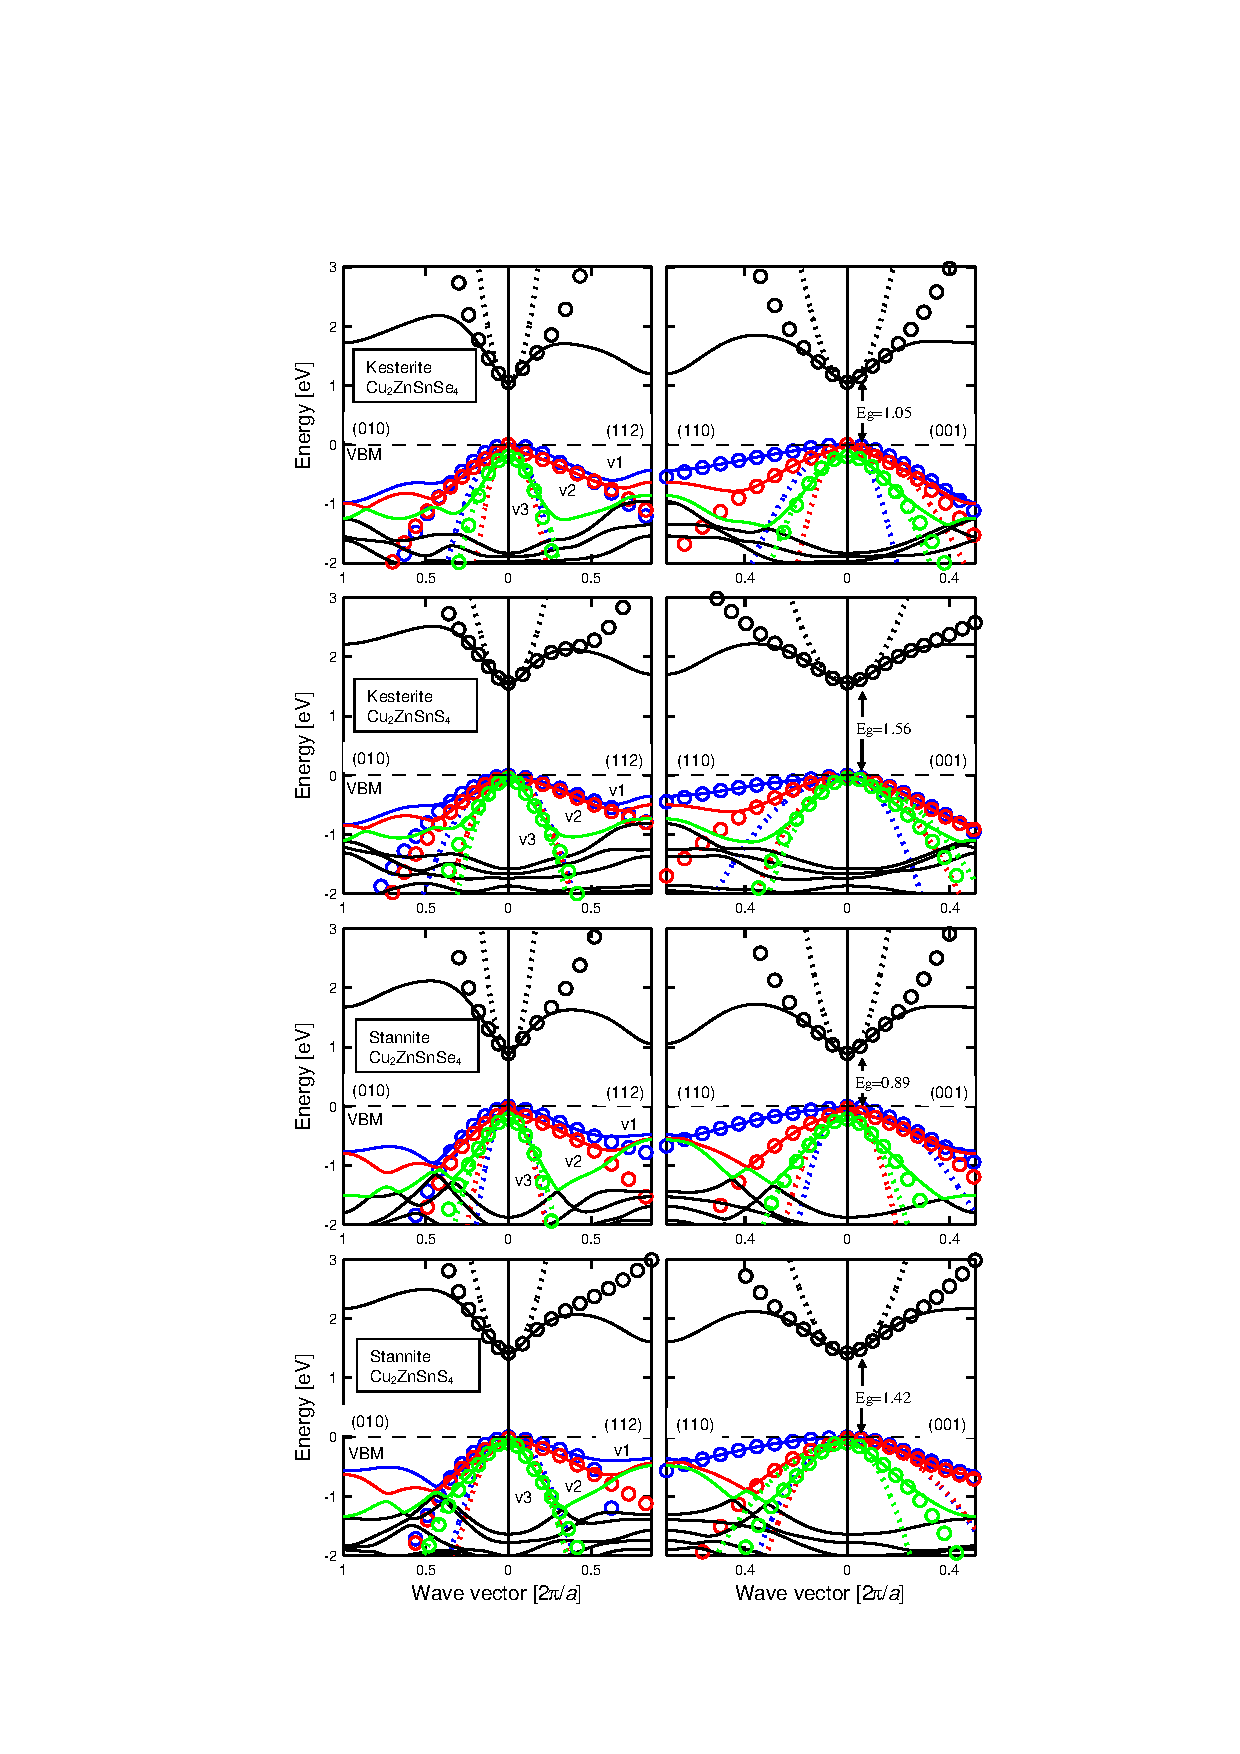
\includegraphics[width=1\textwidth,clip]{bandstr}
     \end{center}
    \caption{Left panel: electronic band structure for the kesterite structures of Cu\textsubscript{2}ZnSnS\textsubscript{4} and Cu\textsubscript{2}ZnSnSe\textsubscript{4}. Right panel: electronic band structure of the stannite structures of Cu\textsubscript{2}ZnSnS\textsubscript{4} and Cu\textsubscript{2}ZnSnSe\textsubscript{4}. The circles are the results based on the fbp, and the dotted lines represent results based on the pba. }      
    \label{bandstruct1}
\end{figure}


In order to demonstrate the anisotropic and non-parabolic of energy bands further, the constant energy surface $S_j(E)$ is determined for CuInSe\textsubscript{2} and CuGaSe\textsubscript{2}.

\begin{figure}[H]
    \begin{center}
            \includegraphics[width=0.46\textwidth,clip]{fermi_sphere_cii}
           % \includegraphics[width=0.4\textwidth,clip]{fermi_sphere_cig}
            \includegraphics[width=0.4\textwidth,clip]{fermi_sphere_cgg}
     \end{center}
    \caption{Left panel: constant energy surfaces for the three uppermost VBs and the lowest CB for the energies E = 1 meV. Right panel: constant energy surfaces for the three uppermost
    VBs and the lowest CB for the energies E = 200 meV.}
    \label{cse}
\end{figure}

In \textbf{Fig. \ref{cse}}, it is near to $\Gamma$ point when it refers to 1 meV; it is far away the $\Gamma$ point when it refers to 200 meV.
One notices that the pba is proper to describe the energy bands close to the $\Gamma$ point, and it is ellipsoidal shaped sphere. For example,
for the topmost VB ($v_1$) of CuInSe\textsubscript{2}, the constant energy surface is ellipsoidal in the vicinity of the $\Gamma$ point since the effective
masses are anisotropic ($m_{v1}^{\perp}$ = 0.14$m_0$ and $m_{v1}^{\parallel}$ = 0.66$m_0$ in \textbf{Table \ref{pm1}}). However, the constant energy surface becomes non-ellipsoidal when the energies 
is far away from $\Gamma$ point. For example, for the same band, the constant energy surface is not ellipsoidal shape at all when the energies goes up to 200 meV. It also implies that it is not correct to consider the constant 
effective mass. The change is relatively small for the CB.

\subsection{Application of the full band parameterization}

The parameterized energy bands can be exploited to reveal the detailed information near the VB and CB edged. In this section, the effective masses, density-of-states (DOS), Fermi level, and carrier concentration are calculated based on
fbp. In comparison with the results based on pba, all of the corresponding results are calculated with the pba as well.  

The effective masses are \textbf{k}-independent for the pba, which is not fully correct due to the non-parabolicity and anisotropy of the energy bands.  The effective masses tensors are calculated numerically by 
$m_j(\textbf{k}) = \pm \hbar^2/(\partial^2 E_j(\textbf{k})/\partial\textbf{k}^2) \ \textrm{where}\  j = c1, v1, v2, \textrm{and}\  v3.$


\begin{figure}[H]
    \begin{center}
            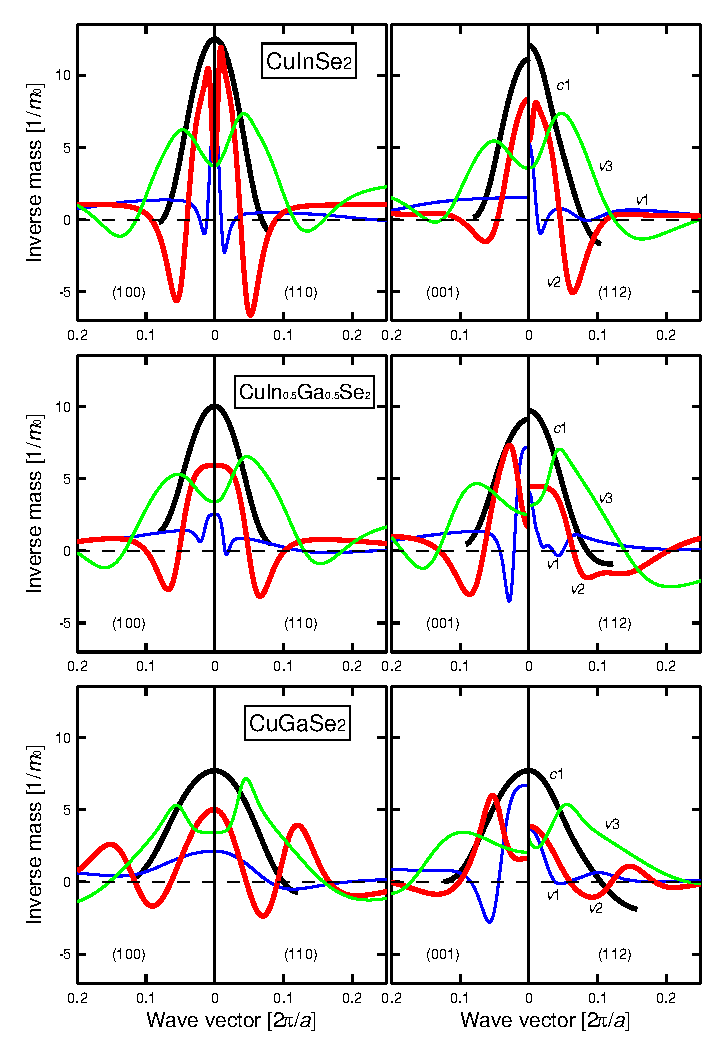
\includegraphics[width=0.43\textwidth,clip]{paper1figure3}
     \end{center}
    \caption{ Inverse of the effective electron and hole masses in the four symmetry directions for the {CuIn\textsubscript{1-\textit{x}}Ga\textsubscript{\textit{x}}Se\textsubscript{2}} ($x$ = 0, 0.5, and 1).}      
    \label{inversemessf}
\end{figure}

In \textbf{Fig. \ref{inversemessf}}, it demonstrates that the energy bands of {CuIn\textsubscript{1-\textit{x}}Ga\textsubscript{\textit{x}}Se\textsubscript{2}} ($x$ = 0, 0.5, and 1) are strong non-parabolic, since the effective masses should be constant in the pba along each symmetry direction. The effective hole masses of the two 
topmost VBs are strong anisotropy close to the $\Gamma$ point. However, the electron masses of conduction bands are rather isotropic ($m_{c1}^{100}(\textbf{0}) \approx m_{c1}^{110}(\textbf{0}) \approx m_{c1}^{001}(\textbf{0}) 
\approx m_{c1}^{112}(\textbf{0})$). Hole masses of CuGaSe\textsubscript{2} vary somewhat less compared with those of CuInSe\textsubscript{2} because CuGaSe\textsubscript{2} has larger split between the VBs. The inverse of the mass 
are presented in order to better visibility.



In order to further analyze the impact of non-parabolicity and anisotropy of the energy bands, the DOS is calculated based on fba and pba. The DOS in $j$th band is defined as

\begin{equation}\label{dosj}
 g_j(E)=\frac{1}{\Omega} \sum\limits_{\textbf{k}} 2 \delta (E-E_j(\textbf{k})) = \frac{1}{4\pi^3} \int \limits_{E_j(\textbf{k}) = E} \frac{dS(\textbf{k})}{|\bigtriangledown_\textbf{k} E_j(\textbf{k})|}.
\end{equation}
 
Here, $E_j(\textbf{k}) = E$ is the $\textbf{k}$ space surface with constant energy $E$, and the $\bigtriangledown_\textbf{k} E_j(\textbf{k})$ is the gradient of the energy dispersion.
In the case of the pba, \textbf{Eq. \ref{dosj}} can be written as

\begin{equation}\label{dosjp}
 g_j^{pba}(E) = \frac{1}{2\pi^2} \big(\frac{2m_j^{DOS}}{\hbar^2}\big)^{3/2} \sqrt{|E-E_j(\textbf{0})|}.
\end{equation}
 
Here, the DOS mass $m_j^{DOS}$ is equal to $\big( m_j^{\perp}m_j^{\perp}m_j^{\parallel} \big)^{1/3}$, which represents the extent of filling the specific band with free carriers to certain energy. 
In order to take advantage of the simple \textbf{Eq. \ref{dosjp}} for the non-parabolic energy bands, the energy-dependent DOS mass ($m_{v/c}^{DOS}$), which contains the non-parabolicity and anisotropy of the band dispersion, 
is defined as

\begin{equation}\label{dosmass}
 g_{v/c}(E) = \sum\limits_j g_j(E) = \frac{1}{2\pi^2} \big(\frac{2m_{v/c}^{DOS}(E)}{\hbar^2}\big)^{3/2} \sqrt{|E-E_{v1/c1}(\textbf{0})|}.
\end{equation}

Here, the energy-dependent DOS mass $m_{v/c}^{DOS}(E)$ contains the non-parabolicity and anisotropy of the band dispersion.


 \begin{figure}[H]
 \centering
  %\begin{center}
            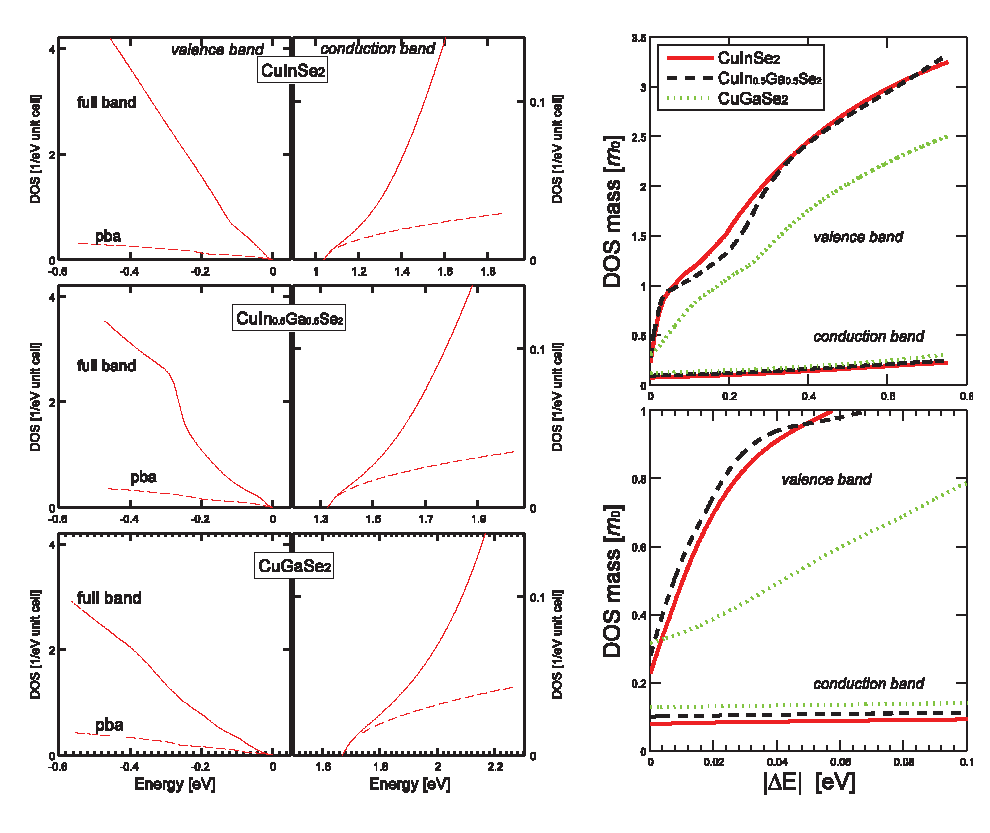
\includegraphics[width=0.7\textwidth,clip]{JAP2}
  %   \end{center}
    \caption{Left panel: total DOS of the VBs and CB. The solid lines show the results based on the fbp, and the dashed lines represent the results based on the pba. Right panel: The DOS mass $m_{v/c}^{DOS}$ is 
    calculated from \textbf{Eq. \ref{dosmass}}. }
   \label{dost}
\end{figure}


Left panel in \textbf{Fig. \ref{dost}} demonstrates that the non-parabolicity of the bands strongly affect the DOS dispersions. The difference is remarkable. The fbp always generates larger DOS, the reason is that the non-parabolic 
energy bands are more flat than parabolic bands. Right panel in \textbf{Fig. \ref{dost}} demonstrates that the DOS masses of {CuIn\textsubscript{1-\textit{x}}Ga\textsubscript{\textit{x}}Se\textsubscript{2}} ($x$ = 0, 0.5, and 1) is strong energy dependence with the VB DOS mass, which proves further the importance of considering 
non-parabolicity and anisotropy of the energy bands, especially for the VBs. For example, the effective mass of topmost VB for CuInSe\textsubscript{2} is around 0.23 $m_0$ close to the $\Gamma$ point, which goes up to
around 1.00 $m_0$ when $E$ is around 0.1 eV. \  However, the change in the CB DOS mass is subtle, but also goes up to 2$-$3 times with respect to the value around $\Gamma$ point.


\begin{comment}
 \begin{figure}[H]
 \centering
  %\begin{center}
            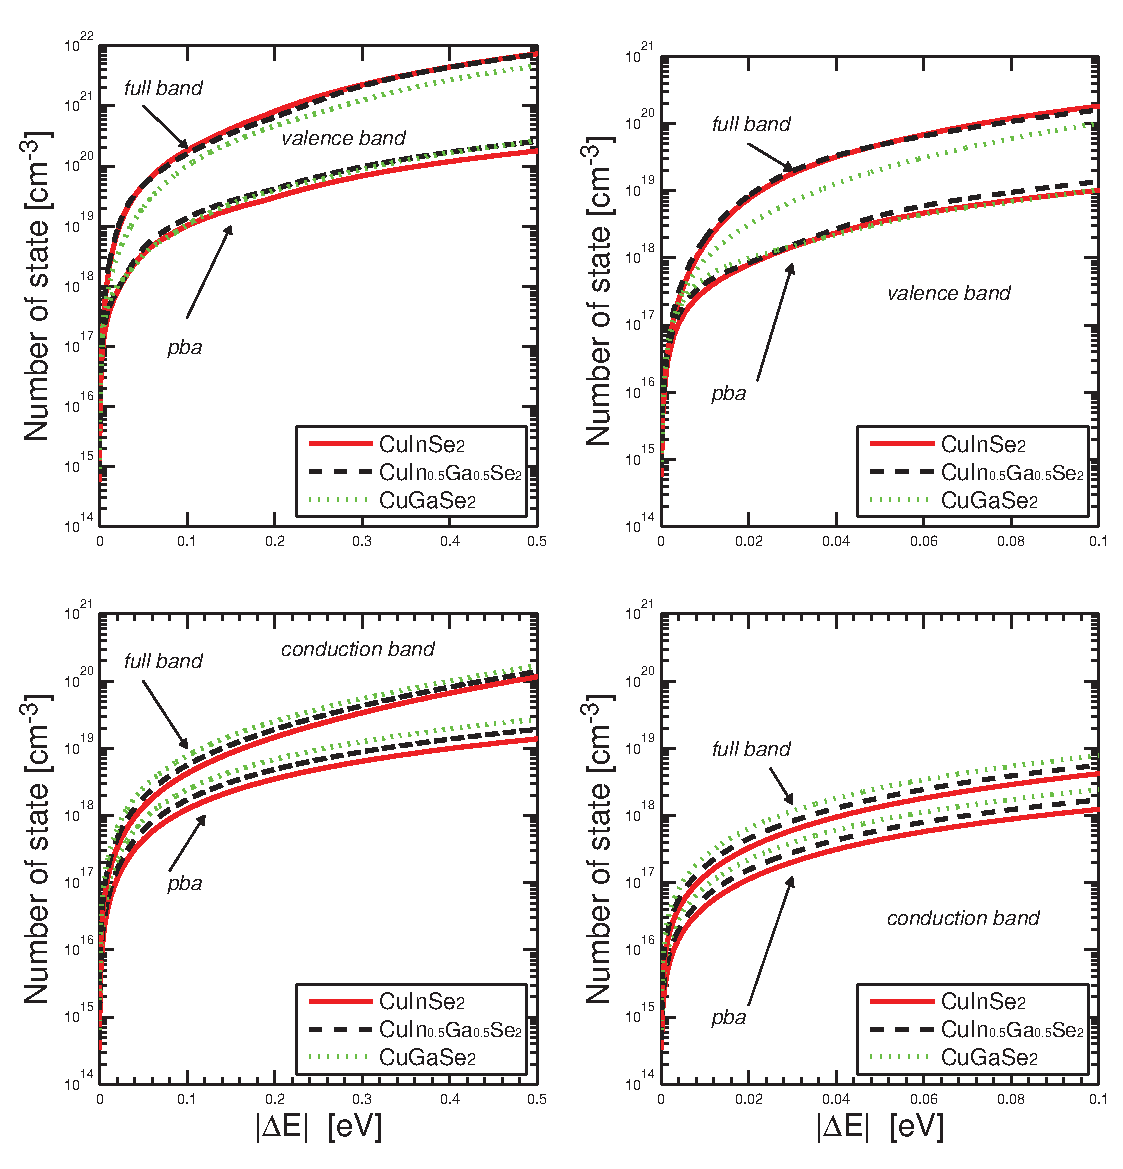
\includegraphics[width=0.7\textwidth,clip]{paper2fig5}
  %   \end{center}
 %   \caption{Carrier concentration \textit{p} or \textit{n} as functions of the quasi-Fermi energy $E_F^*$ of the VBs $E_{F,v}^*$ and of the CB $E_{F,c}^*$. Left column shows the results for large energy scale up to 0.5 eV, 
 %   and right column displays a close-up for small Fermi energies. In the figure, $|\delta E|$ is the positive energy difference $E_{v1}({0}) - E_{F,v}^*$ for the VBs and $E_{F,c}^* - E_{c1}({0})$ for the CB.The carrier
 %   concentrations consider external band filling in intrinsic materials at T = 0 K. The results demonstrate that the parabolic band approximation strongly underestimates the band filling of both the VBs and CB.}
 
 \caption{Carrier concentration $p$ or $n$ as functions of the quasi-Fermi energy  $E_F^*$ of the VBs  $E_{F,v}^*$ and of the CB $E_{F,c}^*$. Left column shows the results for large energy scale up to 0.5 eV,
 and right column displays a close-up for small Fermi energies. In the figure, $|\triangle E|$ is the positive energy difference $E_{v1}(\textbf{0})-E_{F,v}^*$ for the VBs and $E_{F,c}^*-E_{c1}(\textbf{0})$ for the CB. The carrier
 concentrations consider external band filling in intrinsic materials at T = 0 K. The results demonstrate that the parabolic band approximation strongly underestimates the band filling of both the VBs and CB.}\label{chen1}
\end{figure}


The number of states with energies up to $E$ is obtained from the total DOS and the constant energy surfaces in \textbf{Fig. \ref{chen1}}. It shows that the VBs (CB) in Ga rich compounds will be less (more) populated by holes (electrons) for 
a given quasi-Fermi energy. It also demonstrates that the pba underestimates the band filling in the VBs and the CB strongly. For example, the number of VB states of CuInSe\textsubscript{2} is increased by a factor of around
18 at the positive energy $|\triangle E| = E_{v1}( \textbf{0})-E_{F,v}^* = 0.1 $ eV when the fba is included. For the CB, the number is increased by a factor of around 3. At $|\triangle E| = 0.5 $ eV, the increment is as much as around 41
and 8 times, respectively.





The concentration of free holes $n_v(T)$ and free electrons $n_c(T)$ can be calculated from the DOS by

\begin{equation}
\begin{split}
& n_v(T) = \int \limits_{-\infty}^{E_{v1}(\textbf{0})} g_v(E)(1-f(E))dE\\
& n_c(T) = \int \limits_{E_{c1}(\textbf{0})}^{\infty} g_c(E)f(E)dE.
\end{split}
\end{equation}

Here, $f(E) = 1/[1+exp{(E-E_F)/k_BT}]$ is the Fermi distribution function. The intrinsic carrier concentration can be expressed as

\begin{equation}\label{cc}
 n_i(T) = \sqrt{n_c(T) \cdot n_v(T)}.
\end{equation}
 
The extrinsic carrier concentration for $p$-type materials can be derived as:

\begin{equation}\label{ecc}
n_v(T) = \frac{n_i^2(T)}{n_v(T)} + \sum \limits_{\alpha} \frac{N_{A_{\alpha}}} {1+g_{A_{\alpha}} e^{ (\bigtriangleup_{A_{\alpha}}-E_F)/k_BT }}. 
\end{equation}

Here, $N_{A_{\alpha}}$ is the acceptor concentration of the $\alpha$th defect, $\bigtriangleup_{A_{\alpha}}$ implies the energy level of the acceptor state, and the $g_{A_{\alpha}}$
 is the spin degeneracy factor. The measured ionization energies for V\textsubscript{Cu} are utilized from Ref. \cite{PIP:PIP936}.

The free carrier concentration in intrinsic for {CuIn\textsubscript{1-\textit{x}}Ga\textsubscript{\textit{x}}Se\textsubscript{2}} ($x$ = 0, 0.5, and 1) is obtained considering the temperature dependency of the band gaps 
(\textbf{Eq. \ref{bgtd}}) \cite{hellwege1967landolt}.
The results from the pba for silicon (Si) and gallium arsenide (GaAs) are compared with our calculation as well.

\begin{equation}\label{bgtd}
 E_g(T) = E_g(0) - \frac{a \cdot T^2}{b+T}.
\end{equation}

Here, parameters $a$ and $b$ are exploited from experimental values.

\begin{table}[H]
\centering
 \captionsetup{width=1\textwidth}
\scalebox{1}{
 \begin{tabular}{l c c c}
\hline
\cline{1-4}
 Parameters & CuInSe\textsubscript{2} & CuIn\textsubscript{0.5}Ga\textsubscript{0.5}Se\textsubscript{2} & CuGaSe\textsubscript{2} \\
\hline\hline
$a$      [eV$\cdot$K\textsuperscript{$-$1}] &1.086	 &3.000	&2.017	   \\
$b$      [K] &97  &277	&209      \\
\hline
\end{tabular}}
\caption {Parameters of $a$ and $b$ in \textbf{Eq. \ref{bgtd}}}\label{chen2}
\end{table}


 \begin{figure}[H]
    \begin{center}
            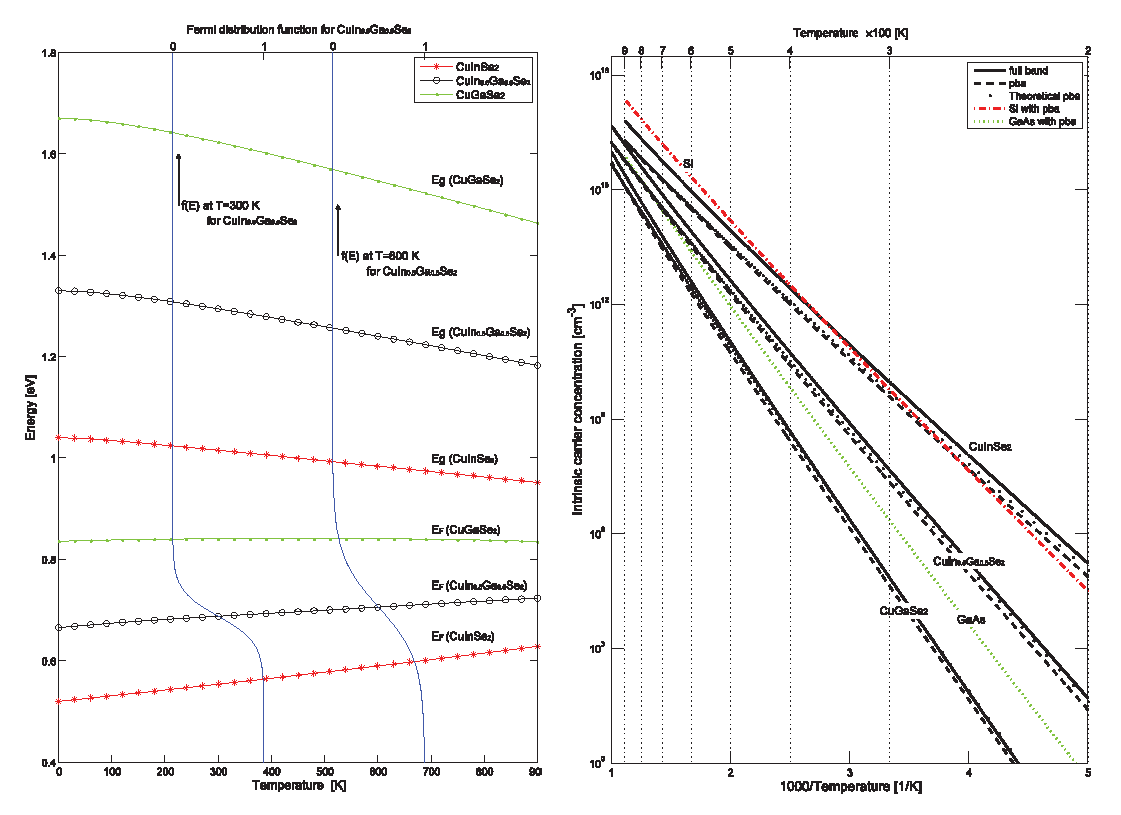
\includegraphics[width=1\textwidth,clip]{JAP4}
     \end{center}
    \caption{Left panel: Band-gap energy $E_g$ and Fermi energy $E_F$ for $1 \leq T \leq 900$ K of intrinsic CuInSe\textsubscript{2}, CuIn\textsubscript{0.5}Ga\textsubscript{0.5}Se\textsubscript{2}, and CuGaSe\textsubscript{2},
    determined from the fbp. In this figure, we also present the Fermi distribution $f(E)$ of CuIn\textsubscript{0.5}Ga\textsubscript{0.5}Se\textsubscript{2} for T = 300 K and 600 K. Right panel: 
    Intrinsic carrier concentration as function of temperature. For comparison, the theoretical results for GaAs and Si using the pba are given.}
   \label{icc}
\end{figure}


In \textbf{Fig. \ref{icc}}, the temperature dependent band-gap and Fermi level (left panel) and intrinsic carrier concentration (right panel) are shown.  In the left panel of \textbf{Fig. \ref{icc}}, the band-gap is 1.04, 1.33,
and 1.67 eV for the CuIn{\textsubscript{1-$x$}}Ga{\textsubscript{$x$}}Se\textsubscript{2}
where $x$ = 0, 0.5, and 1 at temperature around 0 K, respectively. Fermi level is exactly the mid-gap energy. The Fermi level changes only slightly with temperature. However, 
for CuInSe\textsubscript{2} and CuIn\textsubscript{0.5}Ga\textsubscript{0.5}Se\textsubscript{2}, the Fermi levels increase somewhat more compared with CuGaSe\textsubscript{2}. This is primarily because the CB of DOS mass for 
CuGaSe\textsubscript{2} is almost the same, but the VB of DOS mass for CuGaSe\textsubscript{2} change smaller compared with CuInSe\textsubscript{2} and CuIn\textsubscript{0.5}Ga\textsubscript{0.5}Se\textsubscript{2} which will 
affect the DOS. As a consequence, the Fermi level is closer to the CB minimum in the In rich compounds. At T = 300 K and 600 K, the band-gap energies $E_g$ and Fermi energy $E_F$ are given in \textbf{Table \ref{chen3}}

\begin{table}[H]
\centering
 \captionsetup{width=1\textwidth}
\scalebox{1}{
 \begin{tabular}{l c c c}
\hline
\cline{1-4}
  & CuInSe\textsubscript{2} & CuIn\textsubscript{0.5}Ga\textsubscript{0.5}Se\textsubscript{2} & CuGaSe\textsubscript{2} \\
\hline\hline
$E_g$ 300 K   [eV] &1.02  &1.29	&1.62	   \\
$E_g$ 600 K   [eV] &0.98  &1.24	&1.55	   \\
$E_F$ 300 K   [eV] &0.55  &0.69	&0.84      \\
$E_F$ 600 K   [eV] &0.59  &0.71	&0.84     \\
\hline
\end{tabular}}
\caption {Band-gap energies $E_g$ and Fermi energy $E_F$ at 300 K and 600 K, respectively.}\label{chen3}
\end{table}



In the left panel of \textbf{Fig. \ref{icc}}, the Fermi distribution of CuIn\textsubscript{0.5}Ga\textsubscript{0.5}Se\textsubscript{2} is given at 300 K and 600 K, respectively. The probability of occupying the VBM (CBM) by a hole (an electron) is 
relative increase of around $10^6$ times from 300 K to 600 K. In the right panel of \textbf{Fig. \ref{icc}}, the intrinsic carrier concentration is increased dramatically with the increasing of temperature for
the CuIn{\textsubscript{1-$x$}}Ga{\textsubscript{$x$}}Se\textsubscript{2} where $x$ = 0, 0.5, and 1. For example, in the case of CuInSe\textsubscript{2}, 
the carrier concentration is increased up to around $10^{5}$ times higher from temperature 300 K to 600 K. The intrinsic carrier concentration for the Si and CuInSe\textsubscript{2} are rather comparable. The free carrier 
concentration is increased goes up to 2$-$3 times by taking into account the non-parabolicity of the energy bands.

Since as-grown CIGS typically has $p$-type character, the Fermi level and $p$-type carrier concentration of free holes $n_v(T)$ and free electrons $n_c(T)$ are calculated by 
assuming the presences of the native Cu vacancies as acceptors. 

 \begin{figure}[H]
    \begin{center}
            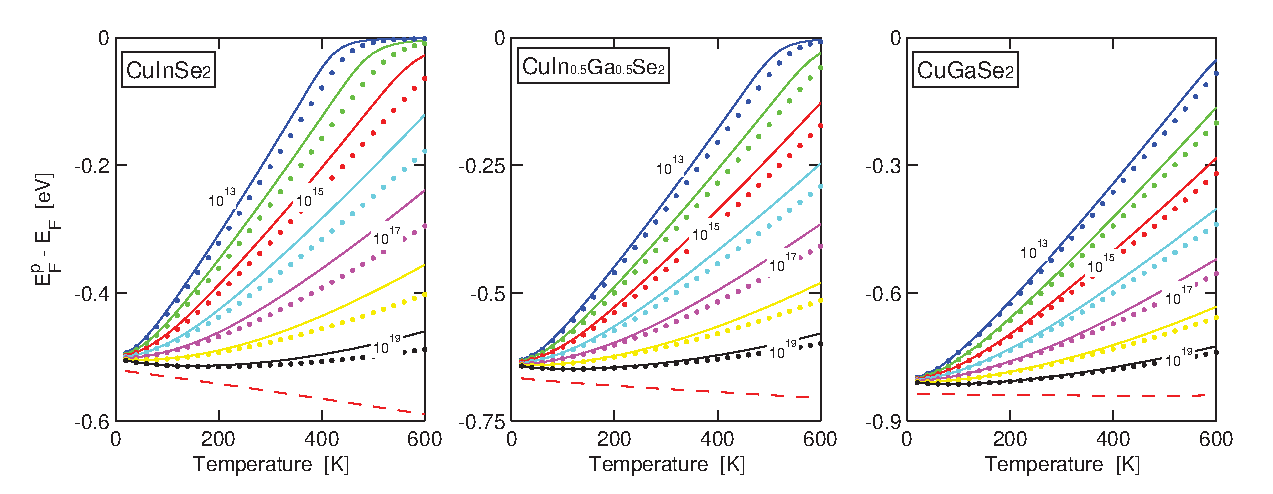
\includegraphics[width=1\textwidth,clip]{paper2fig81}
     \end{center}
    \caption{Fermi level as function of the temperature $20 \leq T \leq 600$ of $p$-type CuInSe\textsubscript{2}, CuIn\textsubscript{0.5}Ga\textsubscript{0.5}Se\textsubscript{2}, and CuGaSe\textsubscript{2} for the effective
    doping concentration $N_A$ = $10^{13}$, $10^{14}$, $10^{15}$, $\cdot$, and $10^{19}$ acceptors cm\textsuperscript{$-$3}. The energy scale $E_F^p-E_F$ describes the Fermi energy with respect to the intrinsic $E_F$ (\textbf{Fig. \ref{icc}}).
    Dashed lines represent the VBM with respect to the intrinsic Fermi level. Solid and dotted lines represents the fbp and the pba, respectively.}
   \label{ptypecc1}
\end{figure}




The calculated Fermi level $E_F^P$ in $p$-type materials is presented in \textbf{Fig. \ref{ptypecc1}}, referred to the Fermi level of the intrinsic materials $E_F$ from \textbf{Fig. \ref{icc}}. Only at very high temperatures
( $T > 400 K$) and for low acceptor concentrations, the Fermi level of $p$-type CuIn{\textsubscript{1-$x$}}Ga{\textsubscript{$x$}}Se\textsubscript{2}
where $x$ = 0, 0.5, and 1 can reach the Fermi level of corresponding intrinsic compounds. Moreover, although the different compounds have comparable acceptor ionization
energies, the Ga rich alloy has lower relative Fermi level; this is a direct consequence of the larger band-gap of the Ga rich alloy. By comparing the calculations with the pba (dotted lines in \textbf{Fig. \ref{ptypecc1}} ) and 
the fba (solid lines) for each of the three CuIn{\textsubscript{1-$x$}}Ga{\textsubscript{$x$}}Se\textsubscript{2}
where $x$ = 0, 0.5, and 1 alloys. One notices that the Fermi level is similar for the two models only at low and at very high temperatures. In the mid-temperature region the difference is however apparent.





The $p$-type carrier concentration (\textbf{Fig. \ref{ptypecc}}) for {CuIn\textsubscript{1-\textit{x}}Ga\textsubscript{\textit{x}}Se\textsubscript{2}} ($x$ = 0, 0.5, and 1) is presented using \textbf{Eq. \ref{ecc}}

 \begin{figure}[H]
    \begin{center}
            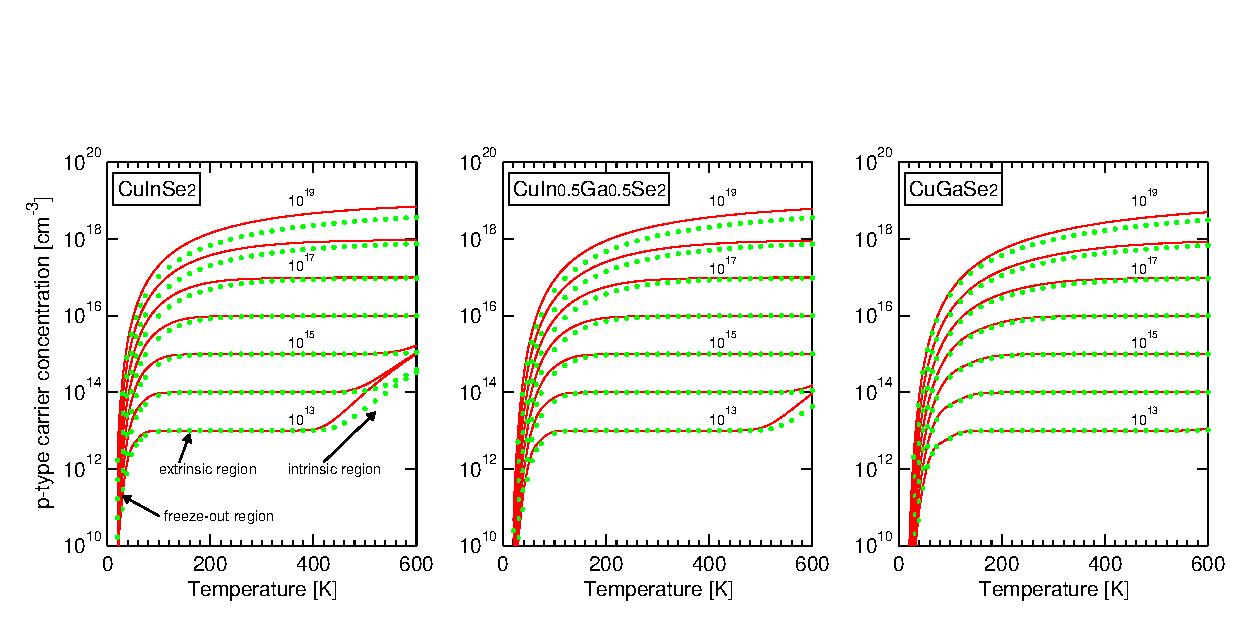
\includegraphics[width=1\textwidth,clip]{paper2figure9}
     \end{center}
    \caption{Free carrier concentration as function of the temperature in $p$-type for $\mathrm{CuInSe_2}$, $\mathrm{CuIn_{0.5}Ga_{0.5}Se_2}$, and $\mathrm{CuGaSe_2}$.
    The effective doping concentration $N_A = 10^{13}, 10^{14}, 10^{15}$,..., and  $10^{19}$ acceptors cm\textsuperscript{$-$3} are considered.}
   \label{ptypecc}
\end{figure}

In \textbf{Fig. \ref{ptypecc}}, the carrier concentration is recognized by three different regions: the freeze-out region, the extrinsic region and the intrinsic region. The 
transition from the freeze-out region to the extrinsic region happens below the room temperature except that the uncompensated acceptor concentration is above around 
$10^{18}$ cm\textsuperscript{$-$3}. The transition from the extrinsic region to the intrinsic region for In rich compounds occurs at the lower temperature since they have smaller band gaps.
The result based on the pba underestimates the carrier concentration around by the factor of 2 in the both freeze-out and intrinsic regions. Therefore, the 
non-parabolic energy bands is required in order to describe the carrier concentration more accurately.


\section{Dielectric function for CuIn\textsubscript{0.5}Ga\textsubscript{0.5}Se\textsubscript{2}}
The dielectric function ($\varepsilon (\omega)$ = $\varepsilon_1 (\omega)$ + i$\varepsilon_2 (\omega)$) spectra of CuIn\textsubscript{0.5}Ga\textsubscript{0.5}Se\textsubscript{2} is calculated by the all electron
and full-potential linearized augmented plane wave (FPLAPW) method. The calculated dielectric function is compared with experimental values (CuIn\textsubscript{0.7}Ga\textsubscript{0.3}Se\textsubscript{2}) at temperature 
of 40 K and 300 K. They are in a good agreement. The different contributions to $\varepsilon_2(\omega)$ in terms of the transitions between the valence bands and the conduction bands are identified based on this calculation.
Moreover, the $\textbf{k}$-dependence of the interband critical points (CPs) along the main symmetry directions is analyzed as well.

 \begin{figure}[H]
    \begin{center}
            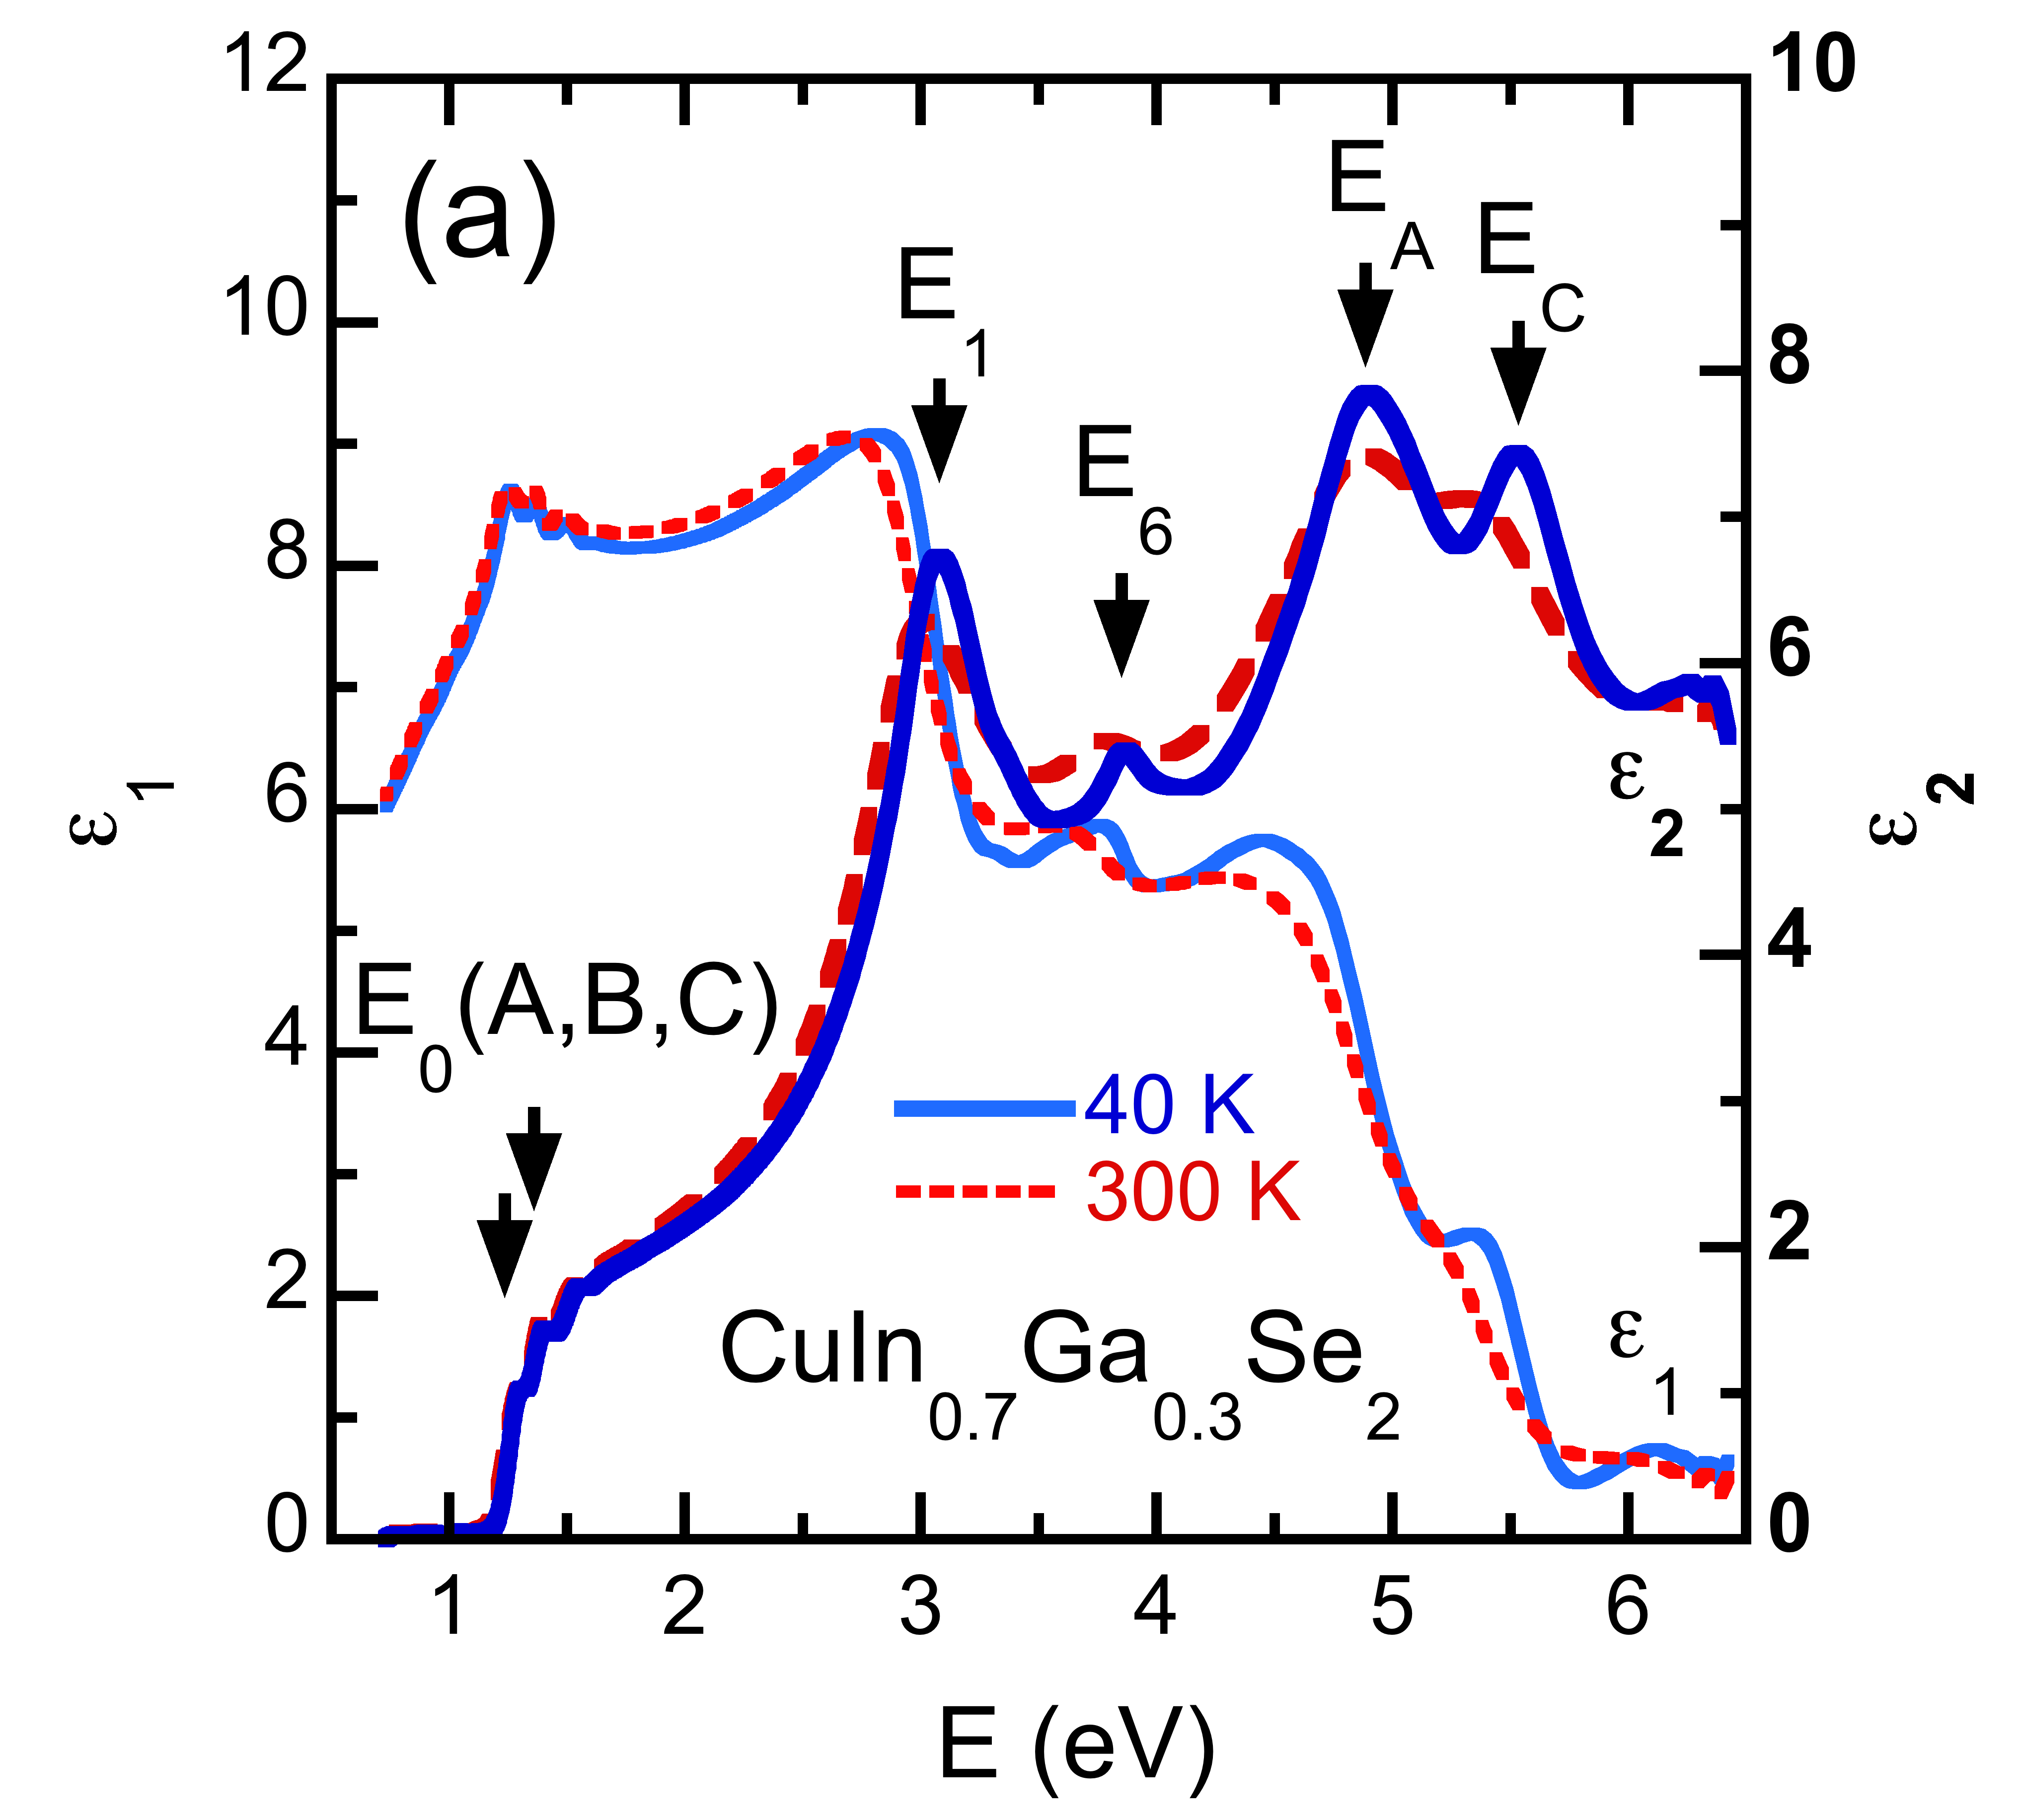
\includegraphics[width=0.5\textwidth]{APL1b.jpg}
            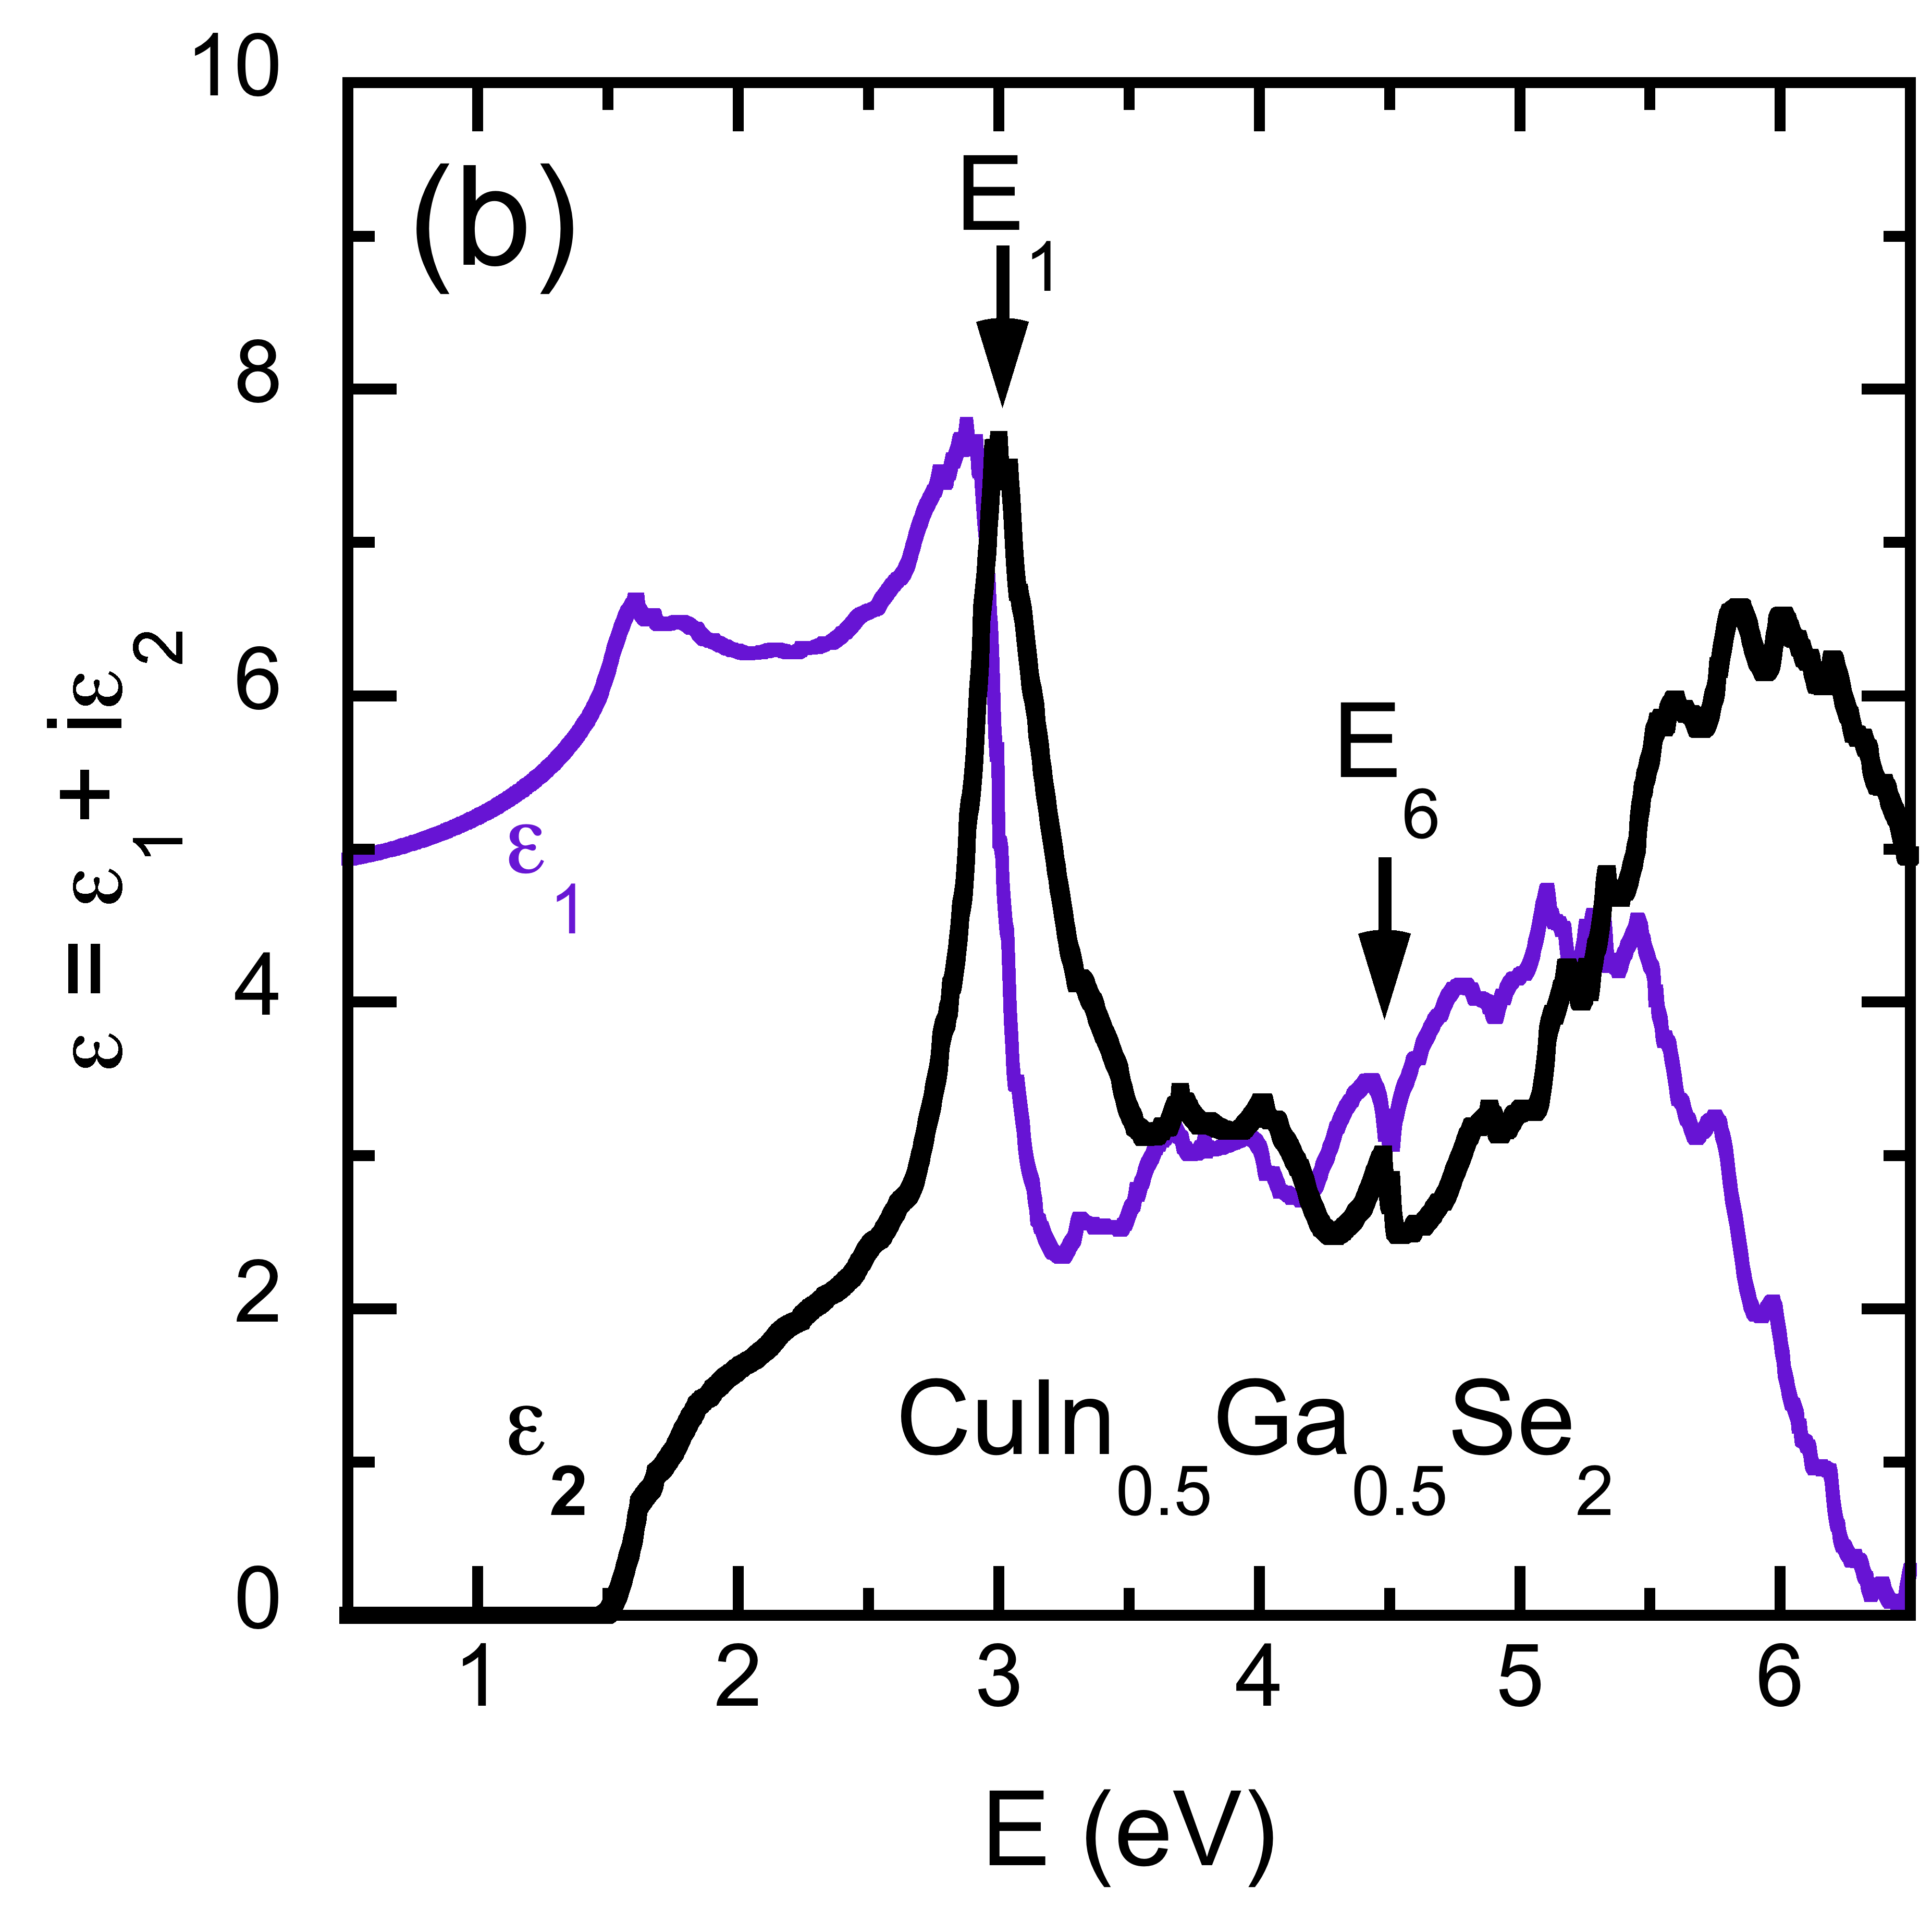
\includegraphics[width=0.45\textwidth]{APL1a.jpg}
     \end{center}
    \caption{Left panel: The real ($\varepsilon_1$) and imaginary ($\varepsilon_2$) part of dielectric function spectra for CuIn\textsubscript{0.7}Ga\textsubscript{0.3}Se\textsubscript{2} 
at 40 K (solid blue line) and 300 K (dashed red lines). Four prominent CP features are shown. Right panel: the dielectric function spectra for CuIn\textsubscript{0.5}Ga\textsubscript{0.5}Se\textsubscript{2}
calculated by FPLAPW method at 0 K. The major CP features are identified. }
   \label{df1}
\end{figure}

In \textbf{Fig. \ref{df1}}, the general shape between experimental and calculated dielectric function is relatively similar. The calculation indicates that there is no big difference in the optical properties for those 
two materials, except the shift of CP energies. The analysis based on experimental work indicates that there are twelve CPs from 2.5 eV to 6.4 eV. Therefore, the electronic origin for each CP is analyzed based on 
the calculated results. The contribution to dielectric function between the valence bands and conduction bands is presented as well in \textbf{Fig. \ref{df2}}.


 \begin{figure}[H]
    \begin{center}
            \includegraphics[width=0.75\textwidth]{APL34}
     \end{center}
    \caption{Upper panel: band-to-band analysis of the contribution to the total $\varepsilon_2$ spectrum. The vertical axis is in the log scale. 
              lower panel: the calculated electronic band structure of CuIn\textsubscript{0.5}Ga\textsubscript{0.5}Se\textsubscript{2} where the CPs are identified along the main symmetry directions.}
   \label{df2}
\end{figure}

Here, $v_1$ and $c_1$ represent the topmost valence band and lowest conduction band, respectively. From \textbf{Fig. \ref{df2}}, one notices that the $E_1$ CP comes from 
the $v_1 \longrightarrow c_1$ transition near the P(1/2, 1/2, 1/2) point of the Brillouin zone (BZ). The $E_2$ and $E_3$ CPs are corresponding to transition of $v_2 \longrightarrow c_1$ in the P point
as well in the BZ. The $E_2$ and $E_3$ CPs are small peak in the \textbf{Fig. \ref{df2}}. However, the calculation of CuInSe\textsubscript{2} indicates that they happens 0.1$-$0.2 eV higher than 
the $E_1$ CP, which is distinct spectral features (\textbf{Fig. \ref{ccccc}}). The $E_4$ CP comes from the transition of $v_3 \longrightarrow c_1$ at the $M (1,0,0) = M^*(0,0,1)$ point.
The $E_5$ CP is contributed by the transitions $v_4 \longrightarrow c_1$ at the $N (1/2,0,1/2)$ point and $v_3 \longrightarrow c_1$ at the $M/M^*$ point. The $E_6$ CP feature
corresponding to the  $v_4 \longrightarrow c_1$ at the $N$ point. The $E_7$ is from the transitions $v_4 \longrightarrow c_2$ at the $\Gamma (0,0,0)$ and N point, the 
  $v_5 \longrightarrow c_2$ at the $\Gamma$ point is also contributed.


\begin{figure}[H]
\begin{center}
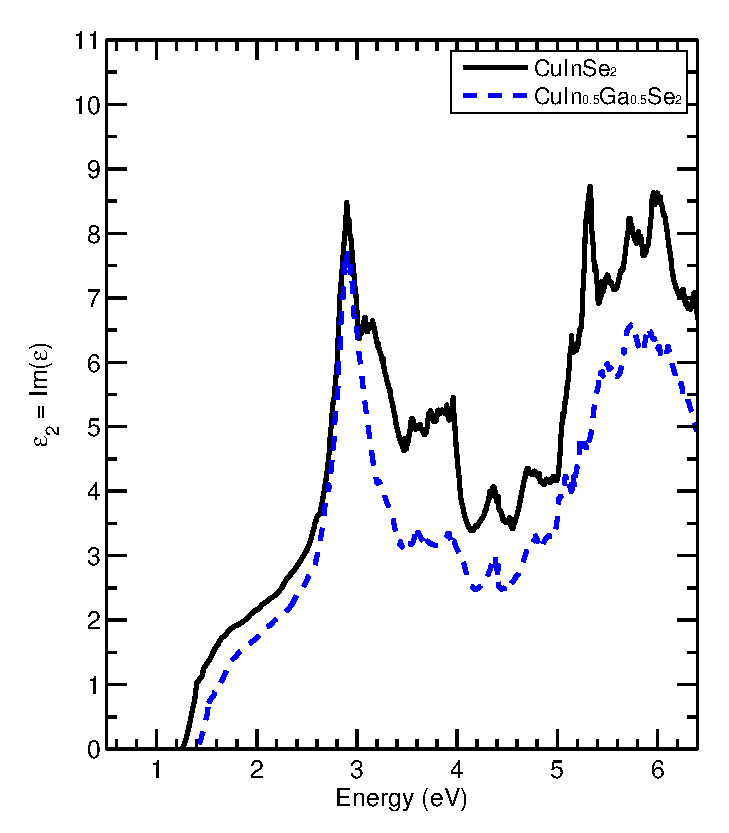
\includegraphics[scale=0.5]{thesis2.eps}
\end{center}
\caption{The $\varepsilon_2$ spectra for CuInSe\textsubscript{2} and CuIn\textsubscript{0.5}Ga\textsubscript{0.5}Se\textsubscript{2}. }
\label{ccccc}
\end{figure}

\end{comment}


\chapter{SHORT SUMMARY OF THE PAPERS}

\section{Summary of the papers}

I \textbf{Parameterization of $\mathbf {CuIn_{1-x}Ga_{x}Se_2}$ (x = 0, 0.5, and 1) energy bands}
\\\textbf{R. Chen} and C. Persson, \textit{Thin Solid Films} {\textbf {519}}, 7503 (2011).

The most fundamental property of a material is the energy of the electrons. That is determined by solving the Kohn-Sham equation (see \textbf{Eq. \ref{aaa111}}). By understanding the electronic properties of the electrons one 
can understand many of the fundamental material properties. During the last two decades the electronic structure of CIGS has been explored, however the motivation of the present study is that much of the earlier studies describe 
the electronic structure and the corresponding density-of-states (DOS) on a wider energy scale, typically from 5$-$10 eV below valence bands maximum (VBM) to 5$-$10 eV above conduction band minimum (CBM). With that perspective one
gets the overall understanding of the material, and one also gets the bond character, but details near the band edges are less revealed. The reason why details are important can be understood from different energy of relevance in
materials. The energy to create defects is typically on the eV-scale (a Cu vacancy costs about 0.8 eV to be formed in CIS), the energy of band filling in heavily doped, degenerated semiconductors are typically in the 0.1 eV scale, and
room temperature corresponds to $k_BT $ (around 0.025 eV). Thus, to understand band filling and transport of electrons/holes one has to understand the electronic structure on an energy scale of 1 meV to around 0.1 eV. Moreover, most of the
earlier studies are on the ternary compounds CIS and CGS, whereas the experimentally and commercially most interesting compound is the CIGS alloy with about 70\% In and 30\% Ga, that is
Cu\textsubscript{2}In\textsubscript{0.7}Ga\textsubscript{0.3}Se\textsubscript{2}. It is therefore interesting to understand how Ga-on-In alloying affects the electronic structure.   

In this paper, we have therefore conducted a study on CuIn\textsubscript{1-\textit{x}}Ga\textsubscript{\textit{x}}Se\textsubscript{2}, with $x$ = 0, 0.5, and 1. Here, $x$ = 0.5 is not exactly the same configuration as for the
commercially interesting compound, but it indicates how CIGS behaves when alloying In and Ga. Moreover, the present study focuses on the details in the electronic structure near the band edges. We do that by analyzing
the lowest conduction band (CB) and the three uppermost valence bands (VBs) of CIGS ($x$ = 0, 0.5, and 1) based on the FPLAPW calculations (Section \ref{fplapwm}) of the electronic band structure. The advantage of using the FPLAPW within the 
Wien2k package is that the code generates very accurate energy values in terms of noise and level of degeneracy of states, while the disadvantage is that the code does not have same possibility of choosing post-DFT calculations.
Having accurate description of the degenerate states at $\Gamma$-point VBM is crucial when determining the effective hole masses there since one needs an accuracy of 0.01$-$0.1 meV. Therefore, we follow the FPLAPW calculation approach
described in Ref. \cite{persson2008anisotropic} which has shown to be able to overcome the problem with unwanted interaction between VB and CB states which can strongly affect the values of effective masses. It has also been proven
to generate accurate values of the effective masses Ref. \cite{persson1997relativistic}, and our result for effective electron mass of CIS ($m_{c1}$=$0.08m_0$) is close the experimental results ($m_{c1}$=$0.09m_0$)
by Weinert \cite{neumann1978electrical}. Thus, even if we do not generate the band structure with the exact exchange-correlation potential, we have reason to believe that the results are fairly good, and the results are useful when 
analyzing future measurements and simulations.

In this paper we present parameterization of electronic band structure of the lowest CB and the three uppermost VBs. These bands are the most important bands for electron and hole transport in the material. With the parameterization
of the bands, other researchers can easily generate the energy bands in order to further investigate properties that are related to band filling and carrier transport. 

The parameterization of the energy bands demonstrates that the energy dispersions of the lowest CB and three uppermost VBs are strongly anisotropic and non-parabolic close to the $\Gamma$-point. This anisotropy and non-parabolicity 
directly affect the effective electron and hole masses. Thereby we can better understand the CIGS. This parameterization method can be utilized to other materials potentially, such as kesterite and stannite 
Cu\textsubscript{2}ZnSn(S,Se)\textsubscript{4}, which we have presented in another work \cite{X}.

Using the parameterized electronic structure, we analyze the electrons and holes effective masses for these bands. 
The effective mass tensor ($\pm \hbar / (\partial^2E(\mathbf{k})/\partial{\mathbf{k}^2}) $) is directly related to the curvature of the bands. The effective mass of the electron (or hole) is a very fundamental property of
semiconductors and is used for various
analyses of experiments and carrier transport simulations. Low effective mass value normally means better transport of the carriers, this is very important for the minority carriers
(i. e., the electrons in $p$-type CIGS). In addition, and in models the effective mass is often used to approximately describe the band structure around the band edge, for instance to model band filling. Thus, the effective mass
is used in two ways: to describe transport of a single carrier and to describe collective band filling. The effective masses are normally presented (both experimentally and theoretically) as constant value at the very minimum
of the CBM or the very maximum of the VBM. That is correct if one can measure (or accurately calculate) details in the electronic structure near the band edges. However, very often one measures effective masses indirectly and for
a material with high electron and hole concentrations. Therefore the measured mass value is not the mass at the very CBM or VBM but the mass near the quasi Fermi level. We therefore describe the effective mass both
as the $\Gamma$-point effective mass of the CB and the three VBs, but also an average mass that is energy-dependent and shall better represent the effective mass in models that describe transport. That is, one can use the
energy-dependent mass $m(E)$ in existing models and a little better describe the physics of the material.      

In \textbf{Fig. 3} of Paper I, we illustrate how strongly the effective masses of the bands depend on specific \textbf{k}-state that one considers. The $\Gamma$-point effective mass (value when wave vector equals $\mathbf{0}$) 
is only valid close to the $\Gamma$-point. Already some 5$-$10\% away from the $\Gamma$-point mass value has changed. This is very obvious for the second uppermost VB (red lines) in CIS. One can notice that the behavior of
the effective electron masses are similar while it differs much more for the effective holes masses between of the three compounds (i.e., $x$ = 0, 0.5, and 1.0). 
This is a direct consequence of the different spin-orbit split-off and the crystal-field split-off energies. These splits directly affect the band curvatures and therefore the effective masses. This is discussed in the paper. Moreover, in the figure one can see that the effective mass is very anisotropic, that is, different 
in different $\mathbf{k}$ directions; this is most obvious for the holes in the VBs. That means that carrier transport will be different in different $\textbf{k}$ directions.  



II \textbf{Band-edge density-of-states and carrier concentrations in intrinsic and $p$-type
\\$\mathbf {CuIn_{1-x}Ga_{x}Se_2}$}
\\\textbf{R. Chen} and C. Persson, \textit{J. Appl. Phys.} {\textbf {112}}, 103708 (2012).

\noindent 
When a solar cell is under operation, the sunlight  strongly excites electrons up to the CB and
thereby also creating holes in the VBs. Then, one has quasi Fermi levels for the CB and the VBs.  
Also, with illumination, the device operation is in the order of 25 degrees Celsius and the temperature 
affects the carrier concentration. 
In addition, if the material is $n$- or $p$-type, one also needs to consider the electron states related 
to the dopants.    

The motivation of this study is that we utilize the parameterized band dispersion of 
CuIn\textsubscript{1-\textit{x}}Ga\textsubscript{\textit{x}}Se\textsubscript{2} ($x$ = 0, 0.5, and 1) 
in Paper I, and we want 
better analyze the impact on density-of-states (DOS) as well as carrier concentrations and Fermi energy
by taking into account the non-parabolicity and anisotropy of the energy bands. 

 
That is, in this work we explore how temperature and doping affect the carrier concentration and we compare the 
analyses done with  the true, full electronic band structure and done with a corresponding model 
of the band structure generated 
by the $\Gamma$-point effective mass; the latter model is commonly used in semiconductor physics. 
In the paper, we denote these two models as full band parameterization (fpb) and the parabolic band approximation (pba), respectively.  
Also here we analyze the ternaries CIS ($x$ = 0) and CGS ($x$ = 1), but also the CIGS alloy with $x$ = 0.5 to complement the analyses for materials that are used in today's solar cells. 
In the paper, we explore the DOS of the VBs and the CB, and we find that the parabolic approximation very poorly describes the DOS for especially the VB. Normally one uses the effective DOS mass to represent 
the parabolic description of the DOS, but that is thus not an accurate method for the VBs in CIGS. Therefore, we introduce energy-dependent DOS mass that can better represent the energy-dependent DOS, and that can 
be used in the traditional models. That is, with the DOS mass one can describe the band filling better, still using models that have been derived for a constant value of the DOS mass. The advantage is that the energy-dependent 
mass easily can be used in analyses of measurements where band filling is strong.

Moreover, with the parameterized bands we analyze temperature dependence of the carrier concentrations ($n$ = $p$) in intrinsic material. As expected, the carrier concentration depends much on the band-gap energy of the material; 
the carrier concentration for Si (multi-valley CBM and $E_g$ $\approx$ 1.2 eV) is similar as in CIS ($E_g$ $\approx$ 1.0 eV) and the carrier concentration for GaAs ($E_g$ $\approx$ 1.5) lies between CIGS with
$x$ = 0.5 ($E_g$ $\approx$ 1.3 eV) and CGS ($E_g$ $\approx$ 1.6 eV).       

We also model the temperature-dependent Fermi levels and carrier concentrations in $p$-type CIGS 
since the material is used as $p$-type absorber layer in solar cells. Thus, an accurate description of the temperature dependences are important in analyses and simulations of the material and devices. Here, we find that there 
is a large difference for the full band description compared with the parabolic approximation. The difference is explained by the non-parabolicity and anisotropy of the energy bands.  

\noindent In details, the overall results are: 
(i) the three uppermost valence bands (VBs) are strongly anisotropic and non-parabolic. (ii) The lowest CB becomes non-parabolic for energies 50$-$100 meV above the $\Gamma$-point band minimum. (iii) A constant
density-of-states (DOS) mass cannot accurately describe band filling of the valence bands even at low hole concentrations. Instead, we introduce an energy-dependent DOS mass that can be utilized to describe the carrier concentration 
and the Fermi energy using traditional equations for the DOS. (iv) With the full description of the energy dispersion, the hole concentration is improved by a factor of 10$-$50 and the electron concentration is improved by a factor
of 2$-$10 depending on quasi-Fermi energy. (v) The transition from the freeze-out region to the extrinsic region occurs well below the room temperature for uncompensated acceptor concentration below 
around 10\textsuperscript{17} cm\textsuperscript{$-$3}, whereas for higher concentrations, not all acceptors are ionized at T = 300 K. Thus, with a more correct description of the energy dispersions, one can better analyze the
electron and hole dynamics in the CuIn\textsubscript{1-\textit{x}}Ga\textsubscript{\textit{x}}Se\textsubscript{2} ($x$ = 0, 0.5, and 1) alloys, thereby better understand the electrical properties of these compounds. 

III \textbf{Dielectric function spectra at 40 K and critical-point energies for $\mathbf {CuIn_{0.7}Ga_{0.3}Se_2}$}
S.G. Choi, \textbf{R. Chen}, C. Persson, T.J. Kim, S.Y. Hwang, Y. D. Kim, and L. M. Mansfield,
\textit{Appl. Phys. Lett. } {\textbf {101}}, 261903 (2012).

The most important optical property of a solar cell material is how the material absorbs the sunlight efficiently. The absorption coefficient $\alpha(\omega)$ describes this efficiency in units of 1/length.
That is, if the absorption coefficient is large, the thickness of the material can be thinner but still the material absorbs the same amount of sunlight. The absorption coefficient is related to the dielectric function through
the expression in \textbf{Eq. \ref{czr852}}. There the imaginary part $\varepsilon_2(\omega)$ of the dielectric function is closely related to the absorption coefficient; for instance, 
both $\varepsilon_2(\omega)$ and $\alpha(\omega)$ are zero for photon energies smaller than the band-gap.  That is, by analyzing the dielectric function one can also understand how the optical transition occurs and
how good or bad the material is for a solar cell. That is, the imaginary part of the dielectric function is obtained from 

\begin{equation}
\varepsilon_2^{\alpha\beta} (\omega)= \frac{\hbar e^2}{\pi m^2\omega^2} \sum_{cv} \int d \textbf {k} <\Psi_{c{\textbf k}}|p^\alpha|\Psi_{v{\textbf k}}><\Psi_{v{\textbf k}}|p^\beta|\Psi_{c{\textbf k}}> (f(\varepsilon_{c \textbf k})-f(\varepsilon_{v \textbf k}))\delta(\varepsilon_{c {\textbf k}}-\varepsilon_{c{\textbf k}}-\omega).
\end{equation}

Thus, it is a summation of all possible band-to-band direct transitions from unoccupied to occupied states. The energy needed for excitation depends on the energy difference between final and initial states (indicated by the 
delta-Dirac function in the equation) and the strength of the absorption possibility which is described by the 
optical matrix element $<\Psi_{c{\textbf k}}|p^i|\Psi_{v{\textbf k}}>$. While the energy difference between final and initial states only depends on the electronic band structure, the optical matrix element depends
on the shape and symmetry of the electron wave function. Certain band-to-band transition can be weak or strong depending on the wavefunction of the final and initial states. To understand the optical properties of a material, 
one needs to analyze the dielectric function in details.  

 
\noindent The motivation of this study is that we help experimentalists to understand the dielectric function spectrum 
of CuIn\textsubscript{0.7}Ga\textsubscript{0.3}Se\textsubscript{2}, but we also want to understand details in the optical transition for these types of materials. That is, we want to explore which energy bands and which electrons states are 
most optical active when the solar cell is under operation. 
By understanding that we can better explain the optical activity of the CIGS material, but also understand how one shall modify the material or tailor-make similar compounds with even better optical efficiency.   


\noindent In this paper, we have therefore calculated the spectrum of the dielectric function for CuIn\textsubscript{0.5}Ga\textsubscript{0.5}Se\textsubscript{2} by means of the all-electron FPLAPW method as in Papers I and II. 
The calculated dielectric function is compared with experimental data (CuIn\textsubscript{0.7}Ga\textsubscript{0.3}Se\textsubscript{2}) at temperatures of 40 K and 300 K, and we find that results based on theory and experiment are in reasonable good agreement. We decompose the full dielectric funcition into the contributions from each band-to-band transition and for each state in the Brillouin zone.  The different contributions to imaginary part of dielectric function in terms of the transitions between the valence bands and the conduction bands are identified based on this
calculation. Moreover, the $\textbf{k}$-dependence of the interband critical points along the main symmetry directions are analyzed as well. With these results, we can better understand and explain the dielectric function spectra obtained
by experimentalist. The surprising conclusion is that there are different band-to-band transitions that are important and that several low-lying states in the VBs that strongly contribute to the total dielectric function. That is, a full band description is needed to accurately describe the optical activity of these materials.




\section{Concluding remarks and future perspectives}

\noindent Chalcopyrite CIGS is seen as one of the most promising materials for the near future 
thin-film solar-cell technology. The maximum conversion efficiency of 23.3\% for the CIGS was achieved in the 
laboratory \cite{ward2014cu}. Solar cell modules based on CIGS are already commercially reality and contribute today with 
about 2.5\% of the solar cell market.
 
Although the material properties are known from earlier theoretical and experimental 
studies, details in the electronic structure of the band edges are less studies, especially not for the alloy CuIn{\textsubscript{1-$x$}}Ga{\textsubscript{$x$}}Se\textsubscript{2} .

In this licentiate thesis, two major researches are presented: (i) Analysis of the electronic structure 
of CuIn{\textsubscript{1-$x$}}Ga{\textsubscript{$x$}}Se\textsubscript{2} with $x$ = 0, 0.5, and 1. 
Here, we parameterize the energy bands in order to better describe energy dispersions and better analyze 
the electron and hole dynamics in the materials. We consider intrinsic and $p$-type  materials, and we model
the temperature dependence. The research is presented in Paper I and II.
(ii) Analysis of the optical properties of CuIn{\textsubscript{0.5}}Ga{\textsubscript{0.5}}Se\textsubscript{2}. 
Here, the dielectric function spectra is calculated and compared with experimental result. 
The probable electronic origins of the critical point features are discussed as well.
The research is presented in Paper III.


Overall, we find that it is important to consider the full band description of the material to understand the
fundamental properties of the electronic structure and the optical activity. Especially, the energetically high
lying Cu $d$-states in CIGS plays a significant role since they hybridized with the In or Ga and Se states near the VBM and some 2$-$5 eV below the VBM.  Cu $d$-states form flat energy bands in the VB that contribute to a
high optical efficiency of the compound. This hybridization makes the VBs very non-parabolic, also for the uppermost VBs at least away from the $\Gamma$-point of the Brillouin zone. Therefore, a parameterization of the bands is
rather complex. Moreover, we find that it is crucial to include the spin-orbit interaction when analyzing details in the electronic structure. Both the spin-orbit split-off and the crystal-field split-off make the uppermost VBs
strongly non-parabolic also close to the $\Gamma$-point. The impacts of the spin-orbit interaction and the crystal-field are less important when studying properties related to total energy, like ion relaxation, defect formation 
energies, etc, but in studies related to excitation, band filling, and carrier transport one needs to consider these effects.        


\noindent 
For future perspective and from a theoretical point of view, improved analyses can be done when better computational methods are developed. The LDA and GGA are fairly accurate methods, but have limitations 
in terms of inaccurate band-gap energies and localization of $d$- and $f$-states. The GW approach that we employ today is very time-consuming and it does not generate total energies; that limits the usability of the approach. 
Hybrid functionals (like HSE \cite{paier2006screened}) can give better band-gap energies, but this approach is as time-consuming as the GW approach which is a limitation for extensive research of complex materials. Moreover, there are discussions how
the approach is to model details in accurately for instance defect transition energies. 
That is, further development of computational methods will help improving the results, however it is not certain that
it will reveal very much new physics. Already with LDA and GGA we have reasonable understanding of the materials.    

By understanding the electronic and optical properties of CIGS, we have the basic knowledge for studying also 
alternative materials in the future. Ideally, such materials should consist of inexpensive, earth-abundant, 
and non-toxic elements in addition to have crystal stability and high optical absorption efficiency.  

The cost and scarcity of indium in the CIGS device is a problem, and  copper zinc tin selenide 
(Cu\textsubscript{2}ZnSnSe\textsubscript{4}) and
copper zinc tin sulfide (Cu\textsubscript{2}ZnSnS\textsubscript{4}) 
can therefore be alternative to CIGS due to the low cost and non-toxicity elements. 
Cu\textsubscript{2}ZnSn(S,Se)\textsubscript{4} has many similarities with CIGS, such as comparable crystal structure and 
tunable band-gap via anion alloying, as well as similar solar cell device structure and fabrication techniques. 
Since the research on those materials is relatively young, the solar-cell conversion efficiency
is only around 12.6\% in the laboratory \cite{wang2014device}. The disadvantage is however that  these quaternary 
chalcogenide semiconductors are more complicated compared with the more traditional thin-film materials, 
and the materials have more complex native defects. 

One can also speculate if there are other similar materials that are of interest. CIGS and CZTS can be 
considered to be in a class denoted as Cu-XY-chalcogenide, where X and Y are two cation elements that replace the 
group-III In or Ga in CIGS. From the present study, we understand the advantage of having Cu as an element in the 
compound, but with choosing proper element for additional cation element one can maybe find optimal material 
with higher absorption coefficient.  
For instance, there are interesting papers describing Cu(Sb,Bi)(S,Se)\textsubscript{2} indicating very high absorption coefficient. 
Of course, Sb or Bi is not the best element to replace In or Ga, but by understanding the electronic and optical 
properties of these materials one can further understand the Cu-XY-chalcogenide type compounds.    
Cu\textsubscript{2}O is studied as an absorber material for solar cells quite earlier \cite{RevModPhys5141}, and this material is still considered as an interesting solar cell material if one can stabilize the structure.
Cu\textsubscript{2}S or Cu\textsubscript{2}(O,S) is an alternative to that type of material.

For all these materials, and perhaps other Cu-XY-chalcogenide compounds one needs to explore the electronic and optical properties in combination with studies of crystalline stability/degradation, defect formation, and dopability. 
By systematically analyzing and understanding the materials one has better possibilities to tailor-make compounds with optimal performance for thin-film, and perhaps ultra-thin-film solar cells.


 

\begin{comment}
\chapter{Appendices}

In order to solve the Hartree, Hartree-Fock and Kohn-Sham equation, some mathematical knowledge need to be introduced in this section, that is, Lagrange multiplier and functionals.

\textbf{Lagrange multiplier}

Lagrange multiplier is a method which can maximize or minimize functions with the constraint. In order to maximize or minimize a function $f(x,y,z)$ with constraint $g(x,y,z) = c$,  the generalized format of Lagrange multiplier
method is given as

\begin{equation}
\begin{split}
& \frac{\partial \left( f(x,y,z) - \lambda g(x,y,z)\right)}{\partial x} = 0 \\
& \frac{\partial \left( f(x,y,z) - \lambda g(x,y,z)\right)}{\partial y} = 0 \\
& \frac{\partial \left( f(x,y,z) - \lambda g(x,y,z)\right)}{\partial z} = 0 \\
& \frac{\partial \left( f(x,y,z) - \lambda g(x,y,z)\right)}{\partial \lambda} = 0.
\end{split}
\end{equation}


For example, assume that the ground state wavefunction is $\Psi_0$, and ground state total energy $E_0$ is give as

\begin{equation}
 E_0 = \min(E) = \min<\Psi (\textbf{r}) | \widehat{H} | \Psi (\textbf{r})>, \mathrm{and} \  \Psi(\textbf{r}) \longrightarrow \Psi_0(\textbf{0}).
\end{equation}

The constraint of wavefunction is normalization
\begin{equation}
 <\Psi(\textbf{r}) |  \Psi(\textbf{r})> = 1.
\end{equation}

Therefore, problem of the ground state total energy can be solved by Lagrange multiplier method
\begin{equation}\label{lagmul}
\begin{split}
&  \frac{\partial \left( E - \lambda g \right)}{\partial \Psi(\textbf{r})} = \frac{\partial \left( <\Psi (\textbf{r}) | \widehat{H} | \Psi (\textbf{r})> - \lambda (<\Psi(\textbf{r})|\Psi(\textbf{r})>-1) \right)}{\partial \Psi(\textbf{r})} = 0, \\
&  \frac{\partial \left( E - \lambda g \right)}{\partial \lambda} = \frac{\partial \left( <\Psi (\textbf{r}) | \widehat{H} | \Psi (\textbf{r})> - \lambda (<\Psi(\textbf{r})|\Psi(\textbf{r})>-1) \right)}{\partial \lambda} = 0.
\end{split}
\end{equation}

\textbf{Functional}

A functional takes a function as an input, and output is a number. In previous section, the total energy $E$ is the function of wavefunction $\Psi(\textbf{r})$, which is a functional. In order to solve the \textbf{Eq. \ref{lagmul}}, 
basic properties of functionals and their derivatives are needed to introduced.

Assume that a set of points are defined as $y^0 = (y_1^0, y_2^0, \cdots, y_N^0)$. A function with multivariables is given as $F(y_1, y_2, \cdots, y_N)$, then a small change away from $y^0$ leads to the change of
function $F(y_1, y_2, \cdots, y_N)$ by 

\begin{equation}\label{functional1}
\delta F(y_1, y_2, \cdots, y_N) = \sum\limits_{i=1}^N \frac{\partial F(y_1, y_2, \cdots, y_N)}{\partial y_i} {\Big |}_{y_i^0}  \delta {y_i}.
\end{equation}

A one-to-one map $y_n = g(x_n)$ is defined where $g(x_n)$ has $N$ finite number of variables. In order to be utilized in physics, the $g(x_n)$ can be allowed all the real numbers in certain interval, such as $[x_0, x_N]$, that is,
$N$ is allowed to be infinite number ($\infty$). 

Assume that $x_n$ is defined within interval $[x_0, x_N]$, and there are $N$ points in this interval, as well as $x_{n+1}-x_{n} = \varepsilon$. Therefore, $x_N-x_0 = N \varepsilon$, that is, $x_n = n \varepsilon + x_0$, 
and $y_n = g(x_n) = g (x_0+n \varepsilon)$. Therefore, $g(x_n) = g(x)$ with the limit $\varepsilon \rightarrow 0$ and $N \rightarrow \infty$,  where $x$ can be any real number in the interval. That is, $F(g(x_1), g(x_2), \cdots, g(x_N))
= F(g(x))$ under the limit of $N \rightarrow \infty$, which is a functional.

The derivative of function can lead to the derivative of functionals. If the $y_n$ is substituted for $g(x_n)$ in \textbf{Eq. \ref{functional1}}, the new equation is given as


\begin{equation}\label{functional2}
\delta F(g(x_1), g(x_2), \cdots, g(x_N)) = \sum\limits_{i = 1}^N \frac{\partial F(g(x_1), g(x_2), \cdots, g(x_N))}{\partial g(x_i)} {\Big |}_{g^0(x_i)}  \delta {g(x_i)}.
\end{equation}


Recall the definition of integral for function

\begin{equation}
 \int_{x0}^{x_N} f(x)dx = \lim\limits_{\varepsilon_{i} \rightarrow 0} \sum\limits_{i = 1}^{N} \varepsilon_{i}f(x_i), \mathrm{where}\ N \rightarrow  \infty.
\end{equation}


Therefore, the \textbf{Eq. \ref{functional2}} is equivalence to

\begin{equation}\begin{split}
& \delta F(g(x_1), g(x_2), \cdots, g(x_N)) \\
& = \sum\limits_{i = 1}^N \frac{\partial F(g(x_1), g(x_2), \cdots, g(x_N))}{\partial g(x_i)} {\Big |}_{g^0(x_i)}  \delta {g(x_i)} \\
& = \sum\limits_{i = 1}^N \varepsilon_i \frac{\partial F(g(x_1), g(x_2), \cdots, g(x_N))}{\varepsilon_i \partial g(x_i)} {\Big |}_{g^0(x_i)}  \delta {g(x_i)} \\
& =  \int_{x0}^{x_N} \frac{\partial F(g(x))}{\partial g(x)} {\Big |}_{g^0(x)} \delta g(x) dx \\
& = \int \frac{\partial F(g(x))}{\partial g(x)} \delta g(x) dx \\
& = F[g(x) + \delta g(x)] - F[g(x)]
\end{split}
\end{equation}

In order to calculate the derivative of a functional in reality, first, $F[g(x) + \delta g(x)] - F[g(x)]$ is solved using Taylor expansion; 
Second, the result from first step is compared with $\int \frac{\partial F(g(x))}{\partial g(x)} \delta g(x) dx $. For example, a functional $F[g(x)] = \int f(g(x)) dx$  is defined, and  

\begin{equation}
\begin{split}
& F[g(x) + \delta g(x)] - F[g(x)] \\
& = \int f(g(x)+\delta g(x)) dy - \int f(g(x))dy \\
& = \int ( f(g(x))+ \frac{\partial f(g(x))}{\partial g(x)} \delta g(x) + O(\delta g(x))^2)dx - \int f(g(x))dx \\
& = \int \frac{\partial f(g(x))}{\partial g(x)} \delta g(x) dx
\end{split}
\end{equation}

Therefore, 

\begin{equation}
\frac{\partial F(g(x))}{\partial g(x)} \delta g(x) = \frac{\partial f(g(x))}{\partial g(x)} \delta g(x)
\end{equation}

That is, 

\begin{equation} \label{functional3}
\frac{\partial F(g(x))}{\partial g(x)} = \frac{\partial f(g(x))}{\partial g(x)}
\end{equation}

The result in \textbf{Eq. \ref{functional3}} is useful to derive the solution in Hartree, Hartree Fock and Kohn-Sham equation.
\end{comment}

\newpage
\blankpage


\setcounter{page}{47}


\chapter*{Acknowledgements} \addcontentsline{toc}{chapter}{Acknowledgements}

I would like to express my sincere appreciation to my supervisor Prof. Clas Persson for his academic encouragement and professional guidance. He is always showing a great interest to my projects and patient to teach me detailed
material physics, which will be an invaluable asset to my future career.

I am grateful to Prof. Börje Johansson for the acceptance in his research group as a PhD student at KTH Royal Institute of Technology. I also thank Prof. Börje Johansson and Prof. Natalia Skorodumova for being my co-supervisor during my PhD study.

I appreciate Prof. Claudia Draxl to accept me visiting her group to learn the exciting code at the University of Leoben in Austria and Humboldt University of Berlin in Germany, respectively. I also thank all the people who give me support and
discuss with during my staying there.

I would like to thank all the group colleagues in Stockholm and Oslo for helpful research discussions and chatting: Alexander, Carlos, Dan, Fabiano, Girma, Gustavo, Hanyue, Kristian, Mathias, Maofeng, Mukesh, Priya, Roger, Sasha, Shen, Tiago.
I also would like to thank Xuemei to help me arrange my apartment during staying in University of Oslo. I would like to thank all other people at the Department of Material Sciences and Engineering at KTH for creating a nice working atmosphere,
especially for Huahai, Qiang and Song (names in alphabetical order).

The China Scholarship Council, the Swedish Energy Agency, the Swedish Research Council, Stiftelsen Axel Hultgrens fond,  Olle Erikssons stiftelse för materialteknik, and KTH Computational Science and Engineering Centre (KCSE) 
are acknowledged for financial support.


\newpage
\blankpage


\setcounter{page}{49}


\bibliography{bibdatabase}


\chapter{COMPILATION OF SCIENTIFIC PAPERS}

\section{Paper I: "Parameterization of CuIn\textsubscript{1-x}Ga\textsubscript{x}Se\textsubscript{2} (x = 0, 0.5, and 1) energy bands"}
\textbf{R. Chen} and C. Persson, \textit{Thin Solid Films} {\textbf {519}}, 7503 (2011).



\newpage
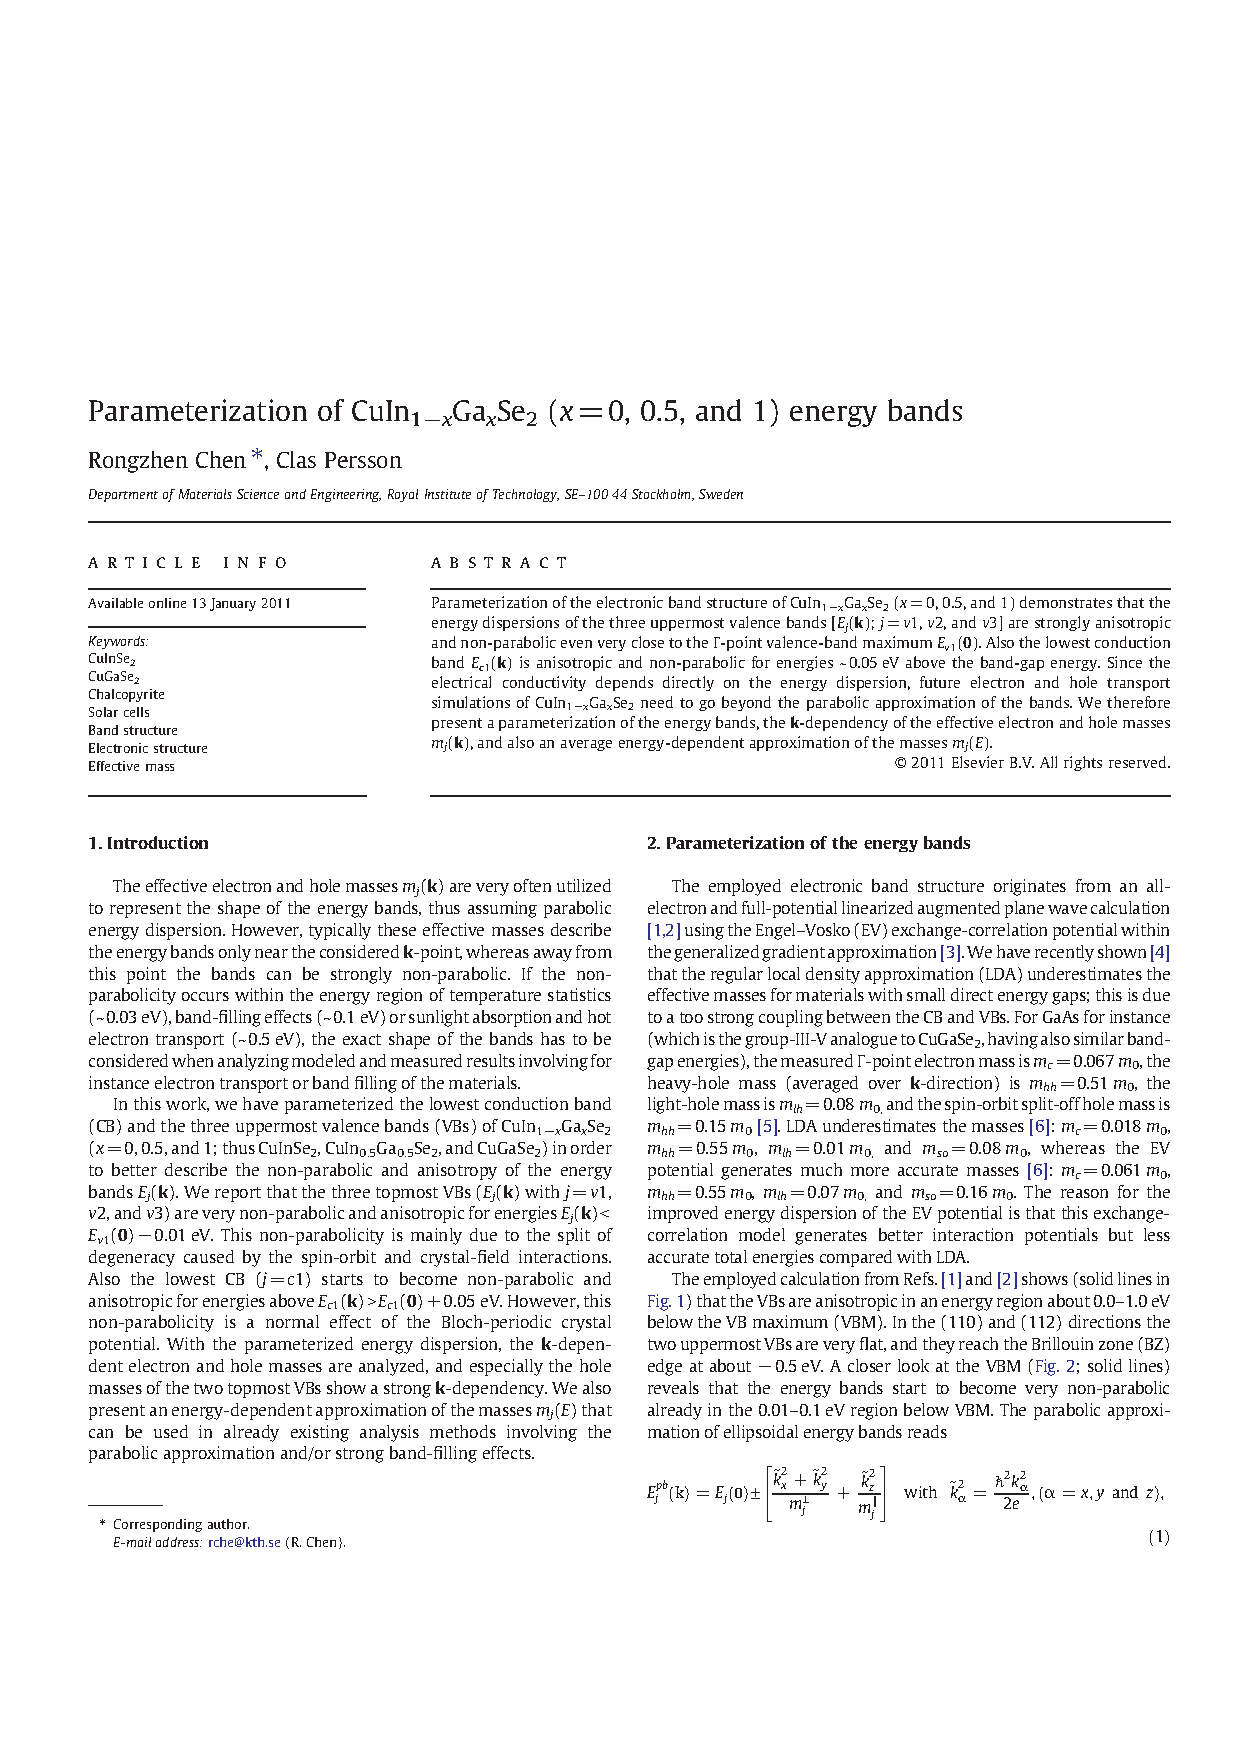
\includepdf[pages=-,templatesize={145mm}{200mm},noautoscale=true,offset=-97 40, pagecommand={}]{paper1new11.pdf}
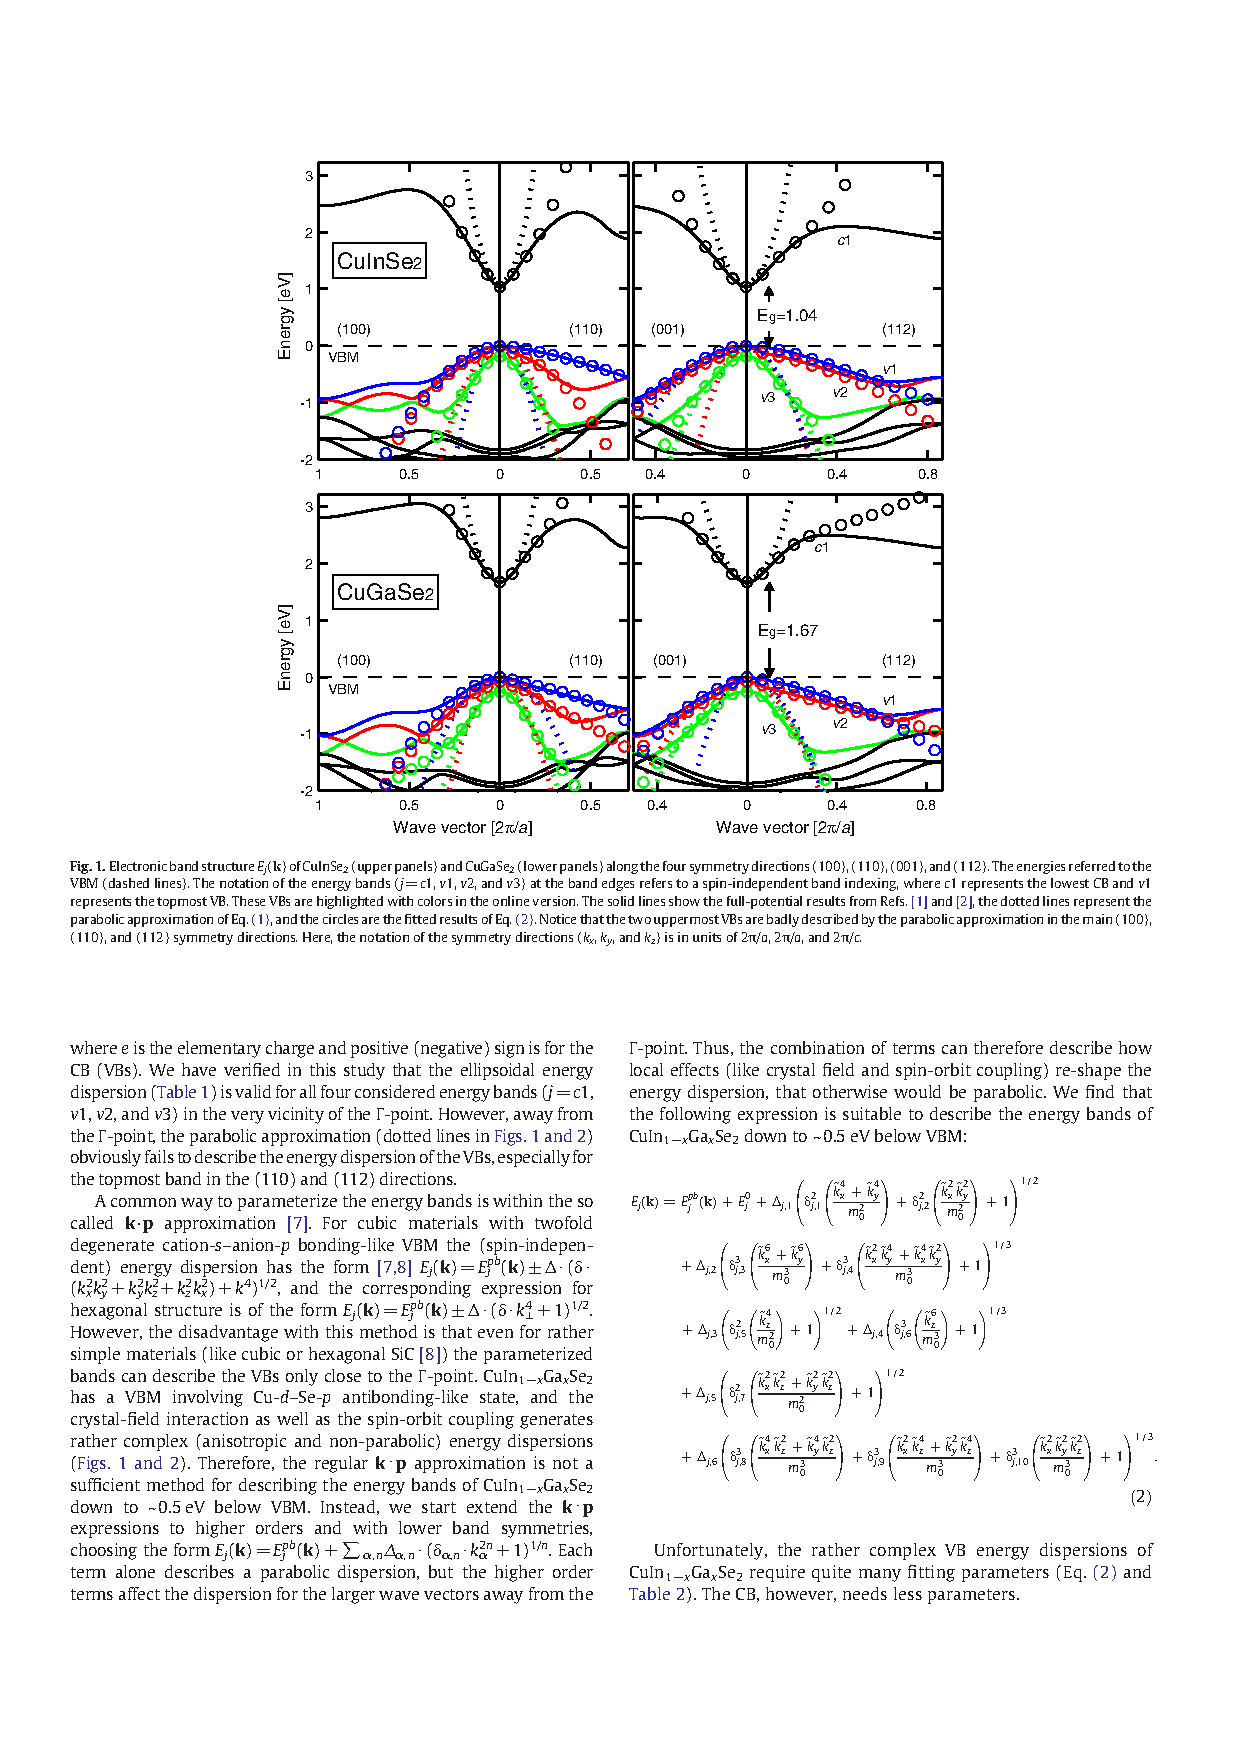
\includepdf[pages=-,templatesize={145mm}{200mm},noautoscale=true,offset=-97 -100, pagecommand={}]{paper1new111.pdf}


\section{Paper II: "Band-edge density-of-states and carrier concentrations in intrinsic and $p$-type CuIn\textsubscript{1-x}Ga\textsubscript{x}Se\textsubscript{2}"}
\textbf{R. Chen} and C. Persson, \textit{J. Appl. Phys.} {\textbf {112}}, 103708 (2012).



\newpage
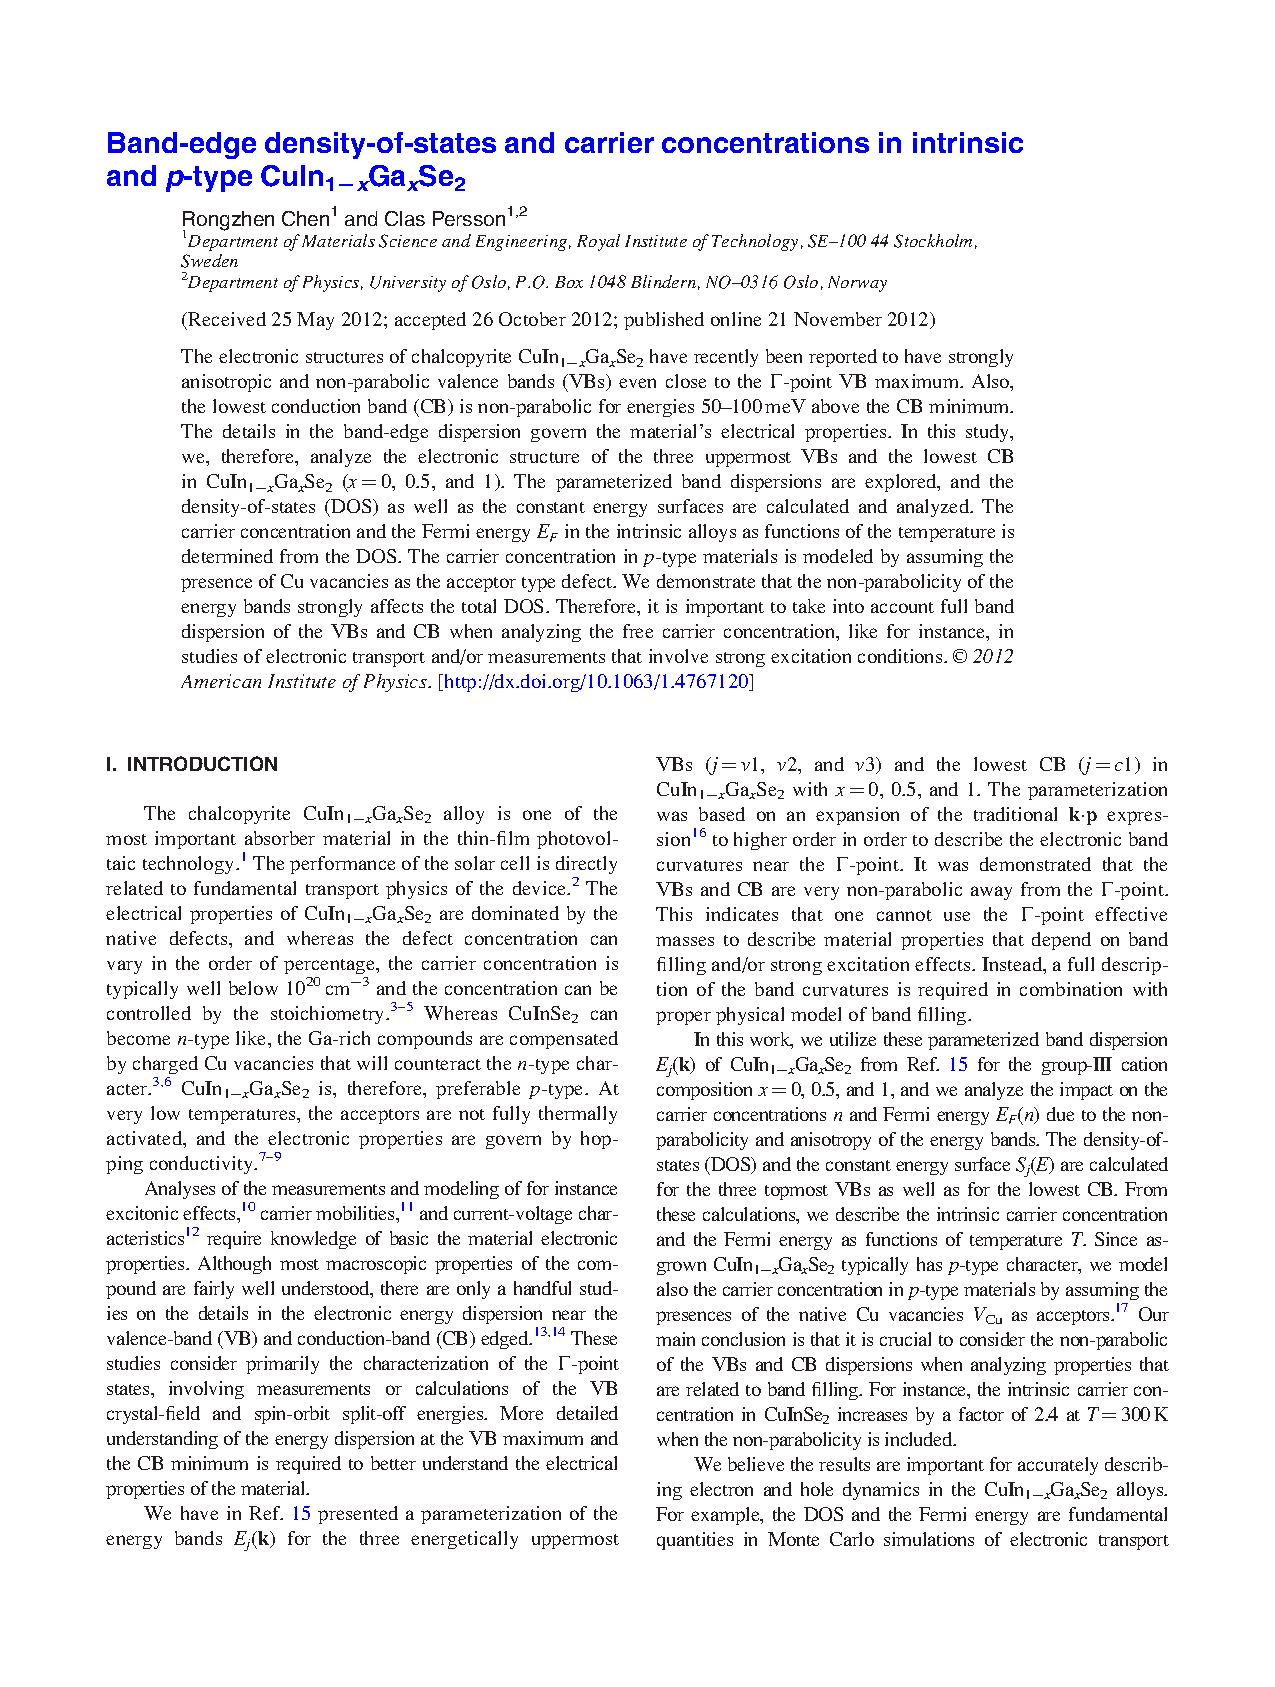
\includepdf[pages=-,templatesize={145mm}{200mm},noautoscale=true,offset=-97 -100, pagecommand={}]{paper2new11.pdf}
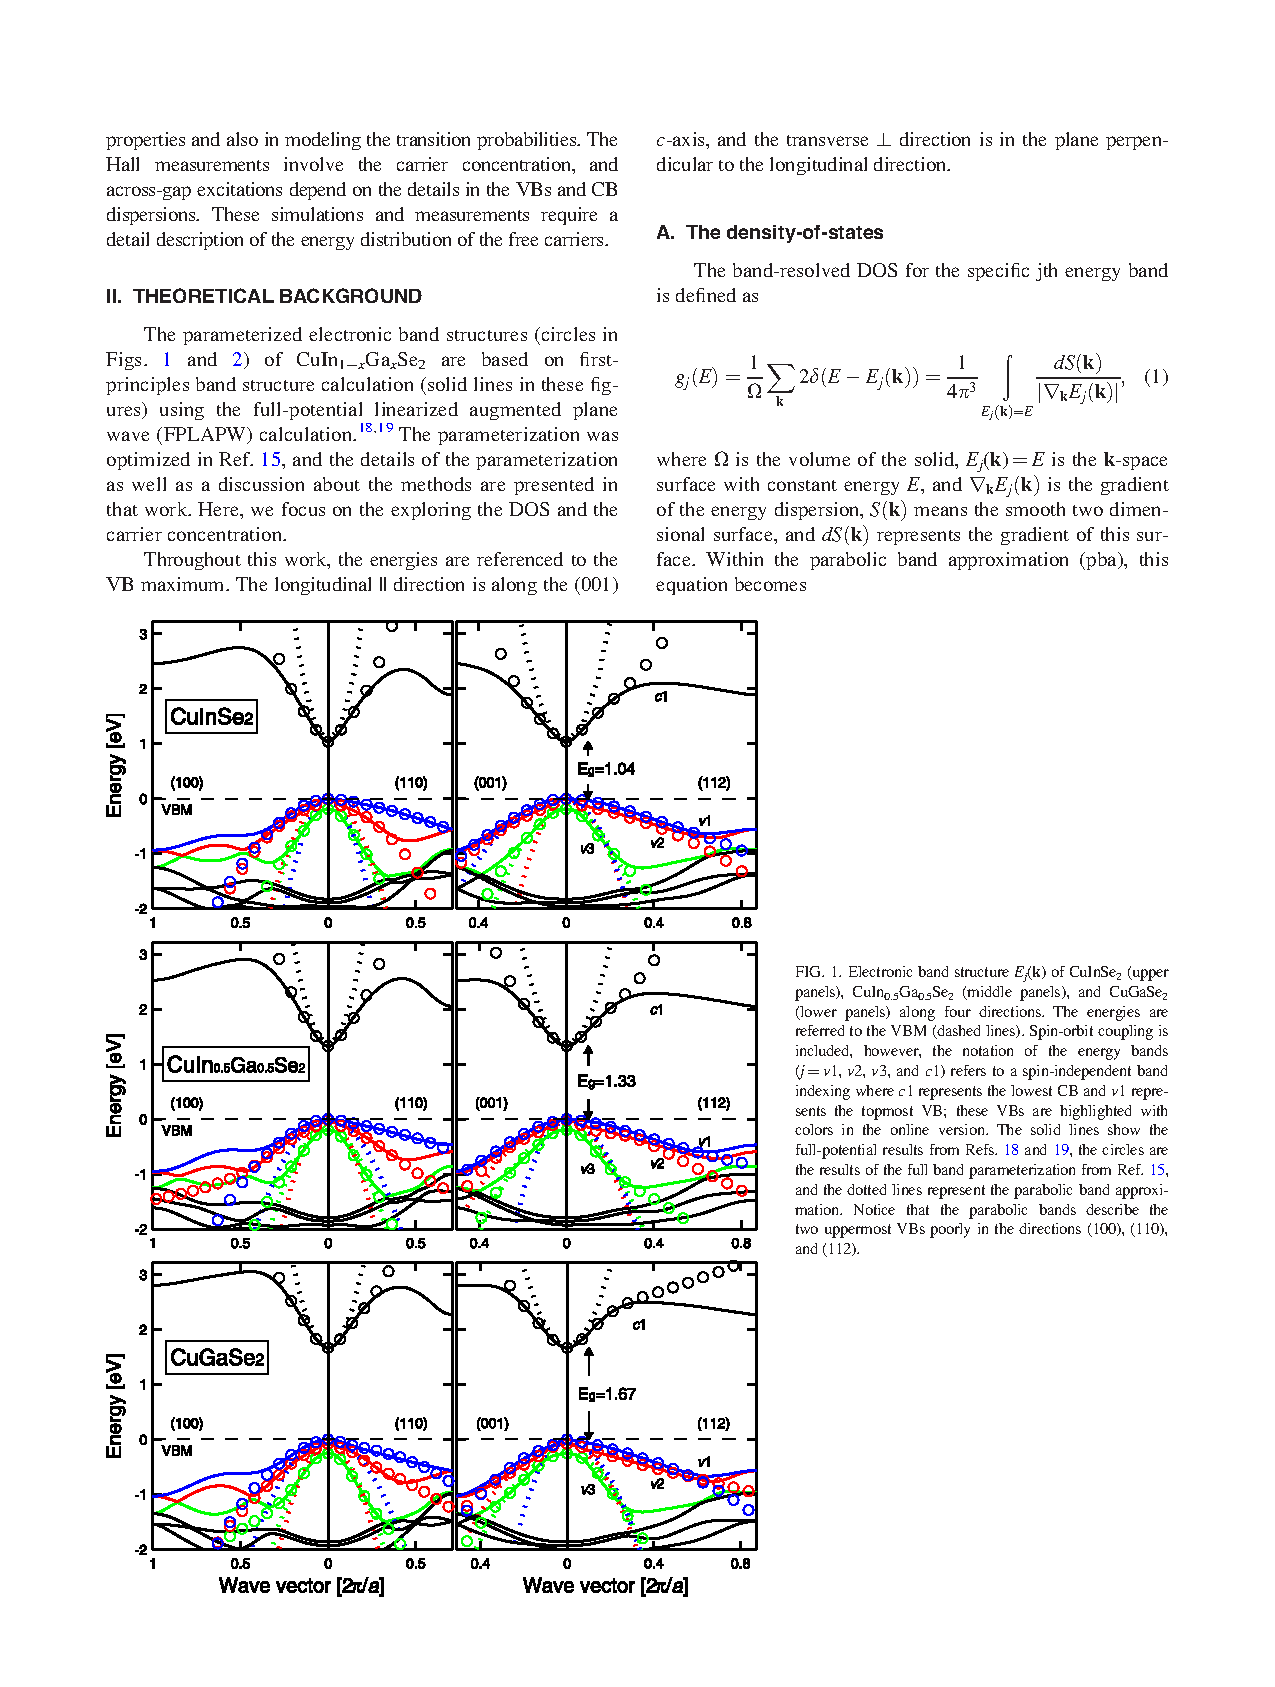
\includepdf[pages=-,templatesize={145mm}{200mm},noautoscale=true,offset=-97 -150, pagecommand={}]{paper2new111.pdf}

\section{Paper III: "Dielectric function spectra at 40 K and critical-point energies for CuIn\textsubscript{0.7}Ga\textsubscript{0.3}Se\textsubscript{2}"}
S.G. Choi, \textbf{R. Chen}, C. Persson, T.J. Kim, S.Y. Hwang, Y. D. Kim, and L. M. Mansfield,
\textit{Appl. Phys. Lett. } {\textbf {101}}, 261903 (2012).



\newpage
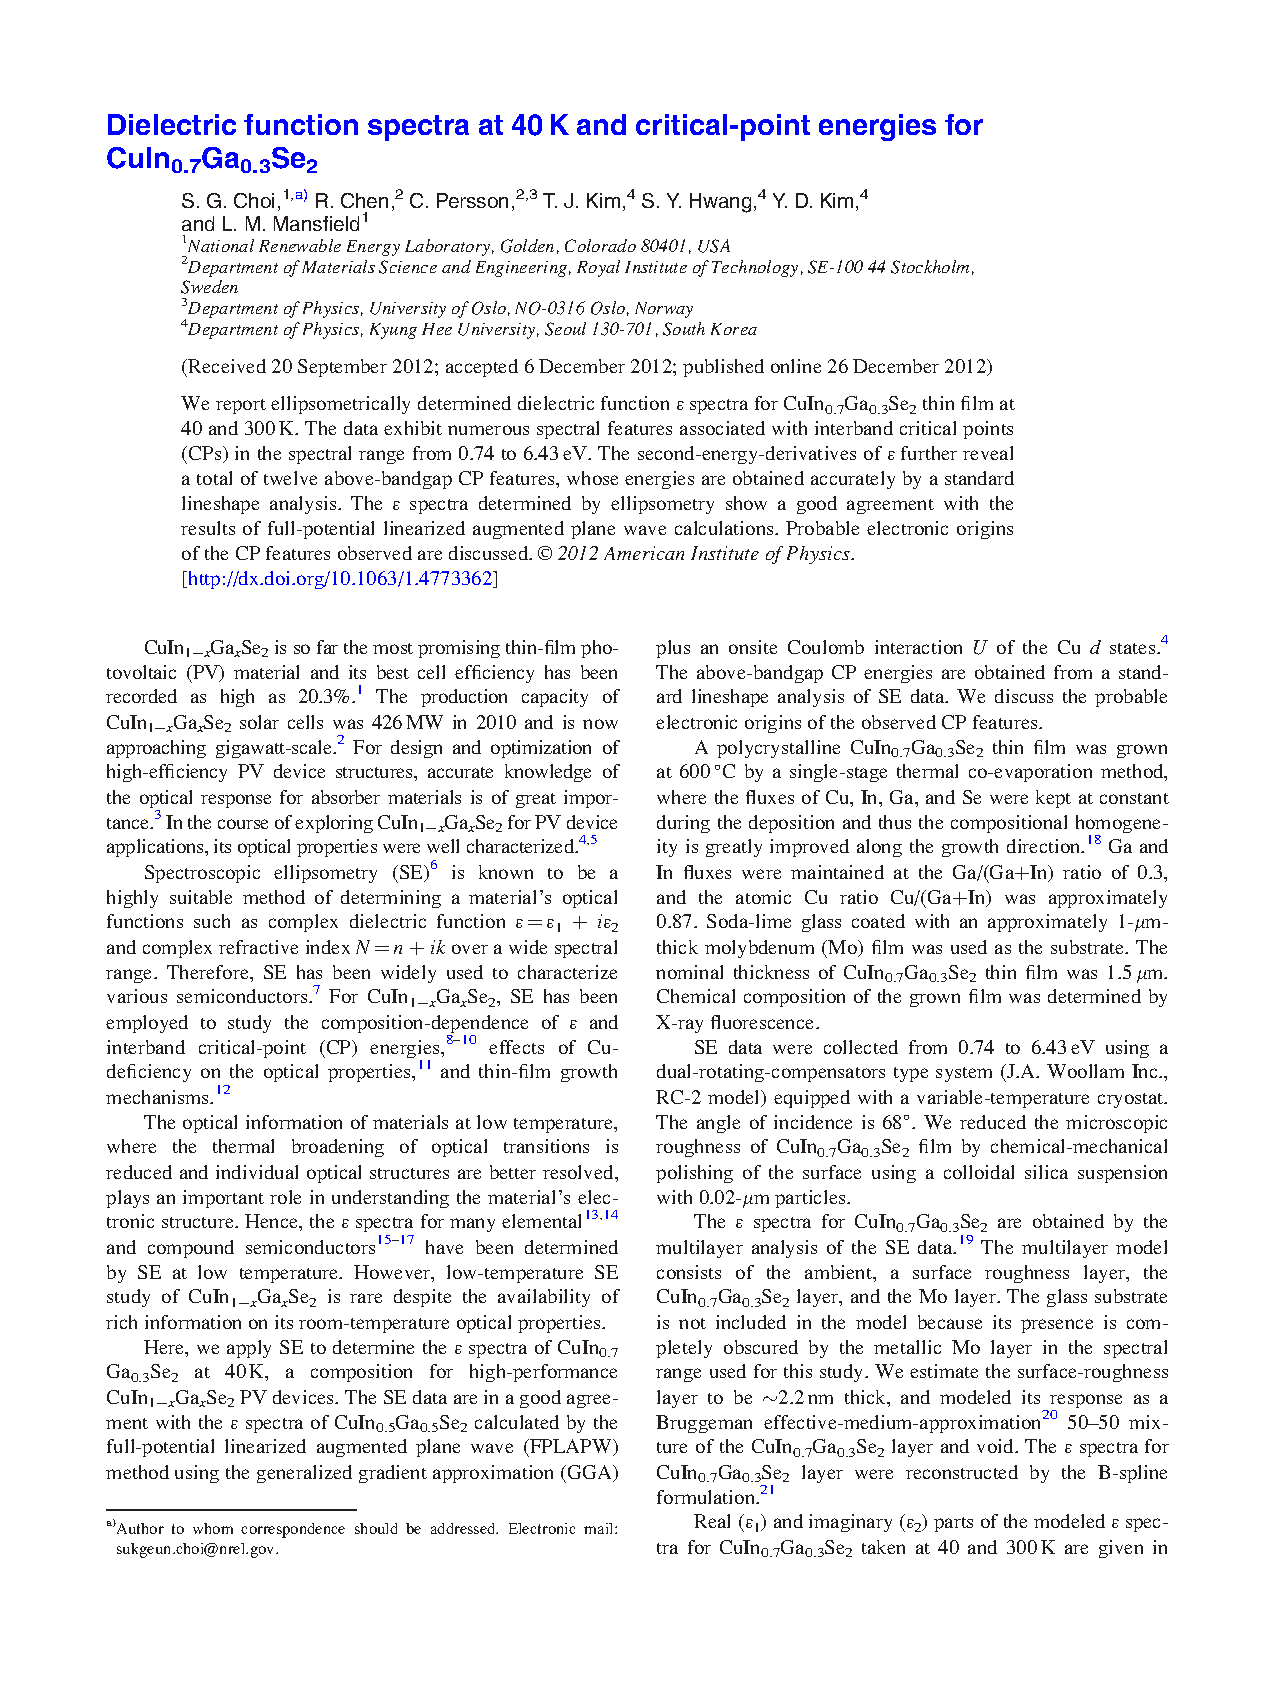
\includepdf[pages=-,templatesize={145mm}{200mm},noautoscale=true,offset=-97 -100, pagecommand={}]{paper3new11.pdf}
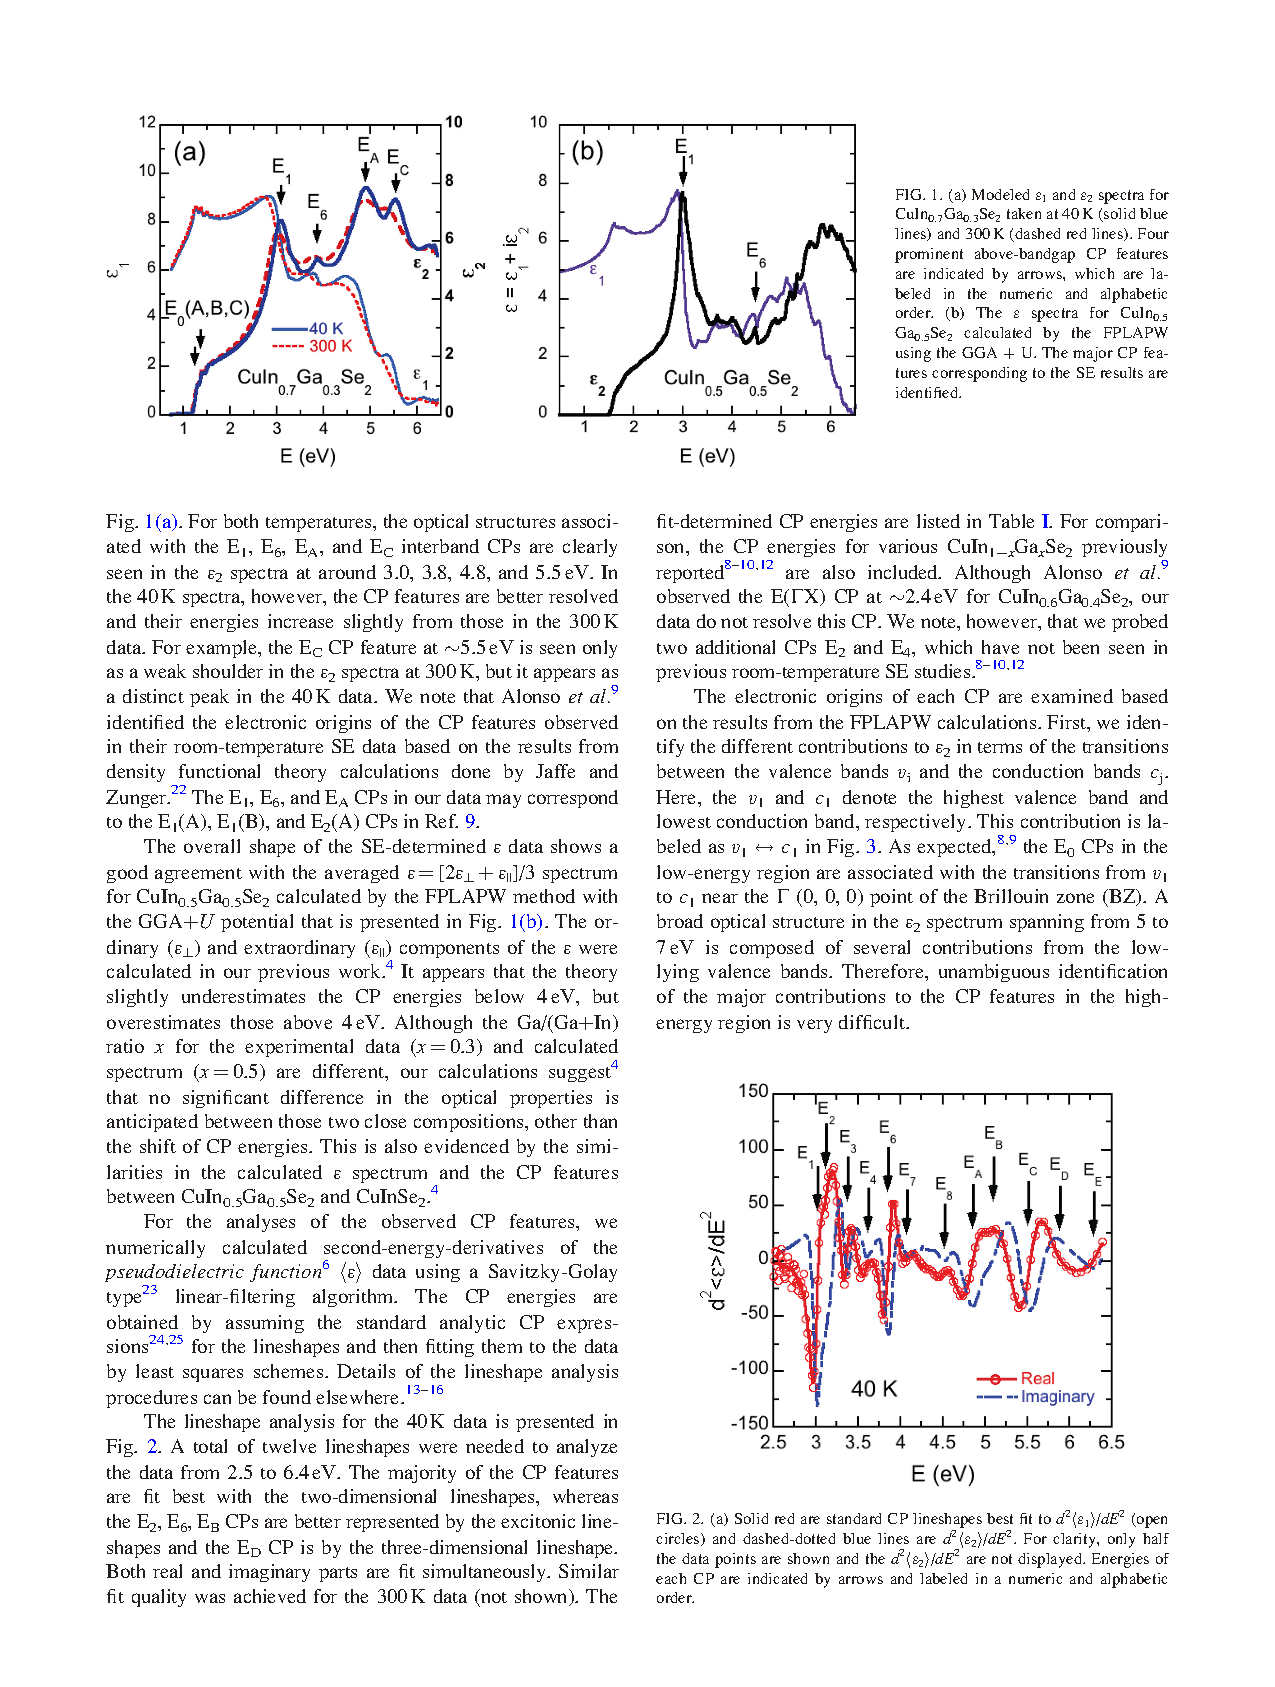
\includepdf[pages=-,templatesize={145mm}{200mm},noautoscale=true,offset=-97 -150, pagecommand={}]{paper3new111.pdf}

\end{document}
